\documentclass[openany]{book}

\usepackage[total={18cm,21cm}, top=2cm, left = 2cm]{geometry}
\parindent=0mm
\usepackage[T1]{fontenc}
\usepackage[utf8]{inputenc}
\usepackage[spanish, es-tabla]{babel}
\usepackage{xcolor}
\usepackage{pstricks}
\usepackage{graphicx}
\usepackage{tikz, tkz-tab}
\usepackage{setspace}
\usepackage{amsthm}
\usepackage{amsmath}
\usepackage{amssymb}
\usepackage{amsfonts}
\usepackage{tcolorbox}
\usepackage{textcomp}
\usepackage{courier}
\usepackage{tocloft}
\usepackage{titlesec}
\usepackage{multirow}
\usepackage{multicol}
\usepackage{longtable}


\definecolor{consoleback}{RGB}{245, 245, 245}
\definecolor{consoleprompterback}{RGB}{225, 225, 225}

\newcommand{\fx}{$f(x)$}
\newcommand{\arrowprompter}{\tcbox[colback=consoleprompterback,left=0pt,right=0pt,top=5pt,bottom=2pt,boxsep=0pt,arc=0pt,boxrule=0pt, on line]{{\black \texttt{>}}}}
\newcommand{\spaceprompter}{\tcbox[colback=consoleprompterback,left=0pt,right=0pt,top=10pt,bottom=2pt,boxsep=0pt,arc=0pt,boxrule=0pt, on line]{{\black \texttt{~}}}}

\newcommand{\arrowcode}[1]{\arrowprompter\texttt{#1}}
\newcommand{\spacecode}[1]{\spaceprompter\texttt{#1}}
\newcommand{\outcode}[1]{\texttt{#1}}
\newcommand{\linecode}[1]{\texttt{#1}}
\newcommand{\codecomment}[1]{{\it {\gray $\leftarrow$ #1}}}
\newcommand{\layoutcomment}[2]{{\it {\gray\texttt{#1}$\downarrow$ #2}}}
\newcommand{\linetab}{\texttt{\gray ~~~~}}

\newtcolorbox{fxcode}{colback=consoleback, arc=0pt, boxrule=0pt,boxsep=0pt,left=0pt,top=0pt,right=0pt,bottom=0pt}

\newtheorem{example}{Ejemplo}
\renewcommand{\theexample}{\arabic{chapter}.\arabic{section}.\arabic{example}}

\newtheorem{observation}{Observación}
\renewcommand{\theobservation}{\arabic{chapter}.\arabic{section}.\arabic{observation}}

\newcommand{\citar}[1]{{\red (citar: #1)}}
\newcommand{\backslashchar}{\char`\\}

\newcommand{\R}{\mathbb{R}}
\newcommand{\N}{\mathbb{N}}
\newcommand{\Z}{\mathbb{Z}}

\begin{document}
   \title{\Huge \fx\\Manual de Function 0.5}
   \author{Ivar Wiligran Vilca Quispe}
   \date{Diciembre de 2019}
   \maketitle
   
   \addtocontents{toc}{\hfill \textbf{Pág.} \par}
   \tableofcontents
   \decimalpoint{.}
   
   \titleformat{\chapter}[hang]{\Large\bfseries}{\thechapter.}{10pt}{\bf}
   \titlespacing{\chapter}{0pt}{10pt}{20pt}
   
   \titleformat{\section}[hang]{\large\bfseries}{\thesection.}{10pt}{\bfseries}
   \titlespacing{\section}{0pt}{10pt}{10pt}
%--------------------
   \addcontentsline{toc}{chapter}{Introducción}
\chapter*{Introducción}

   
\chapter{Primeros pasos con Function v0.5}
   En este capitulo se echa un vistazo rápido a las características y usos del software Function v0.5.
   
   \section{¿Qué es Function v0.5?}
      Function v0.5 es un software para evaluación de expresiones matemáticas, programación de funciones y algoritmos de manera sencilla y elegante con un lenguaje construido sobre una variante extendida de las expresiones lambda.% ademas Function v0.5 es software---.
      
   \section{Descarga e instalación}
   
   \section{La interfaz}
      Al ejecutar Function v0.5 se despliega la consola de comandos (o {\it shell} en ingles), en esta aparece un puntero representado por ``\arrowprompter'' desde el cual podemos ingresar el código a ser interpretado una vez que presionemos la tecla {\it RETURN}, tales códigos pueden ser evaluar una expresion, construir una nueva función, controlar el sistema, etc. 
   
      \begin{figure}[htbp]
         \caption{Interfaz gráfica}\label{fg:console}
         \begin{center}
            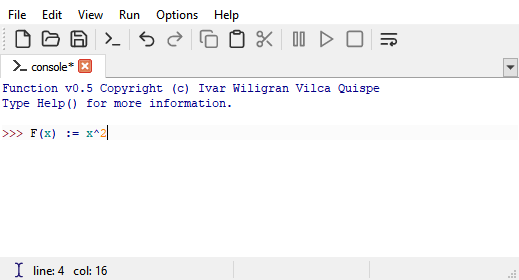
\includegraphics[scale=2.5]{FunctionImg1.png}
         \end{center}   
      \end{figure}
      
      Por ejemplo escribamos \texttt{35 + 12\^{}(1/2) - 4*Sin(-1.45)} después del puntero y ahora presionemos la tecla {\it RETURN}:
      
      \begin{fxcode}
         \arrowcode{35 + 12\^{}(1/2) - 4*Sin(-1.45)}\\
         \outcode{42.4349535792881} \codecomment{el resultado de sumar $2 + 3$}
      \end{fxcode}
      
      Esta es el resultado de evaluar la expresion $35 + 12^{1/2} - 4*\sin(-1.45)$
   
   \section{El lenguaje}
      Function v0.5 interpreta comandos que es un código que representa un bloque básico de ejecución, en total son 8 clases de comandos:
      
      \begin{longtable}[c]{ll}
         \caption{Lista de comandos}\label{tb:cmds} \\ \hline
         {\bf Nombre}      & {\bf Ejemplo} \\ \hline
         Ejecutar guiones  & \texttt{run "lib\textbackslash\textbackslash prelude.fx"} \\
         Notaciones        & \texttt{infixl 175 +} \\
         Sinónimo de tipo  & \texttt{String ::= [char]} \\
         Tipado heredable  & \texttt{f :: real -> real} \\
         Definiciones      & \texttt{f(x) := x\^{}2 + 2*x - 1} \\
         Asignaciones      & \texttt{x <- [[1, 0], [0, 1]]} \\
         Limpieza          & \texttt{clear f} \\
         Evaluación        & \texttt{2 + 3*x} \\
      \end{longtable}
      
      Ejecutar un guion significa interpretar todos los comandos escritos en un archivo de texto que contiene código Function v0.5 este archivo es llamado guion (o {\it script} en ingles).
      
      \begin{fxcode}
         \arrowcode{run "lib\textbackslash\textbackslash acme\textbackslash\textbackslash emptyscript.fx"}
      \end{fxcode}
      
      Los guiones suelen tener por defecto la extensión ``.fx''.
      
      Una definición se puede hacer directamente escribiendo una función con su respectiva expresion de retorno.
      
      \begin{fxcode}
         \arrowcode{f(x) := x\^{}3 + x - 3}
      \end{fxcode}
      
      Las asignaciones evalúan una expresión y la asignan a una variable o identificador pero sin mostrar el resultado.
      
      \begin{fxcode}
         \arrowcode{v <- 12*2 - 1}
      \end{fxcode}
      
      Para saber el valor de la variable se puede proceder a evaluarla:
      
      \begin{fxcode}
         \arrowcode{v}\\
         \outcode{23}
      \end{fxcode}
      
      La evaluación de expresiones es un comando que evalúa una expresión y luego muestra su resultado.
      
      \begin{fxcode}
         \arrowcode{23 + 4*5 - 2*(7 + 1)/(3\^{}4) + (-4)}\\
         \outcode{38.8024691358025}
      \end{fxcode}
      
      Para conocer nuevamente el valor de la evaluación anterior se puede utilizar la función \texttt{Ans()}.
      
      \begin{fxcode}
         \arrowcode{Ans()}\\
         \outcode{38.8024691358025}
      \end{fxcode}
      
      El valor de esta función cambia cada vez que se ejecute un comando de evaluación.
      
      Algunas de las funciones y operadores en Function v0.5 son:
      
      \begin{longtable}[c]{|l|c|l|l|l|}
         \caption{Funciones y operadores básicos}\label{tb:basicopr} \\ \hline
         {\bf Nombre}           & {\bf Símbolo} & {\bf Ejemplo} & {\bf Resultado}  & {\bf Descripción}\\ \hline
         suma           & \texttt{+} & \texttt{3 + 4} & \texttt{7}  & suma de números reales\\ \hline
         resta          & \texttt{-} & \texttt{4 - 1} & \texttt{3}  & resta de números reales\\ \hline
         multiplicación & \texttt{*} & \texttt{5 * 5} & \texttt{25}  & multiplicación de números reales\\ \hline
         división       & \texttt{/} & \texttt{4 / 16} & \texttt{0.25}  & División de números reales\\ \hline
         potenciación   & \texttt{\^} & \texttt{4~\^~0.5} & \texttt{2}  & Potenciación de números reales\\ \hline
         negación   & \texttt{-} & \texttt{- 3.56} & \texttt{-3.56}  & el negativo de un número\\ \hline
         seno & \texttt{Sin} & \texttt{Sin(0.7512)} & \texttt{0.6825162} & La función seno \\ \hline
         coseno & \texttt{Cos} & \texttt{Cos(0.7512)} & \texttt{0.730870} & La función coseno \\ \hline
         tangente & \texttt{Tan} & \texttt{Tan(0.7512)} & \texttt{0.933840} & La función tangente \\ \hline
         arco seno & \texttt{ASin} & \texttt{ASin(0.7512)} & \texttt{0.8498781} & La función arco seno \\ \hline
         arco coseno & \texttt{ACos} & \texttt{ACos(0.7512)} & \texttt{0.7209181} & La función arco coseno \\ \hline
         arco tangente & \texttt{ATan} & \texttt{ATan(0.7512)} & \texttt{0.6442686} & La función arco tangente \\ \hline
      \end{longtable}
      
      Se pueden utilizar los tabuladores para crear espacios mas rápidamente, estos tabuladores tienen un tamaño equivalente a 8 espacios en blanco.
      
   \section{Control del sistema}
      Para realizar algunas órdenes para el sistema como por ejemplo cerrar el software se pueden recurrir a las funciones siguientes que ademas de devolver un valor realiza una acción.
      
      \begin{longtable}[c]{|l|l|l|}
         \caption{Ordenes básicas}\label{tb:basicord} \\ \hline
         {\bf Nombre} & {\bf Representación} & {\bf Descripción}\\ \hline
         respuesta    & \texttt{Ans()} & devuelve el resultado de la expresion anterior evaluada\\ \hline
         ayuda    & \texttt{Help()} & despliega la ayuda básica de Function v0.5\\ \hline
         reiniciar & \texttt{Restart()} & reinicia el sistema\\ \hline
         interrumpir    & \texttt{Interrupt()} & interrumpe una tarea llevada a cabo por Function v0.5\\ \hline
         salir    & \texttt{Quit()} & finaliza el sistema y cierra el programa\\ \hline
      \end{longtable}
      
      \begin{fxcode}
         \arrowcode{Ans()}\codecomment{resultado}
      \end{fxcode}
      
      \begin{fxcode}
         \arrowcode{Help()}\codecomment{ayuda}
      \end{fxcode}
      
      \begin{fxcode}
         \arrowcode{Restart()}\codecomment{reiniciar}
      \end{fxcode}
      
      \begin{fxcode}
         \arrowcode{Interrupt()}\codecomment{interrumpir}
      \end{fxcode}
      
      \begin{fxcode}
         \arrowcode{Quit()}\codecomment{salir}
      \end{fxcode}
      
      Similar a la función del sistema \texttt{Interrupt()} existe un atajo para cuando la ejecución de un comando se hace demasiado largo se pueda abortar su ejecución, esto se consigue presionando la combinación de teclas {\it Ctrl+BREAK} que interrumpe la ejecución y vuelve a mostrar el puntero.
      \\
      
      Por ultimo si se ingresa un carácter no reconocido o le falta algún argumento a los operadores, el sistema Function v0.5 detecta dicho error y lanza un mensaje indicando nuestro error.
      
      \begin{fxcode}
         \arrowcode{¿}\\
         \outcode{ERROR - lexical error in command 1 line 1, unexpected input "¿"}
      \end{fxcode}
      
      \begin{fxcode}
         \arrowcode{2 + }\\
         \outcode{ERROR - syntax error in command 1 line 1, missing right argument for "\texttt{+}"}
      \end{fxcode}
      
   
   
   
   
   
   
   
   
   
   
   
   
   \chapter{Comandos}
   Los comandos son los bloques básicos de ejecución formados por código Function v0.5 mediante el cual el sistema sabe que hacer y como actuar.
   
   \section{Tokens}
      Las unidades léxicas con los que se trabaja se le llaman tokens, ejemplos de tokens pueden ser números, identificadores, símbolos, cada uno de los lados de un paréntesis, etc.
      
      Por ejemplo en el siguiente código(que representa una expresion) \texttt{35 + 12\^{}(1/2) - 4*Sin(-1.45)} los tokens son:
      
      \texttt{35}, \texttt{+}, \texttt{12}, \texttt{\^{}}, \texttt{(}, \texttt{1}, \texttt{/}, \texttt{2}, \texttt{)}, \texttt{-}, \texttt{4}, \texttt{*}, \texttt{Sin}, \texttt{(}, \texttt{-}, \texttt{1.45} y \texttt{)}
      
   \section{Clases de comandos}
      Existen 8 clases de comandos los cuales son:
      
      \begin{longtable}[c]{lll}
         \caption{Comandos}\label{tb:commands} \\ \hline
         {\bf Nombre} & {\bf Ejemplo} & {\bf Descripción} \\ \hline &&\\
         Ejecutar & \texttt{run "lib\textbackslash\textbackslash prelude.fx"} &
         \begin{minipage}{7cm}
            Este comando sirve para interpretar el código Function v0.5 que se encuentra en un archivo de texto también llamado guion o script que por defecto tienen extensión ``.fx''.
         \end{minipage} \\ &&\\
         Notación & \texttt{infixl 175 +} &
         \begin{minipage}{7cm}
            Este comando sirve para definir la posición, prioridad y precedencia de un operador.
         \end{minipage}\\ &&\\
         Sinónimo de tipo & \texttt{String ::= [char]} &
         \begin{minipage}{7cm}
            Este comando sirve para darle un nombre a un tipo de dato y simplificar el posteriores usos.
         \end{minipage}\\ &&\\
         Tipado heredable & \texttt{f :: real -> real} &
         \begin{minipage}{7cm}
            Sirve para establecer el tipo de dato que tendrá las posteriores definiciones de una función o constante.
         \end{minipage}\\ &&\\
         Definición & \texttt{f(x) := x\^{}3 - x\^{}2 + 1} &
         \begin{minipage}{7cm}
            Sirve para definir nuevas funciones o constantes.
         \end{minipage}\\ &&\\
         Asignación & \texttt{x <- 23*12 + 1} &
         \begin{minipage}{7cm}
            Sirve para otorgarle un valor a una variable o identificador para posteriores usos.
         \end{minipage}\\ &&\\
         Limpieza & clear f &
         \begin{minipage}{7cm}
            Este comando elimina cualquier definición, valor, etc. asociado a un identificador.
         \end{minipage}\\ &&\\
         Evaluación & \texttt{12*12\^{}2 - 3*(4 + 5)} &
         \begin{minipage}{7cm}
            Este comando evalúa la expresion e imprime el resultado.
         \end{minipage}\\
      \end{longtable}
      
      Como se ve todos los comandos pueden ser ingresados tanto desde la consola como en archivos guiones. Para interpretar un comando desde la consola se debe presionar la tecla {\it RETURN}.
      
   \section{Comandos multilínea y la regla del sangrado}
      Los comandos pueden ser escritos en una sola linea o en varias, desde un guion esto no supone un problema pues los editores de texto son de múltiples lineas, pero desde la consola para ingresar mas lineas se debe colocar los puntos suspensivos ``\texttt{...}'' al final de una linea y luego presionar {\it RETURN} y cuando ya se han terminado de escribir todas las lineas nuevamente presionar {\it RETURN} esta vez sin puntos suspensivos para que sean interpretados.
   
      Al ingresar mas lineas desde la consola Function v0.5 no restringe la cantidad de comandos que se puedan ingresar por lo que pueden ser mas de uno pero que se interpretan de uno en uno y en orden.
      
      \begin{fxcode}
         \arrowcode{10 + 3 * 3 ...}\\
         \spacecode{~~~\texttt{-} (12 + ...}\\
         \spacecode{~~~4) ...}\\
         \spacecode{-2 + 7}\\
         \outcode{3}\\
         \outcode{5}
      \end{fxcode}
      
      Ahora bien, ¿Como sabe Function v0.5 que en el anterior código hay exactamente dos comandos? pues, Function v0.5 tiene lo que se conoce como sintaxis bidimensional llamado sangrado (o {\it layout} en ingles) lo cual se puede resumir como:
      
      \begin{enumerate}
         \item Para un nuevo comando, el primer carácter de su primer token establece o marca la columna de sangrado del comando de manera que para los demás tokens sean considerados como parte del comando estas deben empezar en una columna mayor a la columna marcada y en la misma o posteriores lineas.
         \item Si un token inicia en la misma o antes de la columna de sangrado entonces establece el inicio de un nuevo comando con su propio sangrado.
      \end{enumerate}
      
      \begin{fxcode}
         \layoutcomment{~}{aquí marca la columna de sangrado}\\
         \arrowcode{g(y) := y\^{}4 + ...}\\
         \spacecode{ y} \codecomment{si pertenece al comando pues su columna es mayor que la columna de sangrado}
      \end{fxcode}
      \begin{fxcode}
         \arrowcode{12 * 3 ...}\\
         \spacecode{- 2} \codecomment{ya no es parte del anterior comando pues ``\texttt{-}'' empieza en la misma columna de sangrado}
      \end{fxcode}
      \begin{fxcode}
         \arrowcode{~~v <- 12 ...}\\
         \spacecode{- 1} \codecomment{tampoco es parte del anterior comando pues ``\texttt{-}'' empieza muy atrás de la columna de sangrado}
      \end{fxcode}
   
      Para realizar un sangrado rápido se puede utilizar el tabulador que por defecto tiene el tamaño equivalente a 8 espacios en blanco.
      
      \begin{fxcode}
         \arrowcode{y <- 23 * 14 ...}\\
         \spacecode{~~~~~~~\texttt{-} 15 + 5\^{}(1/2)}
      \end{fxcode}
   \section{Comentarios}
      Los comentarios son ciertas partes del código en el que se describe o se comenta algo sobre las expresiones o acerca del código pero que son ignorados por el interprete, en Function v0.5 los comentarios son secuencias de caracteres que tienen la forma:
         
         \texttt{...<texto en una sola linea>}
      
      donde \texttt{<texto en una sola linea>} es cualquier texto que termina al final de la linea, los comentarios pueden ir tanto en la consola como en los guiones.
      
      \begin{fxcode}
         \arrowcode{...este es un comentario}
      \end{fxcode}
      \begin{fxcode}
         \arrowcode{2 + 3 ...este texto será ignorado}
      \end{fxcode}
      
      Los puntos suspensivos marcan el inicio del comentario pero si inmediatamente antes de los puntos suspensivos se encuentra un carácter simbólico ya no se interpretara como el inicio de un comentario sino como un identificador simbólico.
      
      \begin{fxcode}
         \arrowcode{*... 0}
      \end{fxcode}
      
      En el código anterior los puntos suspensivos esta inmediatamente precedidos por ``\texttt{*}'' por lo que el sistema lo interpreta como el token ``\texttt{*...}'' y ya no forma un comentario.
      
   \section{Consola multilínea}
      Como se vio mas antes los puntos suspensivos son utilizados para poder ingresar mas lineas de código desde la consola pues por defecto al presionar {\it RETURN} ingresa una sola linea, lo que realmente sucede es que si hay un comentario al final de una linea en la consola Function v0.5 permitirá que el usuario ingrese una nueva linea antes de interpretar el código y esta vez de varias lineas.
      
      \begin{fxcode}
         \arrowcode{2 + 3 ...esto es un comentario}\\
         \spacecode{~* 4}\\
         \outcode{14}\\
         \arrowcode{1 ...}\\
         \spacecode{~\texttt{-} 3}\\
         \outcode{-2}
      \end{fxcode}
   
      Este comportamiento de los comentarios solo es valido y útil en la consola, cuando se editan códigos Function v0.5 en archivos separados (llamados guiones) no es necesario pues los editores son multilinea y los comentarios son utilizados solo para su propósito original: comentar el código.
      
      \begin{fxcode}
         \linecode{...Este es un archivo de texto con código Function v0.5 o "guion"}\\
         \linecode{v <- 1}\\
         \linecode{f(x) := x\^{}2 + 2*x - v}\\
         \linecode{f(3) * }\\
         \linecode{~~~~12} \codecomment{he aquí un comando multilinea y no necesita puntos suspensivos}
      \end{fxcode}
   
   
   
   
   
   
   
   
   
   
   
   
   
   
   
   
   
   
   
   
   
\chapter{Evaluación de expresiones}
   Las expresiones son combinaciones de funciones, operadores, números, valores y otras formas.

   En este capítulo se explicará algunas clases de expresiones útiles como los átomos y las aplicaciones ya en los siguientes capítulos se presentaran mas formas de expresiones y ademas sobre el comando de evaluación de expresiones.

   \section{Evaluación}
      La evaluación de expresiones es una parte fundamental de Function v0.5, para hacer la evaluación simplemente se escribe una expresion después del puntero en la consola y se presiona {\it RETURN}.
      
      \begin{fxcode}
         \arrowcode{2*(4 + 2)\^{}2 - 12} \codecomment{la expresion esta formada con operadores}\\
         \outcode{60}\\
         \arrowcode{Sin(2*Exp(12)) + Cos(1)} \codecomment{la expresion esta formada con funciones}\\
         \outcode{0.794268198798373}
      \end{fxcode}
      
      Las expresiones deben estar correctamente formadas, por ejemplo en el siguiente código habrá un error al usar los paréntesis.
      
      \begin{fxcode}
         \arrowcode{4*233 + (23} \codecomment{no se a cerrado el paréntesis}
      \end{fxcode}
      
      A veces existen funciones que tiene varios parámetros como la función \texttt{ATan2} que toma dos argumentos \texttt{x} y \texttt{y} devolviendo el arco tangente de $y/x$.
      
      \begin{fxcode}
         \arrowcode{ATan2(1, 1) + Cos(1)}\\
         \outcode{1.32570046926559}
      \end{fxcode}
      
      En algunos casos no es necesario el uso de paréntesis para las funciones que tienen un solo argumento y se pueden obviar.
      
      \begin{fxcode}
         \arrowcode{Exp 2 + Ln(3 + 4)}\\
         \outcode{9.33496624798596}
      \end{fxcode}
      
      En este ejemplo vemos que para la exponencial no es necesario el uso de paréntesis pues su argumento es solo el numero 2 en cambio para el logaritmo su argumento esta basado en una expresion por lo que si es necesario agruparlo entre paréntesis.
      \\
      
      Para saber el resultado de una evaluación anterior se puede recurrir al uso de la función \texttt{Ans()}.
      
      \begin{fxcode}
         \arrowcode{Ans()}\\
         \outcode{9.33496624798596} \codecomment{resultado de $\exp(2) + \ln(3 + 4)$}
      \end{fxcode}
      
      El valor que devuelve la función \texttt{Ans()} cambia cada vez que se ejecuta el comando de evaluación.
      
      Los operadores son en realidad funciones al que se a dotado de una notación particular, por ejemplo el operador + de suma es una función que toma dos argumentos y devuelve la suma de esos dos números, en Function v0.5 existen tres tipos de operadores los infijos, posfijos y prefijos aunque este ultimo es equivalente a la notación de una función, ejemplos de operadores infijos son +, -, *, / y de operadores posfijos ! (el operador de factorial) y de prefijos prácticamente todas las funciones pues no hay distinción entre operador prefijo y función.
      
      \begin{fxcode}
         \arrowcode{Abs 1 + 3!} \codecomment{Abs es la funcion de valor absoluto y ! es el factorial} \\
         \outcode{7}
      \end{fxcode}
      
      Los operadores pueden convertirse en su forma prefija al encerrarsele entre paréntesis.
      
      \begin{fxcode}
         \arrowcode{(+)(Abs 1, (!)3)}\\
         \outcode{7}
      \end{fxcode}
      
      En el código anterior se puede notar con mas claridad que el operador + (y todos los operadores infijos) es una función con dos argumentos.
      \\
      
      Cuando un operador o función esta "trabajando" sobre su argumento se dice que esa función u operador esta siendo aplicada a su argumento una función u operador aplicado a un argumento se le llama aplicación.
      \\
      
      El comando de evaluación de expresiones al igual que otros comandos tiene la regla de sangrado marcado por el primer token con el cual se inicia el comando, es decir para que un token (que no sea el primero) sea considerado como parte de la expresion a evaluar su columna de inicio debe ser mayor que el de la columna del primer token, en otro caso formaran un nuevo comando.
      \\
      
      \begin{fxcode}
         \arrowcode{2*(4 + 2)\^{}2 ...} \codecomment{ingresando varias lineas} \\
         \spacecode{~\texttt{-} 12} \codecomment{estos tokens son parte de la expresion a evaluar}\\
         \outcode{60}\\
         \arrowcode{2*(4 + 2)\^{}2 ...} 
         \spacecode{- 12} \codecomment{estos tokens ya no son parte de la expresion anterior}\\
         \outcode{72}\\
         \outcode{-12}
      \end{fxcode}
      
      Function v0.5 realiza evaluación estricta es decir siempre evalúa los argumentos sean o no sean necesarios antes de devolver el retorno.
      
   \section{Átomos}
      Las expresiones atómicas son expresiones que están formados por una sola unidad léxica y pueden ser números, caracteres, cadenas, valores lógicos o {\it booleanos} (también conocidos como valores de verdad)\citar{valores de verdad} y una expresion especial que indica el fallo o fracaso durante una operación.
      
      \subsection{Numero decimal}
      Un numero en base decimal es una secuencia de caracteres numéricos con un punto como separador decimal, en Function v0.5 esta formado como una unidad léxica que empieza por uno o varios caracteres numerales y que puede seguirlo el punto como separador decimal y también con un indicador de desplazamiento del punto decimal\citar{numero decimal}.\\
      
      Un {\it numero natural} es representado por una secuencia de caracteres {\bf numerales} ``\texttt{0123456789}''.
      
      \begin{fxcode}
         \arrowcode{3849578} \codecomment{un numero natural en Function v0.5}
      \end{fxcode}
      
      Un {\it numero real} se representa como una secuencia de caracteres numerales separados por un único punto ``\texttt{.}''.
      
      \begin{fxcode}
         \arrowcode{435.12345} \codecomment{este es un numero real en Function v0.5}
      \end{fxcode}
      
      Los numero naturales también son números reales, de hecho el numero $3849578$ se puede representar como $3849578.0$ ambas representaciones son equivalentes.
      
      Para representar números con signo se le antepone a un numero el simbolo ``\texttt{-}'' para números negativos o el simbolo ``\texttt{+}'' para números positivos(aunque lo ultimo no es necesario).
      
      \begin{fxcode}
         \arrowcode{-3849578.324}
      \end{fxcode}
      
      Los números también pueden estar en notación científica o coma flotante (punto en nuestro caso) para lo cual simplemente se adjunta por la derecha el carácter ``\texttt{E}'' en mayúscula o minúscula seguido de un número entero con signo o sin signo\citar{coma flotante}.
      
      \begin{center}
         \fcolorbox{consoleback}{consoleback}{\texttt{~~}{\large fE$\pm$d}\texttt{~~}}
      \end{center}
      
      Donde ``f'' es un número real con signo o sin signo llamado {\it mantisa} y ``$\pm$d'' es un número entero con signo o sin signo llamado {\it exponente}.
      
      \begin{fxcode}
         \arrowcode{325.E-4}
      \end{fxcode}
      
      \begin{fxcode}
         \arrowcode{-341e3}
      \end{fxcode}
      
      \begin{fxcode}
         \arrowcode{3478.4357e+1}
      \end{fxcode}
      
      Cabe indicar que para que una un numero sea válido su secuencia de caracteres no debe estar separado por espacios en blanco o algún otro carácter que no corresponde.
      
      \subsection{Numero hexadecimal}
      Los números hexadecimales son aquellos que tienen base 16\citar{numero hexadecimal}, Function v0.5 también permite representar números enteros en base hexadecimal como una secuencia de caracteres numerales y caracteres ``\texttt{abcdef}'' en mayúscula o minúscula al cual se le antepone ``\texttt{0x}'' con ``\texttt{x}'' en mayúscula o minúscula.\\
      
      \begin{fxcode}
         \arrowcode{0x41FFeA10} \codecomment{el numero $1107290640$ representado en base hexadecimal}
      \end{fxcode}
      
      \begin{fxcode}
         \arrowcode{0X4450BbA1}
      \end{fxcode}
      
      De igual manera que en los números decimales en el formato hexadecimal también se puede poner signo anteponiendo el simbolo ``\texttt{-}'' o ``\texttt{+}''.\\
      
      \begin{fxcode}
         \arrowcode{-0x24FFEE12}
      \end{fxcode}
      
      También en los números hexadecimales para que esta sea valida su secuencia de caracteres no debe estar separado por espacios en blanco o por otro carácter que no corresponde.\\
      
      Este tipo de representación es útil especialmente para visualizar las secuencias de bits de un número entero o realizar las operaciones a nivel de bits ya que cada dígito hexadecimal representa un nible binario (secuencia de cuatro bits)\citar{nibble y bits en hexadecimal}.\\
      
      \subsection{Infinitos y NAN}
      Un numero infinito es aquel numero que es lo mas grande posible o aquel resultante de la división por cero de un numero distinto de cero\citar{Infinitos} y NAN que significa ``Not A Number'' en ingles y representa el resultado de una operación numérica fallida o indeterminada como cuando se divide 0 entre 0\citar{NAN}, es decir es un átomo numérico invalido, en Function v0.5 los infinitos se representan por la palabra clave ``\texttt{inf}'' y NAN se representa por la palabra clave ``\texttt{nan}''.
      
      \begin{fxcode}
         \arrowcode{inf}
      \end{fxcode}
      
      \begin{fxcode}
         \arrowcode{inf}
      \end{fxcode}
      
      \begin{fxcode}
         \arrowcode{nan}
      \end{fxcode}
      
      \begin{fxcode}
         \arrowcode{1/0}\\
         \outcode{inf}
      \end{fxcode}
      
      \begin{fxcode}
         \arrowcode{0/0}\\
         \outcode{nan}
      \end{fxcode}
      
      Para generar los negativos de los infinitos o incluso de NAN (aunque para este ultimo no es necesario) se adjunta el simbolo ``\texttt{-}'' como a cualquier otro numero.
      
      \begin{fxcode}
         \arrowcode{-inf}
      \end{fxcode}
      
      \begin{fxcode}
         \arrowcode{-nan}\\
         \outcode{nan}
      \end{fxcode}
      
      Estos átomos numéricos especiales se puede manipular como a cualquier otro numero en el caso de los infinitos y para el caso de NAN este tiende a propagarlo.
      
      \subsection{Caracteres}
      En Function v0.5 también es posible representar y trabajar con caracteres y se representan como un único carácter unicode encerrado entre comillas simples ``\texttt{\textbackslash}''.
      
      \begin{fxcode}
         \arrowcode{\textquotesingle\texttt{ñ}\textquotesingle}
      \end{fxcode}
      
      Pero no todos los caracteres unicode\citar{unicode} pueden ser encerrados entre comillas simples, por ejemplo, los caracteres de final de linea, caracteres de control ascii\citar{ASCII}, el carácter nulo e incluso la misma comilla simple, para lo cual Function v0.5 proporciona una manera de poder trabajar con estos caracteres utilizando el carácter  de barra invertida ``\texttt{\textbackslash}'' seguido de una secuencia de caracteres a esto se le llama secuencias de escape, las secuencias de escape son secuencias de caracteres que empiezan con la barra invertida \citar{secuencia de escape} y se detallan en la tabla \ref{tb:escsequence}.
      
      \begin{longtable}[c]{|l|l|l|l|}
         \caption{Secuencias de escape}\label{tb:escsequence}\\ \hline
         Secuencia &
         \begin{minipage}{1.5cm}
            Código\\decimal
         \end{minipage} &
         \begin{minipage}{2cm}
            Código\\hexadecimal
         \end{minipage} &
         Carácter \\ \hline
         \texttt{\textbackslash"} & $34$ & $22$ & Comilla doble ``\texttt{"}'' \\ \hline
         \texttt{\textbackslash\textquotesingle} & $39$ & $27$ & Comilla simple ``\texttt{\textquotesingle}''\\ \hline
         \texttt{\textbackslash\textbackslash} & $92$ & $5\text{C}$ & Barra invertida ``\texttt{\textbackslash}''\\ \hline
         \texttt{\textbackslash\texttt{a}} & $7$ & $7$ & \citar{$\backslash a$}\\ \hline
         \texttt{\textbackslash\texttt{b}} & $8$ & $8$ & \citar{$\backslash b$}\\ \hline
         \texttt{\textbackslash\texttt{f}} & $12$ & $\text{C}$ &\citar{$\backslash f$} \\ \hline
         \texttt{\textbackslash\texttt{n}} & $10$ & $\text{A}$ & Retorno de carro \\ \hline
         \texttt{\textbackslash\texttt{r}} & $13$ & $\text{D}$ & Salto de linea\\ \hline
         \texttt{\textbackslash\texttt{t}} & $9$ & $9$ & Tabulador \\ \hline
         \texttt{\textbackslash\texttt{v}} & $11$& $\text{B}$ & Tabulador vertical\\ \hline
         \texttt{\textbackslash\texttt{x\textit{HHHH}}} & & $HHHH$&
         \begin{minipage}{7cm}
            Carácter cuyo código hexadecimal es $HHHH$\\ cuyo rango va desde $0$ hasta $\text{FFFF}$
         \end{minipage}\\ \hline
         \texttt{\textbackslash\texttt{X\textit{HHHH}}} & & $HHHH$&
         \begin{minipage}{7cm}
            Carácter cuyo código hexadecimal es $HHHH$\\ cuyo rango va desde $0$ hasta $\text{FFFF}$
         \end{minipage}\\ \hline
         \texttt{\textbackslash\texttt{\textit{DDDDD}}} & $DDDDD$ & &
         \begin{minipage}{7cm}
            Carácter cuyo código decimal es $DDDDD$\\ cuyo rango va desde $0$ hasta $65535$
         \end{minipage} \\ \hline
      \end{longtable}
      
      Como ejemplo se presentan las siguientes entradas.
      
      \begin{fxcode}
         \arrowcode{\textquotesingle\textbackslash\texttt{n}\textquotesingle} \codecomment{carácter de fin de linea}
      \end{fxcode}
      
      \begin{fxcode}
         \arrowcode{\textquotesingle\textbackslash\textquotesingle\textquotesingle} \codecomment{comilla simple}
      \end{fxcode}
      
      \begin{fxcode}
         \arrowcode{\textquotesingle\textbackslash\texttt{9}\textquotesingle} \codecomment{tabulador}
      \end{fxcode}
      
      \begin{fxcode}
         \arrowcode{\textquotesingle\textbackslash\texttt{xFF}\textquotesingle} \codecomment{último carácter ASCII}
      \end{fxcode}
      
      Cuando se encuentran mas caracteres o secuencias de escape entre las comillas simples, que no se encuentre nada entre comillas o si la secuencia de escape no es valida entonces el sistema lanzara un error.
      
      \begin{fxcode}
         \arrowcode{\textquotesingle\texttt{ca}\textquotesingle}\\
         \outcode{ERROR - lexical error in command 1 line 1, too long character sequence}
      \end{fxcode}
      
      \begin{fxcode}
         \arrowcode{\textquotesingle\textquotesingle}\\
         \outcode{ERROR - lexical error in command 1 line 1, invalid empty character}
      \end{fxcode}
      
      \begin{fxcode}
         \arrowcode{\textquotesingle\textbackslash\texttt{g}\textquotesingle}\\
         \outcode{ERROR - lexical error in command 1 line 1, invalid escape sequence "\textbackslash\texttt{g}"}
      \end{fxcode}
      
      \subsection{Cadenas de caracteres}
      Function v0.5 puede trabajar con secuencias de caracteres y esto es especialmente util cuando se quiere programar mensajes que seran luego mostrados al usuario, en Function v0.5 se representan mediante una secuencia de caracteres unicode encerrados por comillas dobles ``\texttt{"}''\citar{cadenas}.
      
      \begin{fxcode}
         \arrowcode{"Hola mundo"}
      \end{fxcode}
      
      Como en el caso de los caracteres no todos los caracteres unicode pueden ser encerrados entre comillas dobles, tales como, los caracteres de final de linea, caracteres de control ASCII y la misma comilla doble, para lo cual se puede utilizar las secuencias de escape presentados en la tabla \ref{tb:escsequence} de la misma manera que para los caracteres cuando una secuencia de escape es invalida el sistema lanzara un error.
      
      \begin{fxcode}
         \arrowcode{"Hola Mundo\textbackslash\texttt{n}como están"}\\
         \outcode{"Hola Mundo\textbackslash\texttt{n}como están"}
      \end{fxcode}
      
      \begin{fxcode}
         \arrowcode{\texttt{"}\texttt{"}}\\
         \outcode{[]} \codecomment{¿por que devuelve corchetes? eso será explicado en la sección ``Colecciones''}
      \end{fxcode}
      
      Por simplicidad en el resto del manual se llamara simplemente ``cadena'' a la cadena de caracteres, a menos que se indique lo contrario.
      
      \subsection{Lógicos}
      Los valores lógicos o también llamados valores \textit{booleanos} son valores que indican si una afirmación es verdadera o falsa, en Function v0.5 están representados por las palabras clave ``\texttt{true}'' para indicar el valor \textit{verdad} y ``\texttt{false}'' para el valor \textit{falso}.
      
      \begin{fxcode}
         \arrowcode{true}
      \end{fxcode}
      
      \begin{fxcode}
         \arrowcode{false}
      \end{fxcode}
      
      \subsection{La expresión ``fail''}
      Para representar un fallo durante la evaluación de una expresion Function v0.5 proporciona una expresion atómica especial que devuelve cuando ocurre dicho fallo, esta representada por la palabra clave ``\texttt{fail}'' y puede ser parte de las expresiones.
      
      \begin{fxcode}
         \arrowcode{fail}
      \end{fxcode}
      
      Si en una aplicación la función o el argumento resulta \texttt{fail} entonces la evaluación resultara también en \texttt{fail}.
      
      \begin{fxcode}
         \arrowcode{2*(4 + fail)}\\
         \outcode{fail}\\
         \arrowcode{Sin fail}\\
         \outcode{fail}\\
         \arrowcode{fail 1}\\
         \outcode{fail}
      \end{fxcode}
      
      Como se ve la expresion \texttt{fail} se propaga como expresion resultante pero puede ser detenida con una expresion llamada "captura de fallo" que se explica mas adelante.
      
      \subsection{Identificadores}
      Un identificador es una unidad léxica o token formado por caracteres literales o simbólicos, son de dos tipos:
      
      \begin{enumerate}
         \item Identificadores literales.
         \item Identificadores simbólicos.
      \end{enumerate}
      
      A los identificadores dependiendo de la situación se les suele llamar variables cuando se encuentran en los argumentos de la definición de una función o nombres cuando se refiere a una función, en la descripción de sintaxis de este manual a los identificadores se les suele nombrar por \texttt {<identificador>} a menos que se diga lo contrario.
      
      \subsection{Identificadores literales}
      Están formados por caracteres literales \texttt{ABCDEFGHIJKLMNOPQRSTUVWXYZabcdefghijklmnopqrstuvwxyz}, el subguión \texttt{\_} y los caracteres numerales \texttt{0123456789} del código ASCII de la siguiente manera:
      
      \begin{enumerate}
         \item Empieza por un carácter literal o subguión.
         \item Los demás caracteres si los tiene pueden ser literales, numerales o subguión.
      \end{enumerate}
      
      \begin{fxcode}
         \arrowcode{i} \codecomment{identificador formado por un solo carácter literal}
      \end{fxcode}
      
      \begin{fxcode}
         \arrowcode{var} \codecomment{identificador que empieza con el literal ``v'' y seguido de literales ``a'' y ``r''}  
      \end{fxcode}
      
      \begin{fxcode}
         \arrowcode{\_x2} \codecomment{identificador que empieza con subguión seguido del literal ``x'' y luego el numeral ``2''}
      \end{fxcode}
      
      \begin{fxcode}
         \arrowcode{12v} \codecomment{este no es un identificador literal pues empieza por un numeral y la regla indica que debe empezar por literales o subguión, en realidad aquí se encuentra dos tokens el token 12 y el token v}
      \end{fxcode}
      
      \begin{fxcode}
         \arrowcode{Sin} \codecomment{este si es un identificador literal}
      \end{fxcode}
      
      \subsection{Identificadores simbólicos}
      Están formados solo por caracteres simbólicos \texttt{|!\$\%\&/=?\textbackslash\makeatletter @*+\^{}-.:<>\#\~{}\`}.
      
      \begin{fxcode}
         \arrowcode{+} \codecomment{este es un identificador simbólico}
      \end{fxcode}
      
      \begin{fxcode}
         \arrowcode{<>} \codecomment{este es un identificador simbólico}
      \end{fxcode}
      
      \begin{fxcode}
         \arrowcode{*.} \codecomment{este es un identificador simbólico}
      \end{fxcode}
      
      \begin{fxcode}
         \arrowcode{21-} \codecomment{este no es un identificador simbólico, en realidad aquí tenemos dos tokens el token ``c'' y el token ``12''}
      \end{fxcode}
      
   \section{Palabras reservadas}
      No todos los identificadores pueden ser utilizados para todo, algunos están reservados para ciertas situaciones o expresiones especiales.
      
      Los identificadores que tienen un uso reservado son los siguientes:
      
      \subsection{Palabras clave}
      
      \begin{longtable}[c]{lllllll}
         fail   & true   & false  & \_     & let    & in  & where  \\
         run    & clear  & infix  & infixl & infixr & posfix & prefix \\ 
         begin  & if     & elif   & then & else & while & do \\
         for & return & end & nan & inf & real & int \\
         nat & bool & char & & & & \\  
      \end{longtable}
      
      La palabra reservada \_ es también llamado simbolo {\it anónimo}.
      
      \subsection{Símbolos clave}
      
      \begin{longtable}[c]{lllllll}
         ::=   & ::   & :=  & $\backslash$     & <-    & ->  & |<  \\
         >|    & ..  & |  & : & ? & & \\
      \end{longtable}
      
      \subsection{Identificadores de primitivas}
      
      \begin{longtable}[c]{lllll}
         PrimAdd   & PrimSub   & PrimMul  & PrimDiv     & PrimPow    \\ 
         PrimEqual  & PrimLess  & PrimGreater    & PrimIsNaN  & PrimTrunc \\
         PrimFrac & PrimSin & PrimCos & PrimTan & PrimASin \\
         PrimACos & PrimATan   & PrimLn & PrimExp & PrimRem \\
         PrimQuot & PrimBitNot & PrimBitAnd & PrimBitOr & PrimBitShl \\
         PrimBitShr & PrimRandom & PrimEncodeChar & PrimDecodeChar & PrimLength \\
         PrimGet & PrimSet & PrimArity & PrimSelect & PrimPut \\
         PrimInput & PrimOutput & PrimClearScreen & PrimGetDateTime & PrimSetDateTime \\
         PrimAnswer & PrimError & PrimTryStrToNum & PrimValueToStr & PrimTypeToStr \\ 
         PrimValueToStrFull & PrimIsAnonymous & PrimIsFreeIdentifier & PrimIsTuple & PrimIsLambda \\ 
         PrimQuit & PrimInterrupt & PrimRestart &  &  \\
      \end{longtable}
      
   \section{Expresiones con identificadores}
      Los identificadores y la palabra reservada anónima pueden ser utilizados como expresiones atómicas dentro de las expresiones.
      
      Al encontrarse un identificador en una expresion a ser evaluada suceden tres casos:
      
      \begin{enumerate}
         \item Son reemplazados antes de que sean evaluados.
         \item Si no han sido reemplazados pueden tener una definición o valor guardado en memoria en ese caso se reemplaza por esa definición o valor.
         \item Si no sucede ninguno de los anteriores simplemente queda intacto, en ese caso se le llama identificadores libres o variables libres y pueden ser utilizados como valores en este caso como un valor ``simbólico'' para posible ``manipulación simbólica''
      \end{enumerate}
      
      \begin{fxcode}
         \arrowcode{v}\\
         \outcode{v}
      \end{fxcode}
      
      Cuando se tiene la palabra anónima \_ en una expresion a ser evaluada esta se mantiene intacta y pueden ser utilizados como valores en este caso como una especie de ``valor indefinido genérico''.
   
      \begin{fxcode}
         \arrowcode{\_}\\
         \outcode{\_}
      \end{fxcode}
   
   
   
   
   
   
   
   
   
\titleformat{\subsection}[runin]{\large \bfseries}{\thesubsection.}{10pt}{\bfseries}
\titlespacing{\subsection}{0pt}{10pt}{0pt}

\chapter{Funciones y operadores básicos}
   En este capitulo se presentan las funciones y operadores básicos.
   
   \section{Operadores numéricos}
      Los operadores numéricos son aquellos operadores que tienen por argumento números ya sean naturales, enteros o reales.
      
      A continuación se describen las operaciones básicas sobre números:
      
      \subsection*{Suma}: \texttt{<número A>~+ <número B>}\\
      Este operador es la suma de los números A y B.
      
      \begin{fxcode}
         \arrowcode{13.132 + 314.21}\\
         \outcode{327.342}
      \end{fxcode}
      
      \subsection*{Resta}: \texttt{<número A>~\texttt{-} <número B>}\\
      Este operador realiza la resta de los números A y B.
      
      \begin{fxcode}
         \arrowcode{431.23 - 314}\\
         \outcode{117.23}
      \end{fxcode}
      
      \subsection*{Multiplicación}: \texttt{<número A>~* <número B>}\\
      Este operador realiza la multiplicación de los números A y B.
      
      \begin{fxcode}
         \arrowcode{314 * 23}\\
         \outcode{7222}
      \end{fxcode}
      
      \subsection*{División}: \texttt{<número A>~/ <número B>}\\
      Este operador realiza la división de los números reales A y B.
      
      \begin{fxcode}
         \arrowcode{453.76 / 123}\\
         \outcode{3.68910569105691}
      \end{fxcode}
      
      \subsection*{Potenciación}: \texttt{<número A>~\^{} <número B>}\\
      Este operador realiza la potenciación de los números reales A y B.
      
      \begin{fxcode}
         \arrowcode{42 \^{} 23.3}\\
         \outcode{6.63297661658949E37}
      \end{fxcode}
      
      \subsection*{Números con signo}: \texttt{[+|-]<número>}\\
      Esta operación dota de un signo a un numero.
      
      \begin{fxcode}
         \arrowcode{- 23}\\
         \outcode{-23}\\
         \arrowcode{-13}\\
         \outcode{-13}\\
         \arrowcode{+43}\\
         \outcode{43}\\
         \arrowcode{+ - 12}\\
         \outcode{-12}
      \end{fxcode}
      
      \subsection*{Cociente de la división entera}: \texttt{<entero A>~Quot <entero B>}\\
      Este operación devuelve el cociente de la división entera entre A y B.
      
      \begin{fxcode}
         \arrowcode{134 Quot 12}\\
         \outcode{11}
      \end{fxcode}
      
      \subsection*{Resto de la división entera}: \texttt{<entero A>~Rem <entero B>}\\
      Este operación devuelve el resto de la división entera entre A y B.
      
      \begin{fxcode}
         \arrowcode{134 Rem 12}\\
         \outcode{2}
      \end{fxcode}
      
      \subsection*{Factorial}: \texttt{<número natural>~!}\\
      Esta operación devuelve el factorial de un número natural.
      
      \begin{fxcode}
         \arrowcode{6!}\\
         \outcode{720}
      \end{fxcode}
      
      \subsection*{Porcentaje}: \texttt{<numero A>~\%~<numero B>}\\
      Este operación devuelve el A por ciento del numero B.
      
      \begin{fxcode}
         \arrowcode{30 \% 420}\\
         \outcode{126}
      \end{fxcode}
      
   \section{Funciones numéricas}
      Las funciones numéricas son funciones que tiene por argumento a números.
      \\
      
      En Function v0.5 las funciones no necesariamente deben tener sus argumentos entre paréntesis es decir que el paréntesis del argumento se puede obviar a menos que sea absolutamente necesario.
      \\
      
      A continuación se describen las funciones mas primordiales sobre números.
      
      \subsection*{Truncado}: \texttt{Trunc <número>}\\
      Esta función devuelve la parte entera o truncada de un numero real.
      
      \begin{fxcode}
         \arrowcode{Trunc(13.4)}\\
         \outcode{13}
      \end{fxcode}
      
      \subsection*{Parte fraccionaria}: \texttt{Frac <número>}\\
      Esta función devuelve la parte fraccionaria o decimal de un numero real.
      
      \begin{fxcode}
         \arrowcode{Frac 43.21}\\
         \outcode{0.21}
      \end{fxcode}
      
      \subsection*{Raíz cuadrada}: \texttt{Sqrt <número>}\\
      Esta función devuelve la raíz cuadrada de un numero real.
      
      \begin{fxcode}
         \arrowcode{Sqrt(2)}\\
         \outcode{1.4142135623731}
      \end{fxcode}
      
      \subsection*{Valor absoluto}: \texttt{Abs <número>}\\
      Esta función devuelve el valor absoluto de un número real.
      
      \begin{fxcode}
         \arrowcode{Abs(-123)}\\
         \outcode{123}
      \end{fxcode}
      
      \subsection*{Función piso}: \texttt{Floor <número>}\\
      Esta función devuelve el piso o máximo entero de un número real.
      
      \begin{fxcode}
         \arrowcode{Floor 23.4}\\
         \outcode{23}
      \end{fxcode}
      
      \subsection*{Función techo}: \texttt{Ceil <número>}\\
      Esta función devuelve el techo o mínimo entero de un número real.
      
      \begin{fxcode}
         \arrowcode{Ceil 32.23}\\
         \outcode{33}
      \end{fxcode}
      
      \subsection*{Redondeo}: \texttt{Round <número>}\\
      Esta función devuelve el redondeo de un número real.
      
      \begin{fxcode}
         \arrowcode{Round 13.5}\\
         \outcode{14}
      \end{fxcode}
      
   \section{Comparaciones}
      Estas funciones comparan valores.
      
      \subsection*{Igualdad}: \texttt{<argumento A>~= <argumento B>}\\
      Este operador verifica la igualdad de los valores A y B donde A y B pueden ser números, caracteres, lógicos o cadenas.
      
      \begin{fxcode}
         \arrowcode{123 = 34}\\
         \outcode{false}\\
         \arrowcode{\textquotesingle b\textquotesingle = \textquotesingle b\textquotesingle}\\
         \outcode{true}
      \end{fxcode}
      
      \subsection*{Desigualdad}: \texttt{<argumento A>~<>~<argumento B>}\\
      Este operador verifica la desigualdad de los valores A y B donde A y B pueden ser números, caracteres, lógicos o cadenas.
      
      \begin{fxcode}
         \arrowcode{13 <>~12}\\
         \outcode{true}\\
         \arrowcode{"hola" \texttt{~<>} "mundo"}\\
         \outcode{true}
      \end{fxcode}
      
      \subsection*{Menor que}: \texttt{<argumento A>~\texttt{<} <argumento B>}\\
      Este operador verifica si el valor A es menor que B donde A y B pueden ser números, caracteres, lógicos o cadenas.
      
      \begin{fxcode}
         \arrowcode{13 <~12}\\
         \outcode{false}\\
         \arrowcode{"hola" \texttt{~<} "mundo"}\\
         \outcode{true}
      \end{fxcode}
      
      \subsection*{Mayor que}: \texttt{<argumento A>~\texttt{>} <argumento B>}\\
      Este operador verifica si el valor A es mayor que B donde A y B pueden ser números, caracteres, lógicos o cadenas.
      
      \begin{fxcode}
         \arrowcode{13 >~12}\\
         \outcode{true}\\
         \arrowcode{"hola" \texttt{~>} "mundo"}\\
         \outcode{false}
      \end{fxcode}
      
      Para los números el valor NaN no se puede comparar por lo que cualquier intento de comparación siempre devolverá false incluso consigo mismo.
      
      \begin{fxcode}
         \arrowcode{nan = nan}\\
         \outcode{false}\\
         \arrowcode{nan <~nan}\\
         \outcode{false}\\
         \arrowcode{nan >~nan}\\
         \outcode{false}
      \end{fxcode}
      
      \subsection*{Menor o igual que}: \texttt{<argumento A>~<= <argumento B>}\\
      Este operador verifica si el valor A es menor o igual que B donde A y B pueden ser números, caracteres, lógicos o cadenas.
      
      \begin{fxcode}
         \arrowcode{11 <= 11}\\
         \outcode{true}\\
         \arrowcode{true <= false}\\
         \outcode{false}
      \end{fxcode}
      
      \subsection*{Mayor o igual que}: \texttt{<argumento A>~>= <argumento B>}\\
      Este operador verifica si el valor A es mayor o igual que B donde A y B pueden ser números, caracteres, lógicos o cadenas.
      
      \begin{fxcode}
         \arrowcode{11 >= 11}\\
         \outcode{true}\\
         \arrowcode{true >= false}\\
         \outcode{true}
      \end{fxcode}
      
   \section{Funciones ordinales}
      
      \subsection*{Anterior}: \texttt{Prev <argumento>}\\
      Esta función obtiene el valor anterior del \texttt{<argumento>} donde \texttt{<argumento>} puede ser números enteros, caracteres o lógicos.
      
      \begin{fxcode}
         \arrowcode{Prev 12}\\
         \outcode{11}\\
         \arrowcode{Prev \textquotesingle b\textquotesingle}\\
         \outcode{\textquotesingle a\textquotesingle}
      \end{fxcode}
      
      \subsection*{Posterior}: \texttt{Next <argumento>}\\
      Esta función obtiene el valor siguiente del \texttt{<argumento>} donde \texttt{<argumento>} puede ser números enteros, caracteres o lógicos.
      
      \begin{fxcode}
         \arrowcode{Next 12}\\
         \outcode{13}\\
         \arrowcode{Next \textquotesingle b\textquotesingle}\\
         \outcode{\textquotesingle c\textquotesingle}
      \end{fxcode}
      
   \section{Operadores a nivel de bits}
      Estos operadores actúan sobre la representación binaria de los números enteros, para los números negativos se utiliza la representación de complemento a dos.
      
      \subsection*{Negación}: \texttt{Not <entero>}\\
      Es la negación a nivel de bits de un numero entero.
      
      \begin{fxcode}
         \arrowcode{Not 12}\\
         \outcode{-13}
      \end{fxcode}
      
      En general el numero resultante para n siempre es - 1 - n.
      
      \subsection*{Conjunción}: \texttt{<entero A>~And <entero B>}\\
      Es la conjunción a nivel de bits de los números enteros A y B.
      
      \begin{fxcode}
         \arrowcode{132 And 12}\\
         \outcode{4}\\
         \arrowcode{0xFF And 0xA0}\\
         \outcode{160}
      \end{fxcode}
      
      \subsection*{Disyunción}: \texttt{<entero A>~Or <entero B>}\\
      Es la disyunción a nivel de bits de los números enteros A y B.
      
      \begin{fxcode}
         \arrowcode{132 Or 12}\\
         \outcode{4}\\
         \arrowcode{0xFF Or 0xA0}\\
         \outcode{255}
      \end{fxcode}
      
      \subsection*{Disyunción exclusiva}: \texttt{<entero A>~Xor <entero B>}\\
      Es la operación XOR o disyunción exclusiva a nivel de bits de los números enteros A y B.
      
      \begin{fxcode}
         \arrowcode{0xFF Xor 0xA0}\\
         \outcode{95}
      \end{fxcode}
      
      \subsection*{Desplazamiento a la izquierda}: \texttt{<entero A>~Shl <entero B>}\\
      Es el desplazamiento a la izquierda del entero A en B bits.
      
      \begin{fxcode}
         \arrowcode{13 Shl 3}\\
         \outcode{104}
      \end{fxcode}
      
      \subsection*{Desplazamiento a la derecha}: \texttt{<entero A>~Shr <entero B>}\\
      Es el desplazamiento a la derecha del entero A en B bits.
      
      \begin{fxcode}
         \arrowcode{0xFF Shr 2}\\
         \outcode{63}
      \end{fxcode}
      
   \section{Funciones trigonométricas}
      
      \subsection*{Seno}: \texttt{Sin <número N>}\\
      Esta función devuelve el seno del angulo N en radianes.
      
      \begin{fxcode}
         \arrowcode{Sin 1}\\
         \outcode{0.841470984807897}
      \end{fxcode}
      
      \subsection*{Coseno}: \texttt{Cos <número N>}\\
      Esta función devuelve el coseno del angulo N en radianes.
      
      \begin{fxcode}
         \arrowcode{Cos 1.57}\\
         \outcode{0.000796326710733325}
      \end{fxcode}
      
      \subsection*{Tangente}: \texttt{Tan <número N>}\\
      Esta función devuelve la tangente del angulo N en radianes.
      
      \begin{fxcode}
         \arrowcode{Tan 0.7853}\\
         \outcode{0.999803692474686}
      \end{fxcode}
      
      \subsection*{Arco seno}: \texttt{ASin <número N>}\\
      Esta función devuelve en radianes el arco seno de un número.
      
      \begin{fxcode}
         \arrowcode{ASin 0.841470984807897}\\
         \outcode{1}
      \end{fxcode}
      
      \subsection*{Arco coseno}: \texttt{ACos <número N>}\\
      Esta función devuelve en radianes el arco coseno de un número.
      
      \begin{fxcode}
         \arrowcode{ACos 0.000796326710733325}\\
         \outcode{1.57}
      \end{fxcode}
      
      \subsection*{Arco tangente}: \texttt{ATan <número N>}\\
      Esta función devuelve en radianes el arco tangente de un número.
      
      \begin{fxcode}
         \arrowcode{ATan 0.999803692474686}\\
         \outcode{0.7853}
      \end{fxcode}
      
      \subsection*{Arco tangente de dos parámetros}: \texttt{ATan2(<número Y>, <número X>)}\\
      Esta función devuelve en radianes el arco tangente del angulo del triangulo rectángulo con cateto opuesto Y y adyacente X, que es igual al arco tangente de $Y/X$.
      
      \begin{fxcode}
         \arrowcode{ATan2(1, 1)}\\
         \outcode{0.785398163397448}
      \end{fxcode}
      
   \section{Funciones exponenciales}
      
      \subsection*{Logaritmo natural}: \texttt{Ln <numero>}\\
      Esta función devuelve el logaritmo natural de un numero real.
      
      \begin{fxcode}
         \arrowcode{Ln 12}\\
         \outcode{2.484906649788}
      \end{fxcode}
      
      \subsection*{Exponencial}: \texttt{Exp <numero>}\\
      Esta función devuelve el exponencial de un numero real.
      
      \begin{fxcode}
         \arrowcode{Exp 3}\\
         \outcode{20.0855369231877}
      \end{fxcode}
      
   \section{Constantes matemáticas}
      
      \subsection*{Numero pi}: \texttt{Pi}\\
      Esta constante es el numero $\pi$.
      
      \begin{fxcode}
         \arrowcode{Pi}\\
         \outcode{3.14159265358979}\\
         \arrowcode{Sin Pi}\\
         \outcode{0}
      \end{fxcode}
      
      \subsection*{Numero e}: \texttt{E}\\
      Esta constante es el numero e.
      
      \begin{fxcode}
         \arrowcode{E}\\
         \outcode{2.71828182845905}\\
         \arrowcode{Ln E}\\
         \outcode{1}
      \end{fxcode}
      
   \section{Caracteres y cadenas}
      A continuación se presentan las funciones y operaciones sobre caracteres y cadenas.
      
      \subsection*{Caracteres de fin de linea}: \texttt{CR | LF}\\
      Estos caracteres son los caracteres de fin de linea
      CR es el carácter de retorno de carro y LF es el carácter de salto de linea.
      
      \begin{fxcode}
         \arrowcode{CR}\\
         \outcode{\textquotesingle\textbackslash n\textquotesingle}\\
         \arrowcode{LF}\\
         \outcode{\textquotesingle\textbackslash r\textquotesingle}
      \end{fxcode}
      
      \subsection*{Concatenación}: \texttt{<cadena>~++~<cadena>}\\
      Esta operación concatena dos cadenas.
      
      \begin{fxcode}
         \arrowcode{\textquotedbl hola\textquotedbl~++ \textquotedbl~\textquotedbl~++ \textquotedbl mundo\textquotedbl}\\
         \outcode{\textquotedbl hola mundo\textquotedbl}
      \end{fxcode}
      
      \subsection*{Longitud de cadena}: \texttt{Length <cadena>}\\
      Esta función devuelve la longitud de una cadena.
      
      \begin{fxcode}
         \arrowcode{Length \textquotedbl 1234\textquotedbl}\\
         \outcode{4}
      \end{fxcode}
      
      \subsection*{Mayúscula}: \texttt{UpperCase [<cadena> | <carácter>]}\\
      Esta función convierte caracteres minúsculas en mayúsculas, su argumento puede ser una cadena o un carácter.
      
      \begin{fxcode}
         \arrowcode{UpperCase \textquotedbl Hola\textquotedbl}\\
         \outcode{\textquotedbl HOLA\textquotedbl}\\
         \arrowcode{UpperCase \textquotesingle a\textquotesingle}
         \outcode{\textquotesingle A\textquotesingle}
      \end{fxcode}
      
      \subsection*{Minúscula}: \texttt{LowerCase [<cadena> | <carácter>]}\\
      Esta función convierte caracteres mayúsculas en minúsculas, su argumento puede ser una cadena o un carácter.
      
      \begin{fxcode}
         \arrowcode{LowerCase \textquotedbl Hola\textquotedbl}\\
         \outcode{\textquotedbl hola\textquotedbl}\\
         \arrowcode{LowerCase \textquotesingle A\textquotesingle}
         \outcode{\textquotesingle a\textquotesingle}
      \end{fxcode}
      
      \subsection*{Código ASCII}: \texttt{Ascii}\\
      Esta cadena es una constante que contiene todos los caracteres del código ASCII extendido en orden.
      
      \begin{fxcode}
         \arrowcode{Ascii}\\
         \outcode{\textquotedbl \textbackslash 0\textbackslash 1\textbackslash 2\textbackslash 3\textbackslash 4\textbackslash 5\textbackslash 6\textbackslash a\textbackslash b\textbackslash t\textbackslash n\textbackslash v\textbackslash f\textbackslash r\textbackslash 14\textbackslash 15\textbackslash 16\textbackslash 17\textbackslash 18\textbackslash 19\textbackslash 20\textbackslash 21\textbackslash 22\textbackslash 23\textbackslash 24\textbackslash 25\textbackslash 26\textbackslash 27\textbackslash 28\textbackslash 29\textbackslash 30\textbackslash 31~!\\ \textbackslash"\#\$\%\&\textbackslash\textquotesingle()*+,-./0123456789:;<=>?\makeatletter @ABCDEFGHIJKLMNOPQRSTUVWXYZ[\textbackslash\textbackslash]\^{}\_\`{}abcdefghijklmnopqrs\\tuvwxyz\{|\}\~{}\textbackslash 127\textbackslash 128\textbackslash 129\textbackslash 130\textbackslash 131\textbackslash 132\textbackslash 133\textbackslash 134\textbackslash 135\textbackslash 136\textbackslash 137\textbackslash 138\textbackslash 139\textbackslash 140\textbackslash 141\textbackslash 142\textbackslash 143\textbackslash 144\textbackslash 145\\ \textbackslash 146\textbackslash 147\textbackslash 148\textbackslash 149\textbackslash 150\textbackslash 151\textbackslash 152\textbackslash 153\textbackslash 154\textbackslash 155\textbackslash 156\textbackslash 157\textbackslash 158\textbackslash 159\textbackslash 160\textbackslash 161\textbackslash 162\textbackslash 163\textbackslash 164\textbackslash 165\textbackslash 166\textbackslash\\ 167\textbackslash 168\textbackslash 169\textbackslash 170\textbackslash 171\textbackslash 172\textbackslash 173\textbackslash 174\textbackslash 175\textbackslash 176\textbackslash 177\textbackslash 178\textbackslash 179\textbackslash 180\textbackslash 181\textbackslash 182\textbackslash 183\textbackslash 184\textbackslash 185\textbackslash 186\textbackslash 187\textbackslash 1\\88\textbackslash 189\textbackslash 190\textbackslash 191\textbackslash 192\textbackslash 193\textbackslash 194\textbackslash 195\textbackslash 196\textbackslash 197\textbackslash 198\textbackslash 199\textbackslash 200\textbackslash 201\textbackslash 202\textbackslash 203\textbackslash 204\textbackslash 205\textbackslash 206\textbackslash 207\textbackslash 208\textbackslash 20\\9\textbackslash 210\textbackslash 211\textbackslash 212\textbackslash 213\textbackslash 214\textbackslash 215\textbackslash 216\textbackslash 217\textbackslash 218\textbackslash 219\textbackslash 220\textbackslash 221\textbackslash 222\textbackslash 223\textbackslash 224\textbackslash 225\textbackslash 226\textbackslash 227\textbackslash 228\textbackslash 229\textbackslash 230\\ \textbackslash 231\textbackslash 232\textbackslash 233\textbackslash 234\textbackslash 235\textbackslash 236\textbackslash 237\textbackslash 238\textbackslash 239\textbackslash 240\textbackslash 241\textbackslash 242\textbackslash 243\textbackslash 244\textbackslash 245\textbackslash 246\textbackslash 247\textbackslash 248\textbackslash 249\textbackslash 250\textbackslash 251\textbackslash\\ 252\textbackslash 253\textbackslash 254\textbackslash 255\textquotedbl}
      \end{fxcode}
      
   \section{Operadores lógicos}
      Estas operaciones son las básicas que actúan sobre valores lógicos.
      
      \subsection*{Negación}: \texttt{\~{} <lógico>}\\
      Esta es la negación lógica.
      
      \begin{fxcode}
         \arrowcode{\~{} true}\\
         \outcode{false}
      \end{fxcode}
      
      \subsection*{Conjunción}: \texttt{<lógico P>~\&\&~<lógico Q>}\\
      Esta operación es la conjunción lógica de los valores lógicos P y Q.
      
      \begin{fxcode}
         \arrowcode{true \&\& true}\\
         \outcode{true}\\
         \arrowcode{true \&\& false}\\
         \outcode{false}
      \end{fxcode}
      
      \subsection*{Disyunción}: \texttt{<lógico P>~||~<lógico Q>}\\
      Esta operación es la disyunción lógica de los valores lógicos P y Q.
      
      \begin{fxcode}
         \arrowcode{true || true}\\
         \outcode{true}\\
         \arrowcode{true || false}\\
         \outcode{true}
      \end{fxcode}
      
   \section{Conversiones}
      Las siguientes funciones hace conversiones entre los tipos de valores.
      
      \subsection*{Número a carácter}: \texttt{EncodeChar <natural N>}\\
      Esta función convierte un numero natural a su respectivo carácter unicode.
      
      \begin{fxcode}
         \arrowcode{EncodeChar 65}\\
         \outcode{\textquotesingle A\textquotesingle}
      \end{fxcode}
      
      Si N es mayor o igual a la cantidad de caracteres permitidos (actualmente 65536)se toma N = N Rem 65536.
      
      \begin{fxcode}
         \arrowcode{EncodeChar (65536 + 32)}\\
         \outcode{\textquotesingle~\textquotesingle}
      \end{fxcode}
      
      \subsection*{Carácter a número}: \texttt{DecodeChar <carácter>}\\
      Esta función devuelve el numero correspondiente al carácter unicode.
      
      \begin{fxcode}
         \arrowcode{DecodeChar \textquotesingle A\textquotesingle}\\
         \outcode{65}
      \end{fxcode}
      
      \subsection*{Número a valor lógico}: \texttt{EncodeBool <natural>}\\
      Esta función devuelve un valor lógico correspondiente al numero natural.
      
      \begin{fxcode}
         \arrowcode{EncodeBool 1}\\
         \outcode{true}
      \end{fxcode}
      
      Esta función devuelve para 0 false para 1 true para 2 false para 3 true y así sucesivamente.
      
      \subsection*{Valor lógico a número}: \texttt{DecodeBool <lógico>}\\
      Esta función devuelve el numero natural correspondiente al valor lógico.
      
      \begin{fxcode}
         \arrowcode{DecodeBool false}\\
         \outcode{0}
      \end{fxcode}
      
      \subsection*{Número a cadena}: \texttt{NumToStr <numero>}\\
      Esta función convierte un numero en una cadena de caracteres.
      
      \begin{fxcode}
         \arrowcode{NumToStr 1.243E-10}\\
         \outcode{\textquotedbl 1.243E-10\textquotedbl}
      \end{fxcode}
      
      \subsection*{Cadena a número}: \texttt{StrToNum <cadena>}\\
      Esta función convierte una cadena a un numero(si es que es posible).
      
      \begin{fxcode}
         \arrowcode{StrToNum "1.243E-10"}\\
         \outcode{1.243E-10}
      \end{fxcode}
   
      Si no es posible la conversión devolverá NaN.
      
      \begin{fxcode}
         \arrowcode{StrToNum \textquotedbl\textquotedbl}\\
         \outcode{nan}
      \end{fxcode}
      
      \subsection*{Carácter a cadena}: \texttt{CharToStr <carácter>}\\
      Esta función convierte un carácter en una cadena.
      
      \begin{fxcode}
         \arrowcode{CharToStr \textquotesingle a\textquotesingle}\\
         \outcode{\textquotedbl a\textquotedbl}
      \end{fxcode}
      
      \subsection*{Cadena a carácter}: \texttt{StrToChar <cadena>}\\
      Esta función convierte una cadena en un carácter.
      
      \begin{fxcode}
         \arrowcode{StrToChar \textquotedbl a\textquotedbl}\\
         \outcode{\textquotesingle a\textquotesingle}
      \end{fxcode}
      
      Si no es posible la conversión lanzara un error.
      
      \begin{fxcode}
         \arrowcode{StrToChar \textquotedbl\textquotedbl}\\
         \outcode{ERROR - performing error in command 1 line 1, String is not character}
      \end{fxcode}
      
      \subsection*{Valor lógico a cadena}: \texttt{BoolToStr <lógico>}\\
      Esta función convierte un valor lógico a una cadena.
      
      \begin{fxcode}
         \arrowcode{BoolToStr true}\\
         \outcode{\textquotedbl true\textquotedbl}
      \end{fxcode}
      
      \subsection*{Cadena a valor lógico}: \texttt{StrToBool <cadena>}\\
      Esta función convierte una cadena en un valor lógico.
      
      \begin{fxcode}
         \arrowcode{StrToBool \textquotedbl false\textquotedbl}\\
         \outcode{false}
      \end{fxcode}
      
      Si no es posible la conversión lanzara un error.
      
      \begin{fxcode}
         \arrowcode{StrToBool \textquotedbl\textquotedbl}\\
         \outcode{ERROR - performing error in command 1 line 1, String is not boolean}
      \end{fxcode}
      
   \section{Número aleatorio}
      La funciones que generan valores aleatorios se presentan aquí.
      
      \subsection*{Numero entero aleatorio}: \texttt{Random <entero A>}\\
      Esta función genera un numero pseudo-aleatorio con rango A, con las siguientes características:
      \begin{enumerate}
         \item Si A es mayor que 0 entonces el resultado sera un numero entero entre 0 y A - 1.
         \item Si A es menor que 0 entonces el resultado sera un numero entero entre A + 1 y 0.
         \item Si A es cero el resultado sera 0.
      \end{enumerate}
      
      \begin{fxcode}
         \arrowcode{Random 12}\\
         \outcode{5}\\
         \arrowcode{Random 12}\\
         \outcode{7}
      \end{fxcode}
      
      
   
   
   
   
   
   
   
   
   
   
\titleformat{\subsection}[runin]{\large \bfseries}{\thesubsection.}{10pt}{\bfseries}
\titlespacing{\subsection}{0pt}{10pt}{0pt}

\chapter{Tuplas}
   Una tupla es una secuencia finita de cualquier valor encerrado entre paréntesis y separados por comas.
   \\
   
   La cantidad de elementos de la tupla también llamado aridad puede ser cero o mas pero no 1 pues habría un conflicto con el uso de los paréntesis para asociar y agrupar expresiones, en caso de que la aridad sea 0 se le llama tupla vacía o trivial.
   
   \begin{fxcode}
      \arrowcode{(2, 3, false, \textquotesingle b\textquotesingle)}\\
      \outcode{(2, 3, false, \textquotesingle b\textquotesingle)}\\
      \arrowcode{()}\\
      \outcode{()}\\
      \arrowcode{(true || false, 3 + 4, \textquotedbl hola \textquotedbl~++ \textquotedbl mundo\textquotedbl)}\\
      \outcode{(true, 7, \textquotedbl hola mundo\textquotedbl)}
   \end{fxcode}
   
   Las tuplas tienen su origen en las n-tuplas matemáticas y representan eso, son usados como pares ordenados, n-tuplas o como los argumentos de funciones.
   
   \section{Funciones sobre tuplas}
      \subsection*{Aridad}: \texttt{Arity <tupla>}\\
      Donde \texttt{<tupla>} debe ser una tupla, esta función devuelve la aridad de la \texttt{<tupla>}.
         
      \begin{fxcode}
         \arrowcode{Arity(1, \textquotesingle2\textquotesingle, true, 43)}\\
         \outcode{4}
      \end{fxcode}
      
      \subsection*{Tupla trivial}: \texttt{Trivial <tupla>}\\
      Donde \texttt{<tupla>} es una tupla, esta función verifica si la tupla es vacía o no.
      
      \begin{fxcode}
         \arrowcode{Trivial ()}\\
         \outcode{true}\\
         \arrowcode{Trivial (4, 5)}\\
         \outcode{false}
      \end{fxcode}
   
   \section{Elementos en la tupla}
      \subsection*{Elemento i-ésimo} \texttt{<tupla>\{<indice>\}}\\
      Donde \texttt{<tupla>} es una tupla e \texttt{<indice>} es un número que indica un indice, esta función obtiene el \texttt{<indice>}-ésimo elemento de la tupla \texttt{<tupla>}.
      
      \begin{fxcode}
         \arrowcode{(\textquotedbl hola\textquotedbl, \textquotedbl mundo\textquotedbl, 1, 2)\{0\}}\\
         \outcode{\textquotedbl hola\textquotedbl}
      \end{fxcode}
      
      El indice de una tupla se cuenta en base a cero, es decir el primer elemento sera el 0-ésimo elemento, el segundo el 1-ésimo elemento y así sucesivamente
      
      \subsection*{Notación multi-indice} \texttt{<tupla>\{<indice>, ..., <indice>\}}\\
      Dentro de las llaves se puede colocar cualquier cantidad de indices y obtienen el \texttt{(<indice>, ..., <indice>)}-ésimo elemento de la tupla.
      
      \begin{fxcode}
         \arrowcode{((1, 2, 3), (4, 5, 6), (7, 8, 9))\{1, 2\}}\\
         \outcode{6}
      \end{fxcode}
      
      Si la cantidad de indices es cero entonces devolverá el mismo valor.
      
      \begin{fxcode}
         \arrowcode{((1, 2, 3), (4, 5, 6), (7, 8, 9))\{\}}\\
         \outcode{((1, 2, 3), (4, 5, 6), (7, 8, 9))}\\
         \arrowcode{12\{\}}\\
         \outcode{12}
      \end{fxcode}
      
      Los indices siempre tienen que ser números naturales.
      
   \section{Pares ordenados}
      Los pares ordenados son tuplas de dos elementos, como en toda tupla los elementos pueden ser cualquier valor.
      
      \subsection*{Comprobar si una tupla es par}: \texttt{IsPair <tupla>}\\
      Donde \texttt{<tupla>} es una tupla, esta función verifica si la tupla es un par ordenado.
      
      \begin{fxcode}
         \arrowcode{IsPair(3, \textquotesingle4\textquotesingle)}\\
         \outcode{true}
      \end{fxcode}
      
      \subsection*{Abscisa}: \texttt{PairX <par>}\\
      Donde \texttt{<par>} es un par ordenado, obtiene el primer elemento del par.
      
      \begin{fxcode}
         \arrowcode{PairX(3, \textquotesingle4\textquotesingle)}\\
         \outcode{3}
      \end{fxcode}
      
      \subsection*{Ordenada}: \texttt{PairY <par>}\\
      Donde \texttt{<par>} es un par ordenado, obtiene el segundo elemento del par.
      
      \begin{fxcode}
         \arrowcode{PairY(3, \textquotesingle4\textquotesingle)}\\
         \outcode{\textquotesingle4\textquotesingle}
      \end{fxcode}
      
      \subsection*{Igualdad}: \texttt{<par>~=~<par>}\\
      Donde \texttt{<par>} son pares ordenados, verifica si dos pares ordenados son iguales.
      
      \begin{fxcode}
         \arrowcode{(3, 4) = (3, \textquotesingle4\textquotesingle)}\\
         \outcode{false}
      \end{fxcode}
      
      \subsection*{Desigualdad}: \texttt{<par>~<>~<par>}\\
      Donde \texttt{<par>} son pares ordenados, verifica si dos pares ordenados son diferentes.
      
      \begin{fxcode}
         \arrowcode{(3, 4) <>~(3, \textquotesingle4\textquotesingle)}\\
         \outcode{true}
      \end{fxcode}
      
   
   
   
   
\titleformat{\subsection}[runin]{\large \bfseries}{\thesubsection.}{10pt}{\bfseries}
\titlespacing{\subsection}{0pt}{10pt}{0pt}

\chapter{Listas}
   Una lista es una secuencia de valores encerrados entre corchetes y separados por comas.
   \\
   
   la cantidad de elementos de la lista también llamado longitud puede ser cero o mas, en caso de que sea cero se le llama lista vacía o nula.
   
   \begin{fxcode}
      \arrowcode{[1, 23, 45, \textquotesingle a\textquotesingle, \textquotedbl hola\textquotedbl]}\\
      \outcode{[1, 23, 45, \textquotesingle a\textquotesingle, \textquotedbl hola\textquotedbl]}\\
      \arrowcode{[]}\\
      \outcode{[]}\\
      \arrowcode{[EncodeChar 32, 1, 23*12, 4 = 3]}\\
      \outcode{[\textquotesingle~\textquotesingle, 1, 276, false]}
   \end{fxcode}
   
   Las listas son mas versátiles en el manejo ademas su uso es distinto al de otras colecciones (como las tuplas) aunque sean similares, representan a una secuencia o arreglo dinámico y pueden ser utilizadas como vectores, matrices o tensores.
   
   \section{Funciones básicas sobre listas}
      
      \subsection*{Longitud}: \texttt{Length <lista>}\\
      Donde \texttt{<lista>} es una lista, esta función calcula la longitud de la lista.
      
      \begin{fxcode}
         \arrowcode{Length[\textquotesingle~\textquotesingle, 1, 276*12, false]}\\
         \outcode{4}
      \end{fxcode}
      
      \subsection*{Lista vacía}: \texttt{Null <lista>}\\
      Donde \texttt{<lista>} es una lista, esta función verifica si la lista es vacía.
      
      \begin{fxcode}
         \arrowcode{Null []}\\
         \outcode{true}
      \end{fxcode}
      
   \section{Elementos en la lista}
      
      \subsection*{Elemento i-ésimo} \texttt{<lista>\{<indice>\}}\\
      Donde \texttt{<lista>} es una lista e \texttt{<indice>} es un número que indica un indice, esta función obtiene el \texttt{<indice>}-ésimo elemento de la lista \texttt{<lista>}.
      
      \begin{fxcode}
         \arrowcode{[\textquotedbl hola\textquotedbl, 12, 3]\{0\}}\\
         \outcode{\textquotedbl hola\textquotedbl}
      \end{fxcode}
      
      El indice de una lista se cuenta en base a cero, es decir el primer elemento sera el 0-ésimo elemento, el segundo el 1-ésimo elemento y así sucesivamente
      
      \subsection*{Notación multi-indice}: \texttt{<lista>\{<indice>, ..., <indice>\}}\\
      Dentro de las llaves se puede colocar cualquier cantidad de indices y obtienen el \texttt{(<indice>, ..., <indice>)}-ésimo elemento de la lista.
      
      \begin{fxcode}
         \arrowcode{[[1, 2, 3], [4, 5, 6], [7, 8, 9]]\{1, 2\}}\\
         \outcode{6}
      \end{fxcode}
      
      Si la cantidad de indices es cero entonces devolverá el mismo valor.
      
      \begin{fxcode}
         \arrowcode{[[1, 2, 3], [4, 5, 6], [7, 8, 9]]\{\}}\\
         \outcode{[[1, 2, 3], [4, 5, 6], [7, 8, 9]]}\\
         \arrowcode{12\{\}}\\
         \outcode{12}
      \end{fxcode}
      
      Los indices siempre tienen que ser números naturales.
      
      \subsection*{Agregar un elemento (constructores)}: \texttt{<elemento>~\texttt{>|} <lista>}\\
      Esta expresion especial agrega el elemento \texttt{<elemento>} a la cabecera de la lista \texttt{<lista>}, ``\texttt{>|}'' no es un operador sino una notación especial llamada constructor de lista para indicar que el \texttt{<elemento>} sera de ahora en adelante el primer elemento de la \texttt{<lista>}.
      
      \begin{fxcode}
         \arrowcode{3 >| [1, 2]}\\
         \outcode{[3, 1, 2]}\\
         \arrowcode{true >| []}\\
         \outcode{[true]}
      \end{fxcode}
      
      \subsection*{Pertenencia de un elemento}: \texttt{<elemento>~Elm <lista>}\\
      Este operador indica si el elemento \texttt{<elemento>} esta en la lista \texttt{<lista>}.
      
      \begin{fxcode}
         \arrowcode{2 Elm [1, 2, 3]}\\
         \outcode{true}\\
         \arrowcode{\textquotesingle a\textquotesingle~Elm [true, \textquotedbl hola\textquotedbl]}\\
         \outcode{[false]}
      \end{fxcode}
      
      Para que esta función devuelva valores correctos el elemento a verificar debe ser un elemento comparable.
      
      \subsection*{Pertenencia de un elemento}: \texttt{Find <elemento>~<lista>}\\
      Esta función busca el elemento \texttt{<elemento>} en la lista \texttt{<lista>} y devuelve la posición donde se encuentra, si no lo encuentra devolverá la longitud de la lista.
      
      \begin{fxcode}
         \arrowcode{Find (EncodeChar \textquotesingle~\textquotesingle) [true, \textquotesingle~\textquotesingle]}\\
         \outcode{1}\\
         \arrowcode{Find 3 [\textquotesingle a\textquotesingle, \textquotesingle b\textquotesingle, \textquotesingle c\textquotesingle]}\\
         \outcode{[3]}
      \end{fxcode}
      
      Para que esta función devuelva valores correctos el elemento a buscar debe ser un elemento comparable.
      
   \section{Comparación de listas}
      Para las siguientes operaciones los elementos de la lista deben ser comparables.
      
      \subsection*{Igualdad}: \texttt{<lista>~= <lista>}\\
      Esta función determina si dos listas son iguales o no, dos listas son iguales si tienen la misma longitud y los mismos elementos.
      
      \begin{fxcode}
         \arrowcode{[1, 2] = []}\\
         \outcode{false}\\
         \arrowcode{[\textquotesingle a\textquotesingle, 1] = [\textquotesingle a\textquotesingle, 1]}\\
         \outcode{false}
      \end{fxcode}
      
      \subsection*{Desigualdad}: \texttt{<lista>~<>~<lista>}\\
      Esta función determina si dos listas son diferentes o no.
      
      \begin{fxcode}
         \arrowcode{[1, 2] <>~[]}\\
         \outcode{true}\\
         \arrowcode{[\textquotesingle a\textquotesingle, 1] <>~[\textquotesingle a\textquotesingle, 1]}\\
         \outcode{false}
      \end{fxcode}
      
      \subsection*{Menor que}: \texttt{<lista A>~\texttt{<}~<lista B>}\\
      Esta función determina si la \texttt{<lista A>} es menor que la \texttt{<lista B>}, para la desigualdad menor que de listas se utiliza el orden del diccionario.
      
      \begin{fxcode}
         \arrowcode{[1, 2] <~[3, 4]}\\
         \outcode{true}\\
         \arrowcode{[1, 2, 1] <~[1, 1, 2]}\\
         \outcode{false}
      \end{fxcode}
      
      \subsection*{Mayor que}: \texttt{<lista A>~\texttt{>}~<lista B>}\\
      Esta función determina si la \texttt{<lista A>} es mayor que la \texttt{<lista B>}, para la desigualdad mayor que de listas se utiliza el orden del diccionario.
      
      \begin{fxcode}
         \arrowcode{[1, 2] >~[3, 4]}\\
         \outcode{false}\\
         \arrowcode{[1, 2, 1] >~[1, 1, 2]}\\
         \outcode{true}
      \end{fxcode}
      
      \subsection*{Menor o igual que}: \texttt{<lista A>~\texttt{<=}~<lista B>}\\
      Esta función determina si la \texttt{<lista A>} es menor o igual que la \texttt{<lista B>}.
      
      \begin{fxcode}
         \arrowcode{[1, 2] <= [3, 4]}\\
         \outcode{true}\\
         \arrowcode{[1, 2, 1] <= [1, 2, 1]}\\
         \outcode{true}
      \end{fxcode}
      
      \subsection*{Mayor o igual que}: \texttt{<lista A>~\texttt{>=}~<lista B>}\\
      Esta función determina si la \texttt{<lista A>} es mayor o igual que la \texttt{<lista B>}.
      
      \begin{fxcode}
         \arrowcode{[1, 2] >= [3, 4]}\\
         \outcode{false}\\
         \arrowcode{[1, 2, 1] >= [1, 2, 1]}\\
         \outcode{true}
      \end{fxcode}
      
   \section{Listas a partir de listas}
      
      \subsection*{Concatenación}: \texttt{<lista>~++~<lista>}\\
      Donde \texttt{<lista>} es una lista, esta función concatena dos listas en el mismo orden en el que aparecen.
      
      \begin{fxcode}
         \arrowcode{[1, 2, \textquotesingle a\textquotesingle] ++ [4 = 4, \textquotedbl hola\textquotedbl]}\\
         \outcode{[1, 2, \textquotesingle a\textquotesingle, true, \textquotedbl hola\textquotedbl]}
      \end{fxcode}
      
      Al ser este un operador binario tiene asociatividad por la izquierda.
      
      \begin{fxcode}
         \arrowcode{[1, 2] ++ [3, 4] ++ [4, 5]}\\
         \outcode{[1, 2, 3, 4, 4, 5]}
      \end{fxcode}
      
      \subsection*{Reverso}: \texttt{Reverse <lista>}\\
      Esta función toma la lista \texttt{<lista>} y revierte el orden de sus elementos.
      
      \begin{fxcode}
         \arrowcode{Reverse [1, 2, \textquotesingle a\textquotesingle, true, \textquotedbl hola\textquotedbl]}\\
         \outcode{[\textquotedbl hola\textquotedbl, true, \textquotesingle a\textquotesingle, 2, 1]}
      \end{fxcode}
      
      \subsection*{Tomar los primeros elementos}: \texttt{Take <cantidad N>~<lista>}\\
      Esta función toma los primeros N de elementos de la \texttt{<lista>}.
      
      \begin{fxcode}
         \arrowcode{Take 4 [\textquotesingle~\textquotesingle, 1, 2, \textquotesingle a\textquotesingle, true, \textquotedbl hola\textquotedbl, 1, 276, false]}\\
         \outcode{[\textquotesingle~\textquotesingle, 1, 2, \textquotesingle a\textquotesingle]}
      \end{fxcode}
      
      \subsection*{Eliminar los primeros elementos}: \texttt{Drop <cantidad N>~<lista>}\\
      Esta función elimina los primeros N de elementos de la \texttt{<lista>}.
      
      \begin{fxcode}
         \arrowcode{Drop 4 [\textquotesingle~\textquotesingle, 1, 2, \textquotesingle a\textquotesingle, true, \textquotedbl hola\textquotedbl, 1, 276, false]}\\
         \outcode{[true, \textquotedbl hola\textquotedbl, 1, 276, false]}
      \end{fxcode}
      
      \subsection*{Ordenamiento}: \texttt{Sort <lista>}\\
      Esta función ordena los elementos de una lista.
      
      \begin{fxcode}
         \arrowcode{Sort [4, 2, 6, 1, 1, 3, 6, 0]}\\
         \outcode{[0, 1, 1, 2, 3, 4, 6, 6]}
      \end{fxcode}
      
   \section{Sublistas}
      Las sublistas son secuencias que son subsecuencias dentro de listas.
      \\
      
      Por ejemplo, en la lista \texttt{[4, 2, 6, 1, 1, 3, 6, 0]} la lista \texttt{[6, 1, 1]} es una sublista pues \texttt{6}, \texttt{1}, \texttt{1} se encuentran consecutivamente en la lista \texttt{[4, 2, 6, 1, 1, 3, 6, 0]}.
      \\
      
      La lista vacía es sublista de cualquier lista.
      
      \subsection*{Posición de sublistas}: \texttt{Pos <lista A>~<lista B>}\\
      Esta función devuelve la posición por donde empieza la \texttt{<lista A>} como sublista de \texttt{<lista B>} si la \texttt{<lista A>} no es una sublista de \texttt{<lista B>} entonces devuelve la longitud de \texttt{<lista B>}.
      
      \begin{fxcode}
         \arrowcode{Pos [6, 1, 1] [4, 2, 6, 1, 1, 3, 6, 0]}\\
         \outcode{2}\\
         \arrowcode{Pos [\textquotesingle a\textquotesingle, \textquotesingle~\textquotesingle, 10] [\textquotesingle~\textquotesingle, 1, 2, \textquotesingle a\textquotesingle, true, \textquotedbl hola\textquotedbl, 1, 276, false]}\\
         \outcode{9}\\
         \arrowcode{Pos [] [\textquotesingle~\textquotesingle, \textquotedbl g\textquotedbl]}\\
         \outcode{0}
      \end{fxcode}
      
      \subsection*{Copiar sublistas}: \texttt{Copy <lista>~<posición>~<cantidad>}\\
      Esta función extrae una sublista de la lista \texttt{<lista>} empezando desde la \texttt{<posición>} y con \texttt{<cantidad>} de elementos.
      
      \begin{fxcode}
         \arrowcode{Copy [\textquotesingle~\textquotesingle, 1, 2, \textquotesingle a\textquotesingle, true, \textquotedbl hola\textquotedbl, 1, 276, false] 3 5}\\
         \outcode{[\textquotesingle a\textquotesingle, true, \textquotedbl hola\textquotedbl, 1, 276]}
      \end{fxcode}
      
      \subsection*{Eliminar sublistas}: \texttt{Delete <lista>~<posición>~<cantidad N>}\\
      Esta función elimina una porción de longitud N de la lista \texttt{<lista>} desde la \texttt{<posicion>}.
      
      \begin{fxcode}
         \arrowcode{Delete [\textquotesingle~\textquotesingle, 1, 2, \textquotesingle a\textquotesingle, true, \textquotedbl hola\textquotedbl, 1, 276, false] 2 3}\\
         \outcode{[\textquotesingle~\textquotesingle, 1, \textquotedbl hola\textquotedbl, 1, 276, false]}
      \end{fxcode}
      
      \subsection*{Insertar sublistas}: \texttt{Insert <lista A>~<lista B>~<posición>}\\
      Esta función inserta la \texttt{<lista A>} para que sea una sublista de \texttt{<lista B>}.
      
      \begin{fxcode}
         \arrowcode{Insert [true, \textquotedbl hola\textquotedbl] [4, 2, 6, 1, 1, 3, 6, 0] 3}\\
         \outcode{[4, 2, 6, true, \textquotedbl hola\textquotedbl, 1, 1, 3, 6, 0]}
      \end{fxcode}
      
      \subsection*{Reemplazar sublistas}: \texttt{Replace <lista A>~<lista B>~<lista C>}\\
      Esta función reemplaza la sublista \texttt{<lista B>} de la \texttt{<lista A>} por la \texttt{<lista C>} como nueva sublista.
      
      \begin{fxcode}
         \arrowcode{Replace [4, 2, 6, 1, 1, 3, 6, 0] [6, 1] [\textquotesingle a\textquotesingle, true, \textquotedbl hola\textquotedbl]}\\
         \outcode{[4, 2, \textquotesingle a\textquotesingle, true, \textquotedbl hola\textquotedbl, 1, 3, 6, 0]}
      \end{fxcode}
      
   \section{Cadenas como listas}
      Una cadena de caracteres no es mas que una forma simplificada de escribir una lista de caracteres, por lo que \texttt{[\textquotesingle h\textquotesingle, \textquotesingle o\textquotesingle, \textquotesingle l\textquotesingle, \textquotesingle a\textquotesingle]} es equivalente a \texttt{\textquotedbl hola\textquotedbl}, y es por eso también que cuando se evalúa una cadena vacía devuelve una lista vacía como resultado.
      
      \begin{fxcode}
         \arrowcode{\textquotedbl\textquotedbl}\\
         \outcode{[]}\\
         \arrowcode{[\textquotesingle h\textquotesingle, \textquotesingle o\textquotesingle, \textquotesingle l\textquotesingle, \textquotesingle a\textquotesingle]}\\
         \outcode{\textquotedbl hola\textquotedbl}
      \end{fxcode}
      
      Todas las operaciones sobre listas son validas en cadenas de caracteres.
      \\
      
      Las sublistas de la lista de caracteres recibe el nombre de subcadenas, por ejemplo en \texttt{\textquotedbl hola mundo\textquotedbl} la cadena \texttt{\textquotedbl mundo\textquotedbl} es una subcadena de \texttt{\textquotedbl hola mundo\textquotedbl}.
      
   
   
\titleformat{\subsection}[runin]{\large \bfseries}{\thesubsection.}{10pt}{\bfseries}
\titlespacing{\subsection}{0pt}{10pt}{0pt}

\chapter{Hora y fecha}
   Estas funciones son para obtener y establecer la hora y fecha actual de la computadora.
   
   \section{Obtener hora y fecha}
      \texttt{GetDateTime()}
      \\
      
      Devuelve una tupla con la fecha y hora actual en el siguiente orden:
      \\
      
      \texttt{(<año>, <mes>, <día de la semana>, <día>, <hora>, <minuto>, <segundo>, <milisegundos>)}
      \\
      
      \begin{fxcode}
         \arrowcode{GetDateTime()}\\
         \outcode{(2019, 12, 1, 2, 18, 50, 58, 988)}
      \end{fxcode}
   
   \section{Funciones de fecha}
      
      \subsection*{Fecha actual}: \texttt{Date()}\\
      Devuelve una tupla con la fecha actual en el siguiente  orden:
      \\
      
      \texttt{(<año>, <mes>, <dia>)}
      \\
      
      \begin{fxcode}
         \arrowcode{Date()}\\
         \outcode{(2019, 12, 2)}
      \end{fxcode}
      
      \subsection*{Año}: \texttt{Year()}\\
      Devuelve el año actual.
      
      \begin{fxcode}
         \arrowcode{Year()}\\
         \outcode{2019}
      \end{fxcode}
      
      \subsection*{Mes}: \texttt{Year()}\\
      Devuelve el mes actual.
      
      \begin{fxcode}
         \arrowcode{Month()}\\
         \outcode{12}
      \end{fxcode}
      
      \subsection*{Día de la semana}: \texttt{DayOfWeek()}\\
      Devuelve el numero del día de la semana.
      
      \begin{fxcode}
         \arrowcode{DayOfWeek()}\\
         \outcode{1}
      \end{fxcode}
      
      \subsection*{Día}: \texttt{Day()}\\
      Devuelve el día actual.
      
      \begin{fxcode}
         \arrowcode{Day()}\\
         \outcode{2}
      \end{fxcode}
      
   \section{Funciones de hora}
   
      \subsection*{Tiempo actual}: \texttt{Time()}\\
      Devuelve una tupla con la hora, minuto, segundo y milisegundos actual en el siguiente orden:
      \\
      
      \texttt{(<hora>, <minuto>, <segundo>, <milisegundos>)}
      \\
      
      \begin{fxcode}
         \arrowcode{Time()}\\
         \outcode{(18, 50, 58, 988)}
      \end{fxcode}
      
      \subsection*{Hora}: \texttt{Hour()}\\
      Devuelve la hora actual.
      
      \begin{fxcode}
         \arrowcode{Hour()}\\
         \outcode{18}
      \end{fxcode}
      
      \subsection*{Minuto}: \texttt{Minute()}\\
      Devuelve el minuto actual.
      
      \begin{fxcode}
         \arrowcode{Minute()}\\
         \outcode{50}
      \end{fxcode}
      
      \subsection*{Segundo}: \texttt{Second()}\\
      Devuelve el segundo actual.
      
      \begin{fxcode}
         \arrowcode{Second()}\\
         \outcode{58}
      \end{fxcode}
      
      \subsection*{Milisegundos}: \texttt{Milliseconds()}\\
      Devuelve los milisegundos actuales.
      
      \begin{fxcode}
         \arrowcode{Milliseconds()}\\
         \outcode{988}
      \end{fxcode}
      
   \section{Establecer hora y fecha}
      \texttt{SetDateTime(<año>, <mes>, <dia de la semana>, <dia>, <hora>, <minuto>, <segundo>, <milisegundos>)}
      \\
      
      Establece la hora y fecha actual en según la tupla argumento y devuelve una tupla vacía.
      \\
      
      \begin{fxcode}
         \arrowcode{SetDateTime(2019, 12, 1, 2, 18, 50, 58, 988)}\\
         \outcode{()}
      \end{fxcode}
      
   \section{Establecer hora}
      \texttt{SetDateTime(<año>, <mes>, <dia de la semana>, <dia>, <hora>, <minuto>, <segundo>, <milisegundos>)}
      \\
      
      Establece la fecha actual manteniendo la hora.
      \\
      
      \begin{fxcode}
         \arrowcode{SetDate(2019, 12, 2)}\\
         \outcode{()}
      \end{fxcode}
      
   \section{Establecer fecha}
      \texttt{SetTime(<hora>, <minuto>, <segundo>, <milisegundos>)}
      \\
      
      Establece la hora actual manteniendo la fecha.
      \\
      
      \begin{fxcode}
         \arrowcode{SetTime(18, 50, 58, 988)}\\
         \outcode{()}
      \end{fxcode}
      
   
   
   
   
   
   
   
   
   
   
\titleformat{\subsection}[runin]{\large \bfseries}{\thesubsection.}{10pt}{\bfseries}
\titlespacing{\subsection}{0pt}{10pt}{0pt}

\chapter{Entrada y salida}
   Para escribir y leer datos Function v0.5 utiliza unas funciones especiales que ademas de devolver cierto valor realiza la acción de lectura/escritura.
   
   \section{Entrada}
      La lectura de datos o valores es una acción en el cual el usuario ingresa una cadena y esta es usada por la función o programa.
      
      \subsection*{Leer una cadena}: \texttt{Input[() | <cadena>]}\\
      Esta función detiene por un momento la ejecución del programa o la evaluación de una expresion y espera que el usuario ingrese una cadena y al presionar la tecla {\it RETURN} lee esa cadena devolviendo la cadena leída y continuando con la ejecución.
      \\
      
      Tiene dos tipos de argumentos uno puede ser una tupla vacía y otro una cadena.
      
      \begin{fxcode}
         \arrowcode{Input()}\\
         \outcode{hola}\\
         \outcode{\textquotedbl hola\textquotedbl}\\
         \arrowcode{Input \textquotedbl Presione enter para continuar...\textquotedbl}\\
         \outcode{Presione enter para continuar...}\\
         \outcode{[]}
      \end{fxcode}
      
      \subsection*{Otras formas de lectura}\texttt{}\\
      También es posible leer directamente números con las funciones \texttt{ReadNum}, \texttt{ReadChar} y \texttt{ReadBool} que toman como argumento una tupla vacía y devuelven el valor leído.
      
      \begin{fxcode}
         \arrowcode{ReadNum()}\\
         \outcode{12}\\
         \outcode{12}\\
         \arrowcode{ReadBool()}\\
         \outcode{true}\\
         \outcode{true}\\
         \arrowcode{ReadChar()}\\
         \outcode{c}\\
         \outcode{\textquotesingle c\textquotesingle}
      \end{fxcode}
      
   \section{Salida}
      La escritura de datos o valores se realiza mediante las funciones de escritura que son las siguientes.
      
      \subsection*{Imprimir cadenas}: \texttt{Output <cadena>}\\
      Esta función escribe la \texttt{<cadena>} en la consola y devuelve la tupla vacía como resultado.
      
      \begin{fxcode}
         \arrowcode{Output \textquotedbl hola mundo\textquotedbl}\\
         \outcode{hola mundo()}
      \end{fxcode}
      
      \subsection*{Imprimir lineas}: \texttt{Print <cadena>}\\
      Esta función es similar a la función \texttt{Output} pero que después de escribir la \texttt{<cadena>} mueve el carrito al inicio de la siguiente linea.
      
      \begin{fxcode}
         \arrowcode{Print \textquotedbl hola mundo\textquotedbl}\\
         \outcode{hola mundo}\\
         \outcode{()}
      \end{fxcode}
      
      \subsection*{Escribir valores}: \texttt{Write <argumento>}\\
      Esta función imprime el valor del \texttt{<argumento>} y devuelve la tupla vacía como resultado.
      
      \begin{fxcode}
         \arrowcode{Write [1, 2]}\\
         \outcode{[1, 2]()}
      \end{fxcode}
      
      \subsection*{Limpiar la consola}: \texttt{ClrScr()}\\
      Esta función borra todos los escritos de la consola y devuelve una tupla vacía.
      
      \begin{fxcode}
         \arrowcode{ClrScr()}
      \end{fxcode}
      
   \section{Mensajes}
      
      \subsection*{Lanzamiento de mensajes}: \texttt{Message <cadena>}\\
      Esta función imprime un mensaje en la consola y devuelve una tupla vacía.
      
      \begin{fxcode}
         \arrowcode{Message \textquotedbl Esto es un nuevo mensaje\textquotedbl}\\
         \outcode{Message: Esto es un nuevo mensaje}\\
         \outcode{()}
      \end{fxcode}
      
      \subsection*{Mensaje de fallo}: \texttt{Failure <cadena>}\\
      Similar a la anterior pero que devuelve el valor fail como resultado.
      
      \begin{fxcode}
         \arrowcode{Failure \textquotedbl La operación es invalida\textquotedbl}\\
         \outcode{Failure: La operación es invalida}\\
         \outcode{fail}
      \end{fxcode}
      
   \section{Errores}
      Las funciones de lanzado de errores genera un error, escribe un mensaje en la consola y paraliza la evaluación o ejecución.
      \\
      
      Un error a diferencia de un fallo es una acción lanzada para que la evaluación se paralice por completo y nos indique el error cometido, un fallo es una expresion que se va propagando a través de las evaluaciones pero que es evitable, es decir un fallo se puede arreglar pero un error no.
      \\
      
      \subsection*{Lanzamiento de errores}: \texttt{Error <cadena>}\\
      Esta función genera un error de usuario y escribe un mensaje.
      
      \begin{fxcode}
         \arrowcode{Error \textquotedbl nuevo error\textquotedbl}\\
         \outcode{ERROR - performing error in command 1 line 1, nuevo error}
      \end{fxcode}
      
      
      
      
   
   
   
   
   
   
   
   
   
   
   
   
\titleformat{\subsection}[runin]{\large \bfseries}{\thesubsection.}{10pt}{\bfseries}
\titlespacing{\subsection}{0pt}{10pt}{0pt}

\chapter{Control del sistema}
   Las funciones presentadas aquí son funciones que ademas de devolver algo realizan una acción para controlar el sistema.
   
   \section{Salir del programa}
      \texttt{Quit()}
      \\
      
      Devuelve una tupla vacía y cierra el software.
      
      \begin{fxcode}
         \arrowcode{Quit()}
      \end{fxcode}
      
   \section{Interrumpir una tarea}
      \texttt{Interrupt()}
      \\
   
      Devuelve una tupla vacía y aborta la ejecución de una tarea.
   
      \begin{fxcode}
         \arrowcode{Interrupt()}\\
         \outcode{\{Interrupted!\}}
      \end{fxcode}
   
   \section{Reiniciar el sistema}
      \texttt{Restart()}
      \\
      
      Devuelve una tupla vacía y reinicia la consola.
      
      \begin{fxcode}
         \arrowcode{Restart()}\\
         \outcode{---- SHELL RESTARTED ----}
      \end{fxcode}
      
   \section{Resultado anterior}
      \texttt{Ans()}
      \\
      
      Devuelve el resultado de la evaluación anterior.
      
      \begin{fxcode}
         \arrowcode{2 + 3}\\
         \outcode{5}\\
         \arrowcode{Ans()}\\
         \outcode{5}
      \end{fxcode}
      
   \section{Ayuda}
      \texttt{Ans()}
      \\
      
      Despliega el entorno de ayuda y devuelve una tupla vacía.
      
      \begin{fxcode}
         \arrowcode{Help()}\\
         \outcode{} \codecomment{aquí despliega el entorno}
      \end{fxcode}
      
   
   
   
   
   
   
   
   
   
   
   
\titleformat{\subsection}[runin]{\large \bfseries}{\thesubsection.}{10pt}{\bfseries}
\titlespacing{\subsection}{0pt}{10pt}{0pt}

\chapter{Funciones anónimas}
   Las funciones anónimas son expresiones de la forma:
   
   \begin{longtable}[c]{l}
      \texttt{\textbackslash~<patrón>~...~<patrón>~\texttt{->}~<expresión de retorno>}\\ \\
      \begin{minipage}{15cm}
         Donde \texttt{<patrón>} es una expresion especial llamada patrones que se explicara mas adelante.
      \end{minipage}
   \end{longtable}
   
   Estas funciones llamadas también abstracciones lambda representan a funciones sin nombre ya que solo describen su comportamiento y la forma que tendrá el valor de retorno.
   
   \section{Abstracción lambda simple}
      Una abstracción lambda simple es una expresion formada por variables y una expresion de retorno, estas describen el comportamiento de una función sin llegar a tener un nombre, tienen la siguiente forma.
      
      \begin{longtable}[c]{l}
         \texttt{\textbackslash~v1~...~vn~\texttt{->}~E}\\\\
         \begin{minipage}{15cm}
            Donde v1, ..., vn son identificadores y se le llaman variables y E es una expresion formada con dichas variables, las variables también pueden ser identificadores negativos.
         \end{minipage}
      \end{longtable}
      
      \begin{fxcode}
         \arrowcode{\textbackslash x~\texttt{->}~x\^{}2}
      \end{fxcode}
         
      \begin{fxcode}
         \arrowcode{\textbackslash x~y~\texttt{->}~x*y + x/y}
      \end{fxcode}
      
      Como se dijo estas representan funciones que no tienen nombre, en los ejemplos anteriores la expresion \texttt{\textbackslash x ->~x\^{}2} representa una función que toma un valor y lo eleva al cuadrado y la expresion \texttt{\textbackslash x y ->~x*y + x/y} toma dos valores \texttt{x} y \texttt{y} devolviendo $xy + \frac{x}{y}$.
      
      \begin{fxcode}
         \arrowcode{(\textbackslash x ->~x\^{}2) 2}\\
         \outcode{2}\\
         \arrowcode{(\textbackslash x y ->~x*y + x/y)2 3}\\
         \outcode{6.66666666666667}
      \end{fxcode}
      
      La cantidad de variables en una expresion lambda debe ser siempre mayor o igual a uno.
      
      \begin{fxcode}
         \outcode{\textbackslash~\texttt{->}~2} \codecomment{no es una expresion lambda valida}
      \end{fxcode}
      
      a las variables de E que aparecen a la izquierda de ``\texttt{->}'' se le llama variables ligadas y si no aparecen ahí se le llaman variables libres.
      \\
      
      Para determinar el alcance que tiene las expresiones lambda a veces es necesario encerrarlos entre paréntesis, por ejemplo la expresion \texttt{\textbackslash f ->~f 2} frente a la expresion \texttt{(\textbackslash f -> f) 2} es diferente.
      \\
      
      Si una expresion lambda se encuentra no aplicada a ninguna otra expresion entonces la evaluación devuelve la misma expresion lambda.
      
      \begin{fxcode}
         \arrowcode{\textbackslash f ->~f 2}\\
         \outcode{(\textbackslash~f ->~f 2)}\\
         \arrowcode{(\textbackslash f -> f) 2}\\
         \outcode{2}
      \end{fxcode}
      
      En las expresiones lambda suceden un fenómeno muy interesante en el que una variable que era libre termina estando ligada.
      
      \begin{fxcode}
         \arrowcode{(\textbackslash s ->~(\textbackslash x ->~s)(\textbackslash y ->~x))} \codecomment{aqui x es libre}\\
         \outcode{(\textbackslash x ->~(\textbackslash y ->~x))} \codecomment{x esta ligada}
      \end{fxcode}
      
      Las expresiones lambda de múltiples variables
         \begin{center}
            \texttt{\textbackslash v1 v2 ... vn ->~E}
         \end{center}
      son equivalentes a una expresion lambda anidada de una sola variable.
         \begin{center}
            \texttt{\textbackslash v1 ->~\textbackslash v2 ->~... ->~\textbackslash vn ->~E}
         \end{center}
      
      Por ejemplo, la expresion lambda \texttt{\textbackslash x y ->~x*y} es equivalente a \texttt{\textbackslash x ->~\textbackslash y ->~x*y}
      
   \section{Tipado de variables}
      En Function v0.5 los tipos básicos están representados por las palabras reservadas \texttt{nat}, \texttt{int}, \texttt{real}, \texttt{char}, \texttt{bool} donde:
      
      \begin{longtable}[c]{ll}
         \texttt{nat}     & representa el tipo de los números naturales incluido el cero \\
         \texttt{int}     & representa el tipo de los números enteros\\
         \texttt{real}    & representa el tipo de los números reales incluido infinitos y nan\\
         \texttt{char}    &representa el tipo de los caracteres unicode\\
         \texttt{bool}    &representa el tipo de valores lógicos
      \end{longtable}
      
      Ahora bien, se puede dotar de un tipo a las variables de una expresion lambda para que reciban solo ese tipo de argumentos.
      \\
      
      Las variables tipadas tiene la forma:
      \begin{longtable}[c]{ll}
         \texttt{v: T}    & donde v es una variable y T un tipo de dato\\
      \end{longtable}
   
      \begin{fxcode}
         \arrowcode{(\textbackslash(x: real) ->~x\^{}2 + x) 2}\\
         \outcode{6}\\
         \arrowcode{(\textbackslash(x: real) ->~x\^{}2 + x) \textquotesingle2\textquotesingle}\\
         \outcode{fail}
      \end{fxcode}
      
      En la segunda evaluación se puede ver que retorna fail eso es porque el argumento es un carácter y no un numero real por lo que la evaluación falla.
      
      Veamos otro ejemplo.
      
      \begin{fxcode}
         \arrowcode{(\textbackslash(c: char) ->~UpperCase c) \textquotesingle a\textquotesingle}\\
         \outcode{\textquotesingle A\textquotesingle}\\
         \arrowcode{(\textbackslash(b: bool) ->~\~{}b)1}\\
         \outcode{fail}
      \end{fxcode}
      
      Los tipos de dato delimitan el dominio de las funciones anónimas pero un tipo especial llamado tipo anónimo admite todo tipo de valores y esta representado por el identificador anónimo.
      
      \begin{fxcode}
         \arrowcode{(\textbackslash(x: \_) ->~x)2}\\
         \outcode{2}\\
         \arrowcode{(\textbackslash(x: \_) ->~x)\textquotesingle1\textquotesingle}\\
         \arrowcode{\textquotesingle1\textquotesingle}
      \end{fxcode}
      
      La expresion anterior es equivalente a la expresion \texttt{(\textbackslash x ->~x)} que no tiene tipo y que puede aceptar también todo tipo de valores.
      \\
      
      Para las cadenas de caracteres se tiene el tipo String.
      
      \begin{fxcode}
         \arrowcode{(\textbackslash(s: String) ->~UpperCase s) \textquotedbl Hola mundo\textquotedbl}\\
         \outcode{\textquotedbl HOLA MUNDO\textquotedbl}
      \end{fxcode}
      
      De hecho String es un identificador y en general los tipos también pueden estar representados por identificadores siempre en cuanto estén definidas el tipo que representa.
      \\
      
      El uso de los paréntesis es necesario en el tipado de variables pues permite identificar cual es la "expresion de tipo" y hasta donde, por ejemplo si se tuviera \texttt{\textbackslash x: real ->~x*x} esta seria ambigua pues el simbolo \texttt{->} sera leído como parte del tipo de dato esto sucede por que \texttt{->} también es usado para tipos compuestos, en cambio si se tiene \texttt{\textbackslash(x: real) ->~x*x} los paréntesis delimitan donde termina el tipado por lo que \texttt{->} es leído ahora como parte de la expresion lambda y ya no como parte de un tipo compuesto.
      \\
      
      En la siguiente sección se vera con detalle.
      
   \section{Tipos compuestos}
      Los tipos atómicos presentados en la sección anterior pueden ser combinados para formar nuevos tipos llamados tipos compuestos, los tipos compuestos o expresiones de tipos pueden ser de tres clases:
      
      \begin{enumerate}
         \item Los tipos tupla, que tienen la forma:
            \begin{longtable}[c]{ll}
               \texttt{(T1, ..., Tn)} &
               \begin{minipage}{10cm}
                  donde los \texttt{Ti} son tipos atómicos o tipos compuestos, como en las expresiones de valor en las expresiones de tipo no se permiten tuplas de aridad 1 pues habría un conflicto con el uso de los paréntesis para agrupar o asociar expresiones de tipos.
               \end{minipage}
            \end{longtable}
         \item Los tipos lista, que tienen la forma:
            \begin{longtable}[c]{ll}
               \texttt{[T]} &
               \begin{minipage}{10cm}
                  donde \texttt{T} es un tipo atómico o       compuesto, indica que todos los elementos de la lista deben tener tipo \texttt{T}.
               \end{minipage}
            \end{longtable}
         \item Los tipos función, que tienen la forma:
            \begin{longtable}[c]{ll}
               \texttt{T1 ->~T2} &
               \begin{minipage}{10cm}
                  donde \texttt{T1} y \texttt{T2} son tipos atómicos o expresiones de tipo, \texttt{T1} se le llama tipo argumento y \texttt{T2} tipo de retorno.
               \end{minipage}
            \end{longtable}
      \end{enumerate}
      
      Por ejemplo:
      
      \begin{longtable}[c]{ll}
         \texttt{(real, real)} &
         \begin{minipage}{10cm}
            es una expresion de tipo de los pares ordenados de números reales
         \end{minipage}\\
         \texttt{()} & 
         \begin{minipage}{10cm}
            es otra expresion de tipo llamada tipo vació o trivial
         \end{minipage}\\
         \texttt{[\_]} & 
         \begin{minipage}{10cm}
            este es el tipo de todas las listas
         \end{minipage}\\
         \texttt{[int]} & 
         \begin{minipage}{10cm}
            este es el tipo de todas las listas de números enteros
         \end{minipage}\\
         \texttt{real ->~real} & 
         \begin{minipage}{10cm}
            este es el tipo de las funciones reales de variable real 
         \end{minipage}\\
         \texttt{[]} & 
         \begin{minipage}{10cm}
            este no es un tipo valido pues no se aceptan listas vacías como tipos 
         \end{minipage}\\
         \texttt{char ->} & 
         \begin{minipage}{10cm}
            este tampoco es un tipo valido pues le falta su parte derecha o tipo retorno
         \end{minipage}\\
         \texttt{[char, char]} & 
         \begin{minipage}{10cm}
            esto tampoco es un tipo valido pues no se permiten tipos lista con mas de 1 elemento
         \end{minipage}\\
         \texttt{real ->~real ->~real} & 
         \begin{minipage}{10cm}
            Este si es un tipo valido pues representa a la función que toma argumentos reales y devuelve una función real de variable real
         \end{minipage}\\
      \end{longtable}
      
      En el ultimo ejemplo se puede notar que \texttt{real ->~real ->~real} representa al tipo \texttt{real ->~(real ->~real)}, esto nos muestra que el tipo función es asociativo por la derecha.
      \\
      
      Los tipos compuestos pueden ser utilizados para tipar variables de la misma forma que con los tipos atómicos.
      
      \begin{fxcode}
         \arrowcode{(\textbackslash(l: [real]) ->~Sum l)[1, 2, 3, 4]} \codecomment{Sum es la función suma de todos los elementos de una lista}\\
         \outcode{10}\\
         \arrowcode{(\textbackslash(l: [real]) ->~Sum l)[1, \textquotesingle2\textquotesingle, false, 4]}\\
         \outcode{fail}
      \end{fxcode}
      
      Es interesante notar en el código anterior que en la primera evaluación si acepta a la lista en cambio en la segunda no lo acepta pues aunque algunos valores de la lista sean números reales no todos lo son y el tipo lista exige que todos sean en este caso del tipo real, en general los elementos de una lista siempre deben ser del mismo tipo, a menos que el tipo sea anónimo entonces y solo entonces aceptara listas que contengan elementos de cualquier tipo.
      
      \begin{fxcode}
         \arrowcode{(\textbackslash(l: [\_]) ->~Length l)[1, \textquotesingle2\textquotesingle, false, 4]}\\
         \outcode{4}
      \end{fxcode}
      
      \begin{fxcode}
         \arrowcode{(\textbackslash(p: (real, real)) ->~PairX p) (1, 2)}\\
         \outcode{1}\\
         \arrowcode{(\textbackslash(p: (real, String)) ->~PairX p) []}\\
         \outcode{fail}\
         \arrowcode{(\textbackslash(f: real -> real) ->~f 1)Sin}\\
         \outcode{0.841470984807897}
      \end{fxcode}
      
      En el código anterior se pueden hacer las siguientes observaciones:
      
      \begin{enumerate}
         \item En la primera evaluación se muestra una expresion lambda que pide un argumento que sea un par ordenado con ambos elementos de tipo real.
         \item En la segunda evaluación vemos que falla pues la expresion lambda exige que su argumento sea un par ordenado con el primer elemento numero real y el segundo una cadena y la lista vacía no es de es tipo.
         \item En la tercera evaluación vemos que es una expresion lambda con la variable de tipo función y Sin es una función.
         \item En la tercera evaluación se hace necesario el uso del paréntesis pues sin el paréntesis \texttt{\textbackslash f: real ->~real ->~f 1} habría ambigüedad para distinguir entre la expresion de retorno de la expresion de tipo.
      \end{enumerate}
      
      Al proceso presentado de verificación de tipo se le suele llamar también encaje de tipo es decir que el argumento no solo debe ser del tipo que se exige sino también puede ser un subtipo de este.
      
      
      \begin{fxcode}
         \arrowcode{(\textbackslash(x: real) ->~x\^{}x)3}\\
         \outcode{27}
      \end{fxcode}
      
      En este ejemplo \texttt{3} es un numero natural por lo que es de tipo natural y la expresion lambda pide un numero real pero eso se cumple pues los números naturales son también números reales, por lo que el tipo \texttt{nat} es un subtipo de real.
      
      Los subtipos se definen recursivamente como:
      \begin{enumerate}
         \item cualquier tipo es subtipo de si mismo.
         \item cualquier tipo es un subtipo de \texttt{\_}.
         \item \texttt{nat} <: \texttt{int} <: \texttt{real}.
         \item si \texttt{T} <: \texttt{S} entonces \texttt{[T]} <: \texttt{[S]}
         \item si \texttt{T1} <: \texttt{S1} y \texttt{T2} <: \texttt{S2} entonces \texttt{T1 -> S1} <: \texttt{T2 -> S2}.
         \item si \texttt{T1} <: \texttt{S1}, ..., \texttt{Tn} <: \texttt{Sn} entonces \texttt{(T1, ..., Tn)} <: \texttt{(S1, ..., Sn)}.
      \end{enumerate}
      
      donde <: significa ``es un subtipo de''.
      \\
      
      en Function v0.5 la verificación de tipo del argumento se hace solo en tiempo de ejecución es decir cuando se usa la función o expresion lambda, a esto se le llama también tipado dinámico y suele ser bastante útil.
      
   \section{Encaje de patrones}
      Las expresiones lambda no están limitadas a tener solo variables en la parte de los argumentos a los que llamaremos receptores sino también pueden ser cualquier otra expresion atómica como números, caracteres, etc, pero que cuando se aplica a algún valor esta debe ser igual al receptor.
      
      \begin{fxcode}
         \arrowcode{(\textbackslash1 ->~Sin 0)1}\\
         \outcode{0}\\
         \arrowcode{(\textbackslash\textquotesingle2\textquotesingle~1 ->~1)\textquotedbl a\textquotedbl}\\
         \outcode{fail}
      \end{fxcode}
      
      estas constantes no pueden ser tipadas como las variables por lo que si se tiene \texttt{(\textbackslash(3: real) ->~3)} se generara un error.
      \\
      
      Una expresion atómica interesante es el identificador anónimo, en las expresiones lambda tienen un comportamiento peculiar pues permiten ignorar el valor del argumento sin importar cual sea.
      
      \begin{fxcode}
         \arrowcode{(\textbackslash\_ ->~12) 3}
      \end{fxcode}
      
      Las tuplas y las listas también se permiten como receptores como se puede ver en los siguientes ejemplos.
      
      \begin{fxcode}
         \arrowcode{(\textbackslash(x, y) [\_, v, w] ->~x*v + y*w) (1, 2) [3, 4, 5]}\\
         \outcode{14}\\
         \arrowcode{(\textbackslash[x, y] ->~x*y)}\\
         \outcode{(\textbackslash[x, y] ->~x*y)}
      \end{fxcode}
      
      En la primera evaluación se puede ver que en el receptor \texttt{[\_, v, w]} se encuentra \_ lo que permite ignorar el valor del primer elemento de la lista \texttt{[3, 4, 5]}.
      \\
      
      Ni las tuplas ni las listas en los receptores pueden asociarse a tipos de dato pero las variables dentro de ellas si pueden estar tipados.
      
      \begin{fxcode}
         \arrowcode{(\textbackslash(c: char, s: String) ->~c >| s)(\textquotesingle h\textquotesingle, \textquotedbl ola\textquotedbl)}\\
         \outcode{\textquotedbl hola\textquotedbl}
      \end{fxcode}
      
      Ahora bien vimos que una cadena no es mas que una lista de caracteres pues bien el tipo \texttt{String} no es mas un identificador que representa al tipo lista de caracteres \texttt{[char]}.
      
      
      \begin{fxcode}
         \arrowcode{(\textbackslash(s1: [char], s2: String) ->~s1 ++ s2) (\textquotedbl hola \textquotedbl, \textquotedbl mundo\textquotedbl)}\\
         \outcode{\textquotedbl hola mundo\textquotedbl}
      \end{fxcode}
      
      La expresion de constructor de lista también puede estar en el receptor de una expresion lambda
      
      \begin{fxcode}
         \arrowcode{(\textbackslash x >| xs ->~xs) [3, 4, \textquotesingle e\textquotesingle]}\\
         \outcode{[4, \textquotesingle e\textquotesingle]}
      \end{fxcode}
      
      Esta expresion lambda recepciona una lista donde x toma el valor de la cabeza y xs el de la cola y devuelve la cola.
      \\
      
      Si el argumento no tiene la forma del receptor la evaluación falla.
      
      \begin{fxcode}
         \arrowcode{(\textbackslash~x >| xs ->~xs) (3, 4, \textquotesingle e\textquotesingle)}\\
         \outcode{fail}
      \end{fxcode}
      
      Todas estas formas de receptores presentados anteriormente pueden combinarse como cualquier expresion y formar un nuevo receptor a esto se le llama {\it patrones} y se define como:
      
      \begin{enumerate}
         \item Todas las expresiones atómicas son patrones.
         \item Las variables tipadas son patrones.
         \item Una lista de patrones es un patrón.
         \item una tupla de patrones es también un patrón.
         \item el constructor de lista sobre patrones es también un patrón.
         \item se permite la asociación de patrones por medio de paréntesis.
      \end{enumerate}
      
      Una expresion lambda esta formada por patrones y una expresion de retorno de la siguiente forma:
      \\
      
      \texttt{\textbackslash~<patrón>~...~<patrón> ->~<expresion>}
      \\
      
      Donde la cantidad de patrones puede ser 1 o mas pero no cero.
      \\
      
      Los patrones indican que el argumento debe tener esa forma y al proceso de verificar si el argumento tiene la forma del patrón se le llama {\it encaje de patrones} y si un argumento no encaja con el patrón entonces retorna \texttt{fail}.
      
      \begin{fxcode}
         \arrowcode{(\textbackslash(x >| xs, n: nat) ->~n*x >| xs)([3, 4, 5], 2)}\\
         \outcode{[6, 4, 5]}\\
         \arrowcode{(\textbackslash(x >| xs, n: nat) ->~n*x >| xs)2}\\
         \outcode{fail}
      \end{fxcode}
      
      Dos tipos de constantes no encajan con ningún valor ni consigo mismo son el valor NaN y el valor \texttt{fail}.
      
      \begin{fxcode}
         \arrowcode{(\textbackslash nan ->~1)nan}\\
         \outcode{fail}\\
         \arrowcode{(\textbackslash nan ->~3)\textquotesingle a\textquotesingle}\\
         \outcode{fail}\\
         \arrowcode{(\textbackslash fail ->~3)4}\\
         \outcode{fail}\\
         \arrowcode{(\textbackslash fail ->~4)fail}\\
         \outcode{fail}
      \end{fxcode}
      
      Estas constantes naturalmente no encajan con otro valor que no sea el mismo pero ademas no encajan consigo mismo y se explica a continuación el porque:
      
      \begin{enumerate}
         \item El valor NaN al ser comparados con cualquier numero incluso consigo mismo siempre resulta falso es por ello que en los encajes de patrones siempre devuelve \texttt{fail}, es decir no encaja.
         \item El valor \texttt{fail} no puede encajar consigo mismo porque en toda aplicación si el argumento o función son \texttt{fail} entonces el resultado también es \texttt{fail}.
      \end{enumerate}
      
      Para poder utilizar y/o verificar que un valor es NaN se puede recurrir a las variables y utilizar la función \texttt{IsNaN}.
      \\
      
      Una característica de Function v0.5 es que el tipado de variables no se restringe solo a patrones, estas pueden estar incluso en variables de una expresion al momento de la evaluación.
      
      \begin{fxcode}
         \arrowcode{v: nat}\\
         \outcode{(v: nat)}
      \end{fxcode}
      
      Esto sucede porque la clase de los patrones es una subclase de las expresiones, es decir los patrones son también expresiones.
      
   \section{Supercombinadores}
      Tres expresiones lambda son las principales en las matemáticas y la lógica se les llaman supercombinadores y son las siguientes:
      
      \begin{enumerate}
         \item \texttt{(\textbackslash x ->~x)}
         \item \texttt{(\textbackslash x y ->~x)}
         \item \texttt{(\textbackslash x y z ->~(x z (y z)))}
      \end{enumerate}
      
      Son los combinadores {\bf I}, {\bf K} y {\bf S} representan a una función identidad, constante y composición respectivamente.
      \\
      
      En Function v0.5 estas están definidas con los siguientes nombres \texttt{LambdaI}, \texttt{LambdaK} y \texttt{LambdaS}.
      \\
      
      La importancia de estas expresiones es que todas las demás expresiones lambda ``puras''(que solo estén formadas por variables, expresiones lambda y aplicaciones) se pueden representar tan solo combinando estas expresiones en forma de aplicaciones.
      \\
      
      Por ejemplo la expresion lambda \texttt{(\textbackslash x y z ->~x(y z))} es equivalente a \texttt{LambdaS(LambdaK LambdaS)LambdaK}.
      
   \section{Funciones de identificación de tipo}
      Para saber de que tipo son ciertos valores Function v0.5 proporciona un conjunto de funciones de verificación de tipo.
      
      \begin{longtable}[c]{ll}
         {\bf Función} & {\bf Lo que verifica}\\ \hline
         \texttt{IsNat}      & Si es un numero natural\\   
         \texttt{IsInt}      & Si es un numero entero\\
         \texttt{IsReal}     & Si es un numero real\\
         \texttt{IsNum}      & Si es cualquier numero\\
         \texttt{IsBool}     & Si es un valor logico\\
         \texttt{IsChar}     & Si es un carácter\\
         \texttt{IsString}   & Si es una cadena   \\ 
         \texttt{IsList}     & Si es una lista\\
         \texttt{IsTuple}    & Si es una tupla\\
         \texttt{IsLambda}   & Si es una expresion lambda\\
         \texttt{IsFunction} & Si es una función\\
      \end{longtable}
   
   
   
   
   
   
   
   
   
   
   
\titleformat{\subsection}[runin]{\large \bfseries}{\thesubsection.}{10pt}{\bfseries}
\titlespacing{\subsection}{0pt}{10pt}{0pt}

\chapter{Listas especiales}
   Para garantizar elegancia y compacidad en la construcción de listas Function v0.5 proporciona dos clases de listas: las listas por sucesión y las listas por comprensión.
   
   \section{Listas por sucesión}
      Estas listas representan una lista cuyos elementos pertenecen a alguna secuencia, tienen la siguiente forma:
      \\
      
      \texttt{[E .. F]}\\
      \texttt{[E, F .. G]}
      \\
      
      La primera es una lista en el que los elementos están de uno en uno empezando por \texttt{E} y teniendo como máximo a \texttt{F}.
      \\
      
      En la segunda lista los elementos están de n en n donde $n = F - E$, si $n \geq 0$ la lista empezara por \texttt{E} teniendo como maximo a \texttt{G}, si $n < 0$ la lista empezara por \texttt{E} teniendo como mínimo a \texttt{G}.
      \\
      
      Los elementos pueden ser números, caracteres o lógicos.
      
      \begin{fxcode}
         \arrowcode{[1 .. 10.3]}\\
         \outcode{[1, 2, 3, 4, 5, 6, 7, 8, 9, 10]}\\
         \arrowcode{[\textquotesingle a\textquotesingle .. \textquotesingle z\textquotesingle]}\\
         \outcode{\textquotedbl abcdefghijklmnopqrstuvwxyz\textquotedbl}\\
         \arrowcode{[1, 3 .. 20]}\\
         \outcode{[1, 3, 5, 7, 9, 11, 13, 15, 17, 19]}\\
         \arrowcode{[1, 0 .. -5]}\\
         \outcode{[1, 0, -1, -2, -3, -4, -5]}\\
         \arrowcode{[7, 7 .. 100]} \codecomment{esta evaluación nunca acabara o tal vez habrá un desborde de pila, para poder abortar la evaluación puede presionar {\it Ctrl+BREAK}}
      \end{fxcode}
      
   \section{Listas por comprensión}
      Las listas por comprensión son una adaptación de la notación de conjuntos llamado conjuntos por comprensión y de la misma manera que en los conjuntos se pueden crear nuevos conjuntos seleccionando elementos de otro conjunto que cumplan ciertas condiciones en las listas por comprensión también se puede hacer algo parecido, las listas por comprensión tienen la siguiente forma:
      \\
      
      \texttt{[E | Q1, ..., Qn]}
      \\
      
      Donde \texttt{E} es una expresion y \texttt{Q1}, ..., \texttt{Qn} son llamados calificadores y estos pueden ser generadores o filtros.
      \\
      
      Los selectores o generadores tienen la forma:
      \\
      
      \texttt{P |<~L}
      \\
      
      Donde \texttt{P} es un patrón y \texttt{L} es una expresion que debe resultar en una lista, los generadores van extrayendo uno a uno los elementos de la lista \texttt{L} para formar los elementos de la lista por comprensión.
      \\
      
      Los filtros son expresiones que retornan valores lógicos y son usados como condiciones que deben tener los elementos extraídos en los generadores.
      \\
      
      La cantidad de calificadores puede ser cero o mas, si es cero la lista estará formada por un solo elemento que sera el valor de la expresion.
      
      \begin{fxcode}
         \arrowcode{[x | x |<~[1 .. 10], Odd x]}\\
         \outcode{[1, 3, 5, 7, 9]}\\
         \arrowcode{[2 | ]}\\
         \outcode{[2]}\\
         \arrowcode{[x | ]}\\
         \outcode{[x]}\\
         \arrowcode{[2*n - 1 | n |<~[1 .. 4]]}\\
         \outcode{[1, 3, 5, 7]}
      \end{fxcode}
   
   \section{Funciones que actúan sobre elementos}
      Para finalizar este capitulo presentamos dos funciones útiles que actúan sobre los elementos de una lista.
      
      \subsection*{Filtrar elementos}: \texttt{Filter <función>~<lista>}\\
      Donde \texttt{<función>} debe ser una función que devuelva valores lógicos y \texttt{<lista>} es una lista, esta función filtra todos los elementos para los que \texttt{<función>} aplicado a dicho elemento resulte verdadera en pocas palabras filtra elementos que cumplan cierta condición.
      
      \begin{fxcode}
         \arrowcode{Filter Even [3, 2, 4, 5]}\\
         \outcode{[2, 4]}
      \end{fxcode}
      
      En el código anterior se filtra los elementos que sean pares.
      
      \begin{fxcode}
         \arrowcode{Filter (\textbackslash x ->~x <~1) [1.2, 0.4, 3]}\\
         \outcode{[0.4]}
      \end{fxcode}
      
      \subsection*{Convertir elementos}: \texttt{Map <función>~<lista>}\\
      Esta función convierte los elementos de la \texttt{<lista>} aplicando la función \texttt{<función>} a cada elemento.
      
      \begin{fxcode}
         \arrowcode{Map Trunc [1.23, 4, 5.6, 1.12]}\\
         \outcode{[1, 4, 5, 1]}\\
         \arrowcode{Map Odd [3, 1, 12, 2, 5]}\\
         \outcode{[true, true, false, false, true]}\\
         \arrowcode{Map (\textbackslash x ->~x\^{}2) [1, 2, 3]}\\
         \outcode{[1, 4, 9]}
      \end{fxcode}
      
   
   
   
   
   
   
   
   
   
   
   
   
   
\titleformat{\subsection}[runin]{\large \bfseries}{\thesubsection.}{10pt}{\bfseries}
\titlespacing{\subsection}{0pt}{10pt}{0pt}

\chapter{Funciones de orden superior}
   Una función de orden superior es una función que toma como argumento funciones y devuelve funciones u otros valores.
   \\
   
   En Function v0.5 se permiten las funciones de orden superior y las funciones y operadores básicos se presentan en las siguientes secciones.
   
   \section{Funciones de orden superior básicos}
      Las funciones y operadores básicos son los siguientes:
      
      \subsection*{Composición de funciones}: \texttt{<función> @ <función>}\\
      Este operador realiza la composición de dos funciones.
      
      \begin{fxcode}
         \arrowcode{(Sin@Cos)(1)}\\
         \outcode{0.514395258523549}
      \end{fxcode}
      
      \subsection*{Currificación}: \texttt{Curry <función>}\\
      La currificación convierte una función binaria en una función que toma el primer argumento y devuelve otra función que es la que toma el segundo argumento, es decir si antes la función era \texttt{f(x, y)} la función resultante sera \texttt{g x y} donde \texttt{g} es la forma currificada de \texttt{f}.
      
      \begin{fxcode}
         \arrowcode{ATan2(1, 1)}\\
         \outcode{0.785398163397448}\\
         \arrowcode{(Curry ATan2) 1 1}\\
         \outcode{0.785398163397448}
      \end{fxcode}
      
      \subsection*{Descurrificación}: \texttt{UnCurry <función>}\\
      La descurrificación es el inverso a la currificación.
      
      \begin{fxcode}
         \arrowcode{(UnCurry Find) (1, [2, 1, 3])}\\
         \outcode{1}\\
         \arrowcode{(UnCurry(Curry ATan2))(1, 1)}\\
         \outcode{0.785398163397448}
      \end{fxcode}
      
   \section{Secuenciación y tubería}
      La secuenciación y tubería son operadores importantes pues permiten el paso de un valor a lo largo de un trayecto.
      \\
      
      \subsection*{Tubería a la derecha}: \texttt{<valor>~\texttt{>}\texttt{>}=~<función>}\\
      Esta operación es equivalente a aplicar \texttt{<función>} a su \texttt{<valor>}.
      
      \begin{fxcode}
         \texttt{2~\texttt{>}\texttt{>}=~(\textbackslash x ->~x\^{}2)}\\
         \outcode{4}
      \end{fxcode}
      
      Pero resulta mas interesante si se le coloca uno seguido de otro
      \\
      
      \texttt{p~\texttt{>}\texttt{>}=~f1~\texttt{>}\texttt{>}=~f2 ...}
      \\
      
      Ya que el operador es asociativo a la derecha esto se puede interpretar como el valor de \texttt{p} pasa a la función \texttt{f1} el valor resultante pasa a la función \texttt{f2} y así sucesivamente pasa por la derecha a través de la tubería transformándose en cada paso.
      
      \begin{fxcode}
         \arrowcode{1~\texttt{>}\texttt{>}=~(\textbackslash x ->~2*x)~\texttt{>}\texttt{>}=~(\textbackslash x ->~3*x)~\texttt{>}\texttt{>}=~(\textbackslash x ->~4*x)~\texttt{>}\texttt{>}=~Sin~\texttt{>}\texttt{>}=~Abs}\\
         \outcode{0.905578362006624}
      \end{fxcode}
      
      Si ademas incluimos acciones dentro de las expresiones lambda resulta mas interesante pues lo ejecuta paso a paso.
      
      \begin{fxcode}
         \arrowcode{\_~\texttt{>}\texttt{>}=~(\textbackslash \_ ->~Print "1") ...}\\
         \spacecode{~~\texttt{>}\texttt{>}=~(\textbackslash \_ ->~Print "2") ...}\\
         \spacecode{~~\texttt{>}\texttt{>}=~(\textbackslash \_ ->~Print "3")}\\
         \outcode{1}\\
         \outcode{2}\\
         \outcode{3}\\
         \outcode{()}
      \end{fxcode}
   
      \subsection*{Tubería a la izquierda}: \texttt{<función>~=\texttt{<}\texttt{<}~<valor>}\\
      Este operador es equivalente al operador \texttt{\texttt{>}\texttt{>}=} solo que la tubería va hacia la izquierda.
      
      \begin{fxcode}
         \arrowcode{(\textbackslash x ->~3*x)~=\texttt{<}\texttt{<}~(\textbackslash x ->~2*x)~=\texttt{<}\texttt{<}~1}\\
         \outcode{6}
      \end{fxcode}
      
   
   
   
   
   
   
   
   
   
   
   
   
   
   
   
   
   
   
   
   
\titleformat{\subsection}[runin]{\large \bfseries}{\thesubsection.}{10pt}{\bfseries}
\titlespacing{\subsection}{0pt}{10pt}{0pt}

\chapter{Evaluación condicional}
   La evaluación condicional es evaluar una expresion o algún termino de esta solo si una condición ocurre, en este capitulo presentamos dos formas de de evaluación condicional y como pueden ser utilizadas.
   
   \section{La captura de fallos}
      Los fallos generados al evaluar un termino de una expresion pueden ser capturados para parar su propagación por medio de la captura de fallos y tiene la siguiente forma:
      \\
      
      \texttt{<expresion A>~; <expresion B>}
      \\
      
      Al evaluar esta captura de fallos si la expresion A no falla entonces devuelve ese valor e ignora la expresion B, pero si falla entonces y solo entonces se evalúa la expresion B y devuelve el valor resultante, en resumen:
      
      \begin{longtable}[c]{ll}
         A ; B = A & no evalúa B\\
         fail ; B = B & recién evalúa B\\
         fail ; fail = fail & ambos fallan\\
      \end{longtable}
      
      \begin{fxcode}
         \arrowcode{(\textbackslash (x: real) ->~x) \textquotesingle a\textquotesingle ; (\textbackslash (c: char) ->~c) \textquotesingle b\textquotesingle}\\
         \outcode{\textquotesingle b\textquotesingle}\\
         \arrowcode{fail ; 3*3}\\
         \outcode{9}\\
         \arrowcode{2 + \textquotesingle c\textquotesingle ; 3 * \textquotesingle a\textquotesingle}\\
         \outcode{fail}\\
         \arrowcode{(\textbackslash n -> 2*n)3 ; Print \textquotedbl hola\textquotedbl}\\
         \outcode{6}\\
         \arrowcode{(\textbackslash n -> 2*n)\textquotesingle c\textquotesingle ; Print \textquotedbl hola\textquotedbl}\\
         \outcode{hola}\\
         \outcode{()}
      \end{fxcode}
      
      En la ultima evaluación se puede ver que \texttt{(\textbackslash n ->~2*n)\textquotesingle c\textquotesingle} devuelve \texttt{fail} a pesar de que encajan los patrones, pues bien para la expresion lambda si encaja el patrón y resulta \texttt{2*\textquotesingle c\textquotesingle} aquí es cuando ya no encaja pues el operador \texttt{*} solo recibe valores reales y \texttt{\textquotesingle c\textquotesingle} es un carácter y no encaja con el tipo de dato que recibe \texttt{*} por lo que la evaluación falla.
      \\
      
      Los valores de fallo solo pueden ser generados implícitamente mediante el encaje de patrones o explícitamente haciendo uso del valor \texttt{fail}.
      \\
      
      Por defecto la captura de fallos es asociativo por la derecha aunque eso no importa pues asociando por la derecha o por la izquierda siempre da el mismo resultado.
      \\
      
      \texttt{E ; F ; G} es equivalente a \texttt{E ; (F ; G)}
      \\
      
      En resumen la captura de fallos evalúa B solamente si A falla para evitar la propagación del fallo.
      
   \section{Las guardas}
      Otra forma de hacer evaluación condicional es mediante las guardas, estas tiene la forma:
      \\
      
      \texttt{<condición C>~? <expresion E>}
      \\
      
      donde C es una expresion que devuelve un valor logico y E puede devolver cualquier valor, la evaluación de la guarda dice si C resulta verdadero entonces se evalúa E y devuelve el valor de E si C es falso devuelve \texttt{fail} ignorando E(que ya no evalúa E), si C no es un valor booleano entonces devolverá \texttt{fail}.
      
      \begin{fxcode}
         \arrowcode{3~<~10 ? 2*3}\\
         \outcode{6}\\
         \arrowcode{4~>~4 ? 10 + 4}\\
         \outcode{fail}\\
         \arrowcode{(\textbackslash x ->~x~>=~18 ? Print \textquotedbl Bienvenido ya eres mayor de edad\textquotedbl) 13}\\
         \outcode{fail}\\
         \arrowcode{(\textbackslash x ->~x~>=~18 ? Print \textquotedbl Bienvenido ya eres mayor de edad\textquotedbl) 18}\\
         \outcode{Bienvenido ya eres mayor de edad}\\
         \outcode{()}\\
         \arrowcode{4 ? 3} \codecomment{4 no es un valor logico}\\
         \outcode{fail}
      \end{fxcode}
      
      Por defecto las guardas son asociativos por la derecha aunque eso no importa pues asociando por la derecha o por la izquierda siempre da el mismo resultado.
      \\
      
      \texttt{E ? F ? G} es equivalente a \texttt{E ? (F ? G)}
      
   \section{El ``operador'' ternario de decisión}
      Al combinar las guardas con la captura de fallos resulta en una notación interesante conocida informalmente como ``el operador ternario de decisión'' pues según la condición permite evaluar y devolver el valor de una u otra expresion, tiene la forma:
      \\
      
      \texttt{<condición C> ? <expresion Y>~;~<expresion N>}
      \\
      
      Donde C es una expresion que devuelve un valor logico y Y y N son expresiones cualquiera, dice si C es verdadero entonces evalúa y devuelve el valor de Y ignorando N y sino evalúa y devuelve el valor de N ignorando Y.
      \\
      
      Esta combinación es posible pues las guardas tienen mayor prioridad que la captura de fallos por lo que no necesitan de paréntesis.
      \\
      
      \texttt{C ? E ; F} es equivalente a \texttt{(C ? E) ; F}
      \\
      
      \begin{fxcode}
         \arrowcode{true ? Print \textquotedbl Yes\textquotedbl ; Print \textquotedbl No\textquotedbl}\\
         \outcode{Yes}\\
         \outcode{()}\\
         \arrowcode{(\textbackslash(x: nat) ->~x~<~18 ? Print \textquotedbl Eres menor de edad\textquotedbl~; ...}\\
         \spacecode{~~~~~x~<~100? Print \textquotedbl Eres mayor de edad\textquotedbl~; ...}\\
         \spacecode{~~~~~Print \textquotedbl Ya eres centenario\textquotedbl) 20}\\
         \outcode{Eres mayor de edad}\\
         \outcode{()}
      \end{fxcode}
      
      En la anterior expresion lambda se puede utilizar la constante \texttt{Otherwise} para darle mas elegancia, esta constante siempre es verdadera.
      
      \begin{fxcode}
         \arrowcode{Otherwise}\\
         \outcode{true}\\
         \arrowcode{(\textbackslash(x: nat) ->~x~<~18 ? Print \textquotedbl Eres menor de edad\textquotedbl~; ...}\\
         \spacecode{~~~~~x~<~100? Print \textquotedbl Eres mayor de edad\textquotedbl~; ...}\\
         \spacecode{~~~~~Otherwise ? Print \textquotedbl Ya eres centenario\textquotedbl) 100}\\
         \outcode{Ya eres centenario}\\
         \outcode{()}
      \end{fxcode}
      
   \section{Lanzamiento condicional de errores}
      La evaluación condicional puede también ser utilizada para generar errores solo si una condición se cumple, por ejemplo.
      
      \begin{fxcode}
         \arrowcode{2 * \textquotedbl d\textquotedbl ; Error \textquotedbl La evaluación falló\textquotedbl}\\
         \outcode{ERROR - performing error in command 1 line 1, La evaluación falló}\\
         \arrowcode{3 * 4\^{}5 ; Error \textquotedbl no hay error\textquotedbl}\\
         \outcode{3072}\\
         \arrowcode{-1 >= 0 ? 1! ; Error \textquotedbl el numero debe ser mayor que cero\textquotedbl}\\
         \outcode{ERROR - performing error in command 1 line 1, el numero debe ser mayor que cero}\\
         \arrowcode{(\textbackslash x ->~IsNum x ? Trunc x ; ...}\\
         \spacecode{~~~~~Otherwise ? Error \textquotedbl se esperaba un numero\textquotedbl) \textquotedbl\textquotedbl}\\
         \outcode{ERROR - performing error in command 1 line 1, se esperaba un numero}\\
         \arrowcode{(\textbackslash x ->~IsNum x ? Trunc x ; ...}\\
         \spacecode{~~~~~Otherwise ? Error \textquotedbl se esperaba un numero\textquotedbl)12.3}\\
         \outcode{12}
      \end{fxcode}
      
      Como se puede ver la combinación entre la captura de fallos y las guardas permite programar errores que solo se lancen cuando una condición se cumple.
      
      
   
   
   
   
   
   
   
   
   
   
   
   
   
   
\titleformat{\subsection}[runin]{\large \bfseries}{\thesubsection.}{10pt}{\bfseries}
\titlespacing{\subsection}{0pt}{10pt}{0pt}

\chapter{Asignaciones}
   Para guardar valores en variables para un posterior uso se utilizan las asignaciones, estas son de dos clases: las asignaciones globales y las asignaciones locales.
   
   \section{Asignaciones globales}
      Las asignaciones globales son un comando que realiza la asignación de un valor a una variable para que pueda ser utilizado posteriormente, tiene la forma:
      \\
      
      \texttt{<identificador>~<-~<expresion>}
      \\
      
      Esto significa que el \texttt{<identificador>} tomara el valor de la \texttt{<expresion>} cada vez que se haga uso de el, para asignar el valor se evalúa la \texttt{<expresion>} y luego se le asigna dicho valor.
      
      \begin{fxcode}
         \arrowcode{m~\texttt{<-}~1}\\
         \arrowcode{m}\\
         \outcode{1}\\
         \arrowcode{m~<- Exp 2 + Ln(3 + 4)}\\
         \arrowcode{2*m}\\
         \outcode{18.6699324959719}
      \end{fxcode}
      
      Al evaluar la expresion de la asignación no imprime el resultado en la pantalla, para saber cual es el valor basta con evaluar el identificador con el comando de evaluación.
      
      \begin{fxcode}
         \arrowcode{v~<- 2*(4 + 2)\^{}2 - 12}\\
         \arrowcode{v}\\
         \outcode{60}
      \end{fxcode}
      
      Una asignación tampoco afecta al valor de la función \texttt{Ans()} pues esta función solo devuelve el resultado de la ejecución del comando de evaluación y no del comando de asignación.
      
      \begin{fxcode}
         \arrowcode{2 + 3}\\
         \outcode{5}\\
         \arrowcode{Ans()}\\
         \outcode{5}\\
         \arrowcode{y~<- 3*4} \codecomment{en este caso ``y'' sera $12$}\\
         \arrowcode{Ans()} \codecomment{devuelve el valor de la evaluación de $2 + 3$}\\
         \outcode{5}\\
      \end{fxcode}
      
      Al volver a hacer una asignación para un mismo identificador esta cambia su valor por el nuevo resultante de la expresion.
      
      \begin{fxcode}
         \arrowcode{x~<- 1}\\
         \arrowcode{x}\\
         \outcode{1}\\
         \arrowcode{x~<- 2}\\
         \arrowcode{x}\\
         \outcode{2}
      \end{fxcode}
      
      Al igual que el comando de evaluación y otros comandos este tiene una regla de sangrado en el cual el sangrado lo marca el primer token que en este caso es el identificador de asignación.
      \\
      
      \begin{fxcode}
         \layoutcomment{~}{Aquí esta la columna de sangrado}\\
         \arrowcode{I~<- E}
      \end{fxcode}
      
      \begin{fxcode}
         \arrowcode{x~<- 2 * 3 ...}\\
         \spacecode{~~\texttt{-} 2} \codecomment{$- 2$ esta en el sangrado por lo que es parte de la asignación}
      \end{fxcode}
      
      \begin{fxcode}
         \arrowcode{x~<- 2 * 3 ...}\\
         \spacecode{- 2} \codecomment{$- 2$ no esta en el sangrado por lo que no es parte de la asignación}
      \end{fxcode}
      
      \begin{fxcode}
         \arrowcode{~~x~<- 2 * 3 ...}\\
         \spacecode{- 2} \codecomment{$- 2$ esta totalmente fuera del sangrado por lo que tampoco es parte de la asignación}
      \end{fxcode}
      
      \begin{fxcode}
         \layoutcomment{~}{La columna de sangrado}\\
         \arrowcode{y <- 2*(4 + 2) ...}\\
         \spacecode{~~~\^{}2 - ...}\\
         \spacecode{~~12}
      \end{fxcode}
      
   \section{Asignaciones locales}
      Como se vio antes las asignaciones permiten otorgarle un valor a una variable o identificador que posteriormente serán reemplazados en las expresiones, pues bien se puede hacer asignaciones que sean validas solo al momento de la evaluación a esto se le llama asignaciones locales, y están presentes en dos formas las expresiones \texttt{let} y las expresiones \texttt{where}, en ambas primero se realiza la asignación luego se evalúa la expresion pero el orden en que van escritas difieren, a diferencia de las asignaciones globales las asignaciones locales no se restringen solo a identificadores sino que pueden ser cualquier patrón.
      
   \section{Expresiones let}
      En las expresiones \texttt{let} las asignaciones se escriben antes de la expresion de retorno, tienen la siguiente forma:
      \\
      
      \texttt{let~<patrón>~<-~<expresion A>~in~<expresion E>}
      \\
      
      Como se puede ver la asignación se realiza a un patrón, esto significa que las variables que encajen serán reemplazadas en E por su respectivo valor.
      
      \begin{fxcode}
         \arrowcode{let x~<- 12 in x\^{}2 + 2*x - 1}\\
         \outcode{167}\\
         \arrowcode{let (x, \_~>| ys)~<- (2, [0, 4, \textquotesingle e\textquotesingle]) in (x~>| ys) ++ \textquotedbl abc\textquotedbl}\\
         \outcode{[2, 4, \textquotesingle e\textquotesingle, \textquotesingle a\textquotesingle, \textquotesingle b\textquotesingle, \textquotesingle c\textquotesingle]}\\
         \arrowcode{4\^{}(let y~<- -2 in y\^{}3 + y\^{}2 + y + 1)}\\
         \outcode{0.0009765625}
      \end{fxcode}
      
      Las expresiones \texttt{let} pueden simplificar muchas expresiones que de otro modo serian muy largos.
      
      \begin{fxcode}
         \arrowcode{(\textbackslash(a, b) ->~let c <- a + b in 2*c\^{}4 + c\^{}3 + c\^{}2 + 3*c + 2/c)(2, 3)}\\
         \outcode{1415.4}\\
         \arrowcode{(\textbackslash(a, b) ->~2*(a + b)\^{}4 + (a + b)\^{}3 + (a + b)\^{}2 + 3*(a + b) + 2/(a + b))(2, 3)}\\
         \outcode{1415.4}
      \end{fxcode}
      
   \section{Expresiones where}
      Las expresiones \texttt{where} son similares a las expresiones \texttt{let} pero la asignación se escribe después de la expresion:
      \\
      
      \texttt{<expresion E>~where~<patrón>~<-~<expresion A>}
      \\
      
      Aquí también se puede ver que la asignación se realiza a un patrón, las variables que encajen serán reemplazadas en E por su respectivo valor.
      
      \begin{fxcode}
         \arrowcode{x\^{}2 + 2*x - 1 where x~<- 12}\\
         \outcode{167}\\
         \arrowcode{(x~>| ys) ++ \textquotedbl abc\textquotedbl~where (x, \_~>| ys)~<- (2, [0, 4, \textquotesingle e\textquotesingle])}\\
         \outcode{[2, 4, \textquotesingle e\textquotesingle, \textquotesingle a\textquotesingle, \textquotesingle b\textquotesingle, \textquotesingle c\textquotesingle]}\\
         \arrowcode{4\^{}(y\^{}3 + y\^{}2 + y + 1 where y~<- -2)}\\
         \outcode{0.0009765625}\\
         \arrowcode{4\^{}(y\^{}3 + y\^{}2 + y + 1) where y~<- -2}\\
         \outcode{0.0009765625}
      \end{fxcode}
      
      Al igual que las expresiones \texttt{let} las expresiones \texttt{where} simplifican las expresiones
      
   \section{Sangrado de las asignaciones locales}
      Las asignaciones de las expresiones \texttt{where} y \texttt{let} poseen un sangrado que los permite diferenciar hasta donde abarca la expresion a ser asignado.
      
      \begin{fxcode}
         \layoutcomment{~~~~~}{Columna de sangrado}\\
         \arrowcode{let P~<- A in E}
      \end{fxcode}
      
      \begin{fxcode}
         \layoutcomment{~~~~~~~~~}{Columna de sangrado}\\
         \arrowcode{E where P~<- A}
      \end{fxcode}
      
      Estas columnas de sangrado son el limite en el cual puede aceptar que A sea parte de la asignación, el primer token del patrón marca el sangrado de la asignación.
      
      \begin{fxcode}
         \layoutcomment{~~~~~}{La columna de sangrado}\\
         \arrowcode{let x~<- 3 * 4 in x}
      \end{fxcode}
      
      \begin{fxcode}
         \layoutcomment{~~~~~}{La columna de sangrado}\\
         \arrowcode{let (a, b)~<- (2, ...}\\
         \spacecode{~~~3) in a + b}
      \end{fxcode}
      
      En el código anterior se puede observar que 3 ya no esta dentro del sangrado por lo que 3 ya no es parte de la expresion de asignación por lo que el sangrado se cierra y ninguno de los demás tokens sera parte de la expresion de asignación, tal código incluso lleva a un error pues no se llega a cerrar la tupla \texttt{(2,}.
      
      \begin{fxcode}
         \layoutcomment{~~~~~~~~~~~~~}{La columna de sangrado}\\
         \arrowcode{a + b where (a, b)~<- (3, 4)}
      \end{fxcode}
      
      \begin{fxcode}
         \arrowcode{c where c~<- 2*a where a~<- 5}
      \end{fxcode}
      
      En el código anterior los tokens \texttt{c} y \texttt{a} después de la palabra \texttt{where} son los que marcan el sangrado de su respectiva asignación, como el segundo \texttt{where} esta dentro del sangrado marcado por c entonces ``\texttt{where a~<- 5}'' es parte de la expresion que se asigna a \texttt{c}, por lo que la expresion anterior es equivalente a \texttt{c where c~<- (2*a where a~<- 5)}.
   
      \begin{fxcode}
         \arrowcode{a + b where a~<- 2 ...}\\
         \spacecode{~~~~~~where b~<- 3}
      \end{fxcode}
      
      Después del token \texttt{2} el token \texttt{where} esta en una columna fuera del sangrado marcado por \texttt{a} por lo que \texttt{where} ya no es parte de la expresion que se asigna a \texttt{a}, la expresion anterior es equivalente a \texttt{(a + b where a~<- 2) where b~<- 3}.
      
      \begin{fxcode}
         \arrowcode{let i~<- 1}\\
         \spacecode{~~~~\texttt{-} 1 in i} \codecomment{el token ``-'' tiene la misma columna de inicio que i por lo que no esta en el sangrado}
      \end{fxcode}
      
      
      
      
      
      
      
      
      
      
      
      
   
\titleformat{\subsection}[runin]{\large \bfseries}{\thesubsection.}{10pt}{\bfseries}
\titlespacing{\subsection}{0pt}{10pt}{0pt}

\chapter{Estructuras de control}
   Las estructuras de control son estructuras que aparecen en la programación imperativa para realizar tareas paso a paso, dado que Function v0.5 esta basado en expresiones lambda no tiene la ejecución paso a paso de forma nativa pero en algunas situaciones es necesario tener esa ejecución paso a paso por lo que Function v0.5 incluye las llamadas expresiones imperativas que emulan esa ejecución paso a paso y estructurada de los programas imperativos.
   
   \section{Expresion imperativa}
      Una expresion imperativa es una expresion que emula un programa imperativo, estas expresiones empiezan por la palabra clave \texttt{begin} y terminan con la palabra clave \texttt{end} dentro de ella se puede escribir las acciones de la misma manera que para un algoritmo estructurado.
      \\
      
      \texttt{begin}\\
      \texttt{\linetab<sentencia S1>}\\
      \texttt{\linetab...}\\
      \texttt{\linetab<sentencia Sn>}\\
      \texttt{end}
      \\
      
      donde \texttt{<sentencia Si>} es una sentencia, estas sentencias pueden ser asignaciones, condicionales, bucles, etc. Las sentencias se ejecutan uno a uno en orden hasta que se terminar o cuando se encuentre con la sentencia de retorno, la cantidad de sentencias puede ser 0 o mas.
      \\
      
      Las sentencias pueden ser:
      
      \begin{enumerate}
         \item Retorno.
         \item Asignaciones
         \item Llamadas.
         \item Condicional.
         \item Bucle while.
         \item Bucle for.
      \end{enumerate}
      
      Las sentencias suelen tener un sangrado propio que lo hace mas claro al momento de escribir, en cambio la expresion imperativa en conjunto no tiene ningún sangrado.
      \\
      
      \texttt{\linetab begin}\\
      \texttt{\linetab S1}\\
      \texttt{\linetab ...}\\
      \texttt{\linetab Sn}\\
      \texttt{end}
      \\
      
      \texttt{begin}\\
      \texttt{\linetab S1}\\
      \texttt{\linetab ...}\\
      \texttt{\linetab Sn}\\
      \texttt{\linetab end}
      \\
      
      Ambas expresiones mostradas arriba son equivalentes.
      \\
      
      {\bf Nota:} Aunque la expresion imperativa no tiene sangrado especifico cuando se escribe en la consola es necesario respetar el sangrado del comando de evaluación u otros comandos.
      
      \begin{fxcode}
         \arrowcode{begin ...}\\
         \spacecode{~~~Print \textquotedbl hola mundo\textquotedbl ...}\\
         \spacecode{end}
      \end{fxcode}
      
      En el código anterior se interpretara como dos comandos diferentes:
      
      \begin{fxcode}
         \arrowcode{begin ...}\\
         \spacecode{~~~Print \textquotedbl hola mundo\textquotedbl ...}
      \end{fxcode}
      
      y
      
      \begin{fxcode}
         \spacecode{end}
      \end{fxcode}
      
      En cambio en los siguientes códigos todo va bien.
      
      \begin{fxcode}
         \arrowcode{begin return 1 end}
      \end{fxcode}
      
      \begin{fxcode}
         \arrowcode{begin ...}\\
         \spacecode{~~~Print x~<- 1...}\\
         \spacecode{~end}
      \end{fxcode}
      
      Veamos algunos ejemplos de expresiones imperativas.
      
      \begin{fxcode}
         \arrowcode{begin ...}\\
         \spacecode{~~~x~<- 3 ...}\\
         \spacecode{~~~Print \textquotedbl Hola mundo\textquotedbl~...}\\
         \spacecode{~~~Input \textquotedbl Presione enter para continuar...\textquotedbl~...}\\
         \spacecode{~~~end}\\
         \outcode{Hola mundo}\\
         \outcode{Presione enter para continuar...}\\
         \outcode{()}
      \end{fxcode}
   
      En el ejemplo anterior primero se ejecuta en el siguiente orden:
      
      \begin{enumerate}
         \item \texttt{x <- 3}, asigna $3$ a x.
         \item \texttt{Print \textquotedbl Hola mundo\textquotedbl}, Imprime ``Hola mundo'' en la consola.
         \item \texttt{Input \textquotedbl Presione enter para continuar...\textquotedbl}, Pide el ingreso de algún valor en la consola y luego de presionar enter continuara con la ejecución.
      \end{enumerate}
      
      Luego de esto termina la ejecución y devuelve la tupla vacía como resultado.
      
      \begin{fxcode}
         \arrowcode{begin ...}\\
         \spacecode{~~~n <- 4\^{}2 ...}\\
         \spacecode{~~~return n ...}\\
         \spacecode{~~~end}\\
         \outcode{16}
      \end{fxcode}
      
      En este ejemplo se asigna $4^2$ a n y en el siguiente paso devuelve n como el valor de la expresion imperativa.
      \\
      
      Devolver un valor especifico se hace solo si ejecuta la sentencia de retorno, en el siguiente paso veremos que no ejecuta la sentencia de retorno por lo que devuelve una tupla vacía.
      
      \begin{fxcode}
         \arrowcode{let f~<- (\textbackslash x ->~Abs x) in ...}\\
         \spacecode{~~~begin ...}\\
         \spacecode{~~~~~~~y~<- 1 ...}\\
         \spacecode{~~~~~~~if f(y)~<~0 then ...}\\
         \spacecode{~~~~~~~~~~~return f(y) ...}\\
         \spacecode{~~~end}\\
         \outcode{()}
      \end{fxcode}
      
      Ademas es interesante notar que ahora si se puede alinear la palabra clave \texttt{begin} con \texttt{end} pues ambas están dentro del sangrado del comando de evaluación.
      
      \begin{fxcode}
         \layoutcomment{~}{sangrado de la evaluación}\\
         \arrowcode{let f~<- (\textbackslash x ->~Abs x) in ...}\\
         \spacecode{~~~begin ...}\\
         \spacecode{~~~~~~~y~<- 1 ...}\\
         \spacecode{~~~~~~~if f(y)~<~0 then ...}\\
         \spacecode{~~~~~~~~~~~return f(y) ...}\\
         \spacecode{~~~end}
      \end{fxcode}
      
      Si no hay sentencias dentro de la expresion imperativa la evaluación devuelve una tupla vacía.
      
      \begin{fxcode}
         \arrowcode{begin end}\\
         \outcode{()}\\
         \arrowcode{begin ...}\\
         \spacecode{~end}\\
         \outcode{()}\\
         \arrowcode{let i~<- 1 in begin ...}\\
         \spacecode{~~~~~~~~~~~~~~end}\\
         \outcode{()}
      \end{fxcode}
      
      En las siguientes secciones se detalla mas sobre cada una de las sentencias.
      \\
      
      En algunos casos para simplificar la sintaxis de una secuencia de sentencias se le escribirá simplemente como \texttt{<sentencias>}.
      
   \section{Sentencia de retorno}
      Esta es una sentencia que al ser ejecutada evalúa una expresion, termina la ejecución de la expresion imperativa y devuelve el valor de dicha como valor de la expresion imperativa, tiene la forma:
      \\
      
      \texttt{return <expresion>}
      \\
      
      \begin{fxcode}
         \arrowcode{begin  ...}\\
         \spacecode{~~~return 3 + 4\^{}2  ...} \codecomment{la sentencia de retorno}\\
         \spacecode{~~~return 12   ...}\\
         \spacecode{~~~end}\\
         \outcode{19}
      \end{fxcode}
      
      En el anterior ejemplo ya no ejecuta \texttt{return 12} pues se a terminado la ejecución al haberse ejecutado \texttt{return 3 + 4\^{}2} y ademas devuelve \texttt{19} que es el valor de \texttt{3 + 4\^{}2}.
      \\
      
      Esta sentencia tiene la regla de sangrado en el cual para que un token sea parte de la sentencia debe estar dentro de ese sangrado, el token \texttt{return} es el que marca el sangrado para esta sentencia.
      
      \begin{fxcode}
         \layoutcomment{~~~~~}{aquí marca la columna de sangrado}\\
         \spacecode{~~~~return E}\\
      \end{fxcode}
      
      Por ejemplo si tenemos:
      
      \begin{fxcode}
         \arrowcode{begin}\\
         \spacecode{~~~return 3}\\
         \spacecode{~~~\texttt{-} 1} \codecomment{aquí el token ``-'' ya no es parte de la sentencia anterior pues tiene la misma columna de inicio que \texttt{return}, por lo que llega a ser una nueva sentencia}
      \end{fxcode}
   
      En cambio si tenemos:
      
      \begin{fxcode}
         \arrowcode{begin}\\
         \spacecode{~~~return 3}\\
         \spacecode{~~~~\texttt{-} 1} \codecomment{aquí el token ``-'' si es parte de la sentencia anterior pues esta dentro del sangrado}
      \end{fxcode}
      
      \begin{fxcode}
         \arrowcode{begin  ...}\\
         \spacecode{~~~return 3    ...}\\
         \spacecode{~~~\texttt{-} 1 ...}\\
         \spacecode{~~~end}\\
         \outcode{3}\\
         \arrowcode{begin  ...}\\
         \spacecode{~~~return 3    ...}\\
         \spacecode{~~~~\texttt{-} 1 ...}\\
         \spacecode{~~~end}\\
         \outcode{2}
      \end{fxcode}
      
   \section{Sentencia de asignación}
      Esta sentencia es otro ejemplo de asignación local pues solo afecta a las variables dentro de la expresion imperativa, tienen la forma:
      \\
      
      \texttt{<patrón>~<-~<expresion>}
      \\
      
      Como se puede ver esta asignación no se limita solo a identificadores pues permite asignar a cualquier patrón.
      \\
      
      En esta sentencia las variables del \texttt{<patrón>} toman los valores respectivos del valor de la \texttt{<expresion>} y podrán ser utilizados en las siguientes sentencias.
      
      \begin{fxcode}
         \arrowcode{begin  ...}\\
         \spacecode{~~~x~<- -0.1   ... } \codecomment{la sentencia de asignación}\\
         \spacecode{~~~return x\^{}2 + x  ...}\\
         \spacecode{~~~end}\\
         \outcode{-0.09}
      \end{fxcode}
      En el ejemplo anterior la variable x adopta el valor $-0.1$ y es utilizado en la sentencia de retorno.
      
      \begin{fxcode}
         \arrowcode{let (x, y)~<- (1, 2) in  ...}\\
         \spacecode{~~~begin                 ...}\\
         \spacecode{~~~~~~~z~<- x            ...}\\
         \spacecode{~~~~~~~x~<- y            ...}\\
         \spacecode{~~~~~~~y~<- z            ...}\\
         \spacecode{~~~~~~~return (x, y)     ...}\\
         \spacecode{~~~end                   ...}\\
         \outcode{(2, 1)}\\
         \arrowcode{begin        ...}\\
         \spacecode{~~~x~<- 1    ...}\\
         \spacecode{~~~y~<- 2    ...}\\
         \spacecode{~~~z~<- x*y  ...}\\
         \spacecode{~~~end}\\
         \outcode{()} \codecomment{devuelve () pues no sea ejecutado ninguna sentencia de retorno}
      \end{fxcode}
      
      Al igual que otras sentencias la sentencia de asignación también tiene sangrado que permite identificar donde termina la sentencia.
      
      \begin{fxcode}
         \layoutcomment{~~~~}{el primer token de la sentencia marca la columna de sangrado para la sentencia de asignación}\\
         \spacecode{~~~P <- E}
      \end{fxcode}
      
      por ejemplo si tenemos:
      
      \begin{fxcode}
         \arrowcode{begin ...}\\
         \spacecode{~~~x <- 3 ...}\\ 
         \spacecode{~~~\texttt{-} 4    ...} \codecomment{el token ``-''no esta en el sangrado de la sentencia anterior pues tiene la misma columna de inicio que x que es el que marca el sangrado}
      \end{fxcode}
      
      En cambio si tenemos:
      
      \begin{fxcode}
         \arrowcode{begin}\\
         \spacecode{~~~x~>|~xs~<- 3~>|}\\
         \spacecode{~~~~~~~[1, 2]} \codecomment{aqui el token [ si esta dentro del sangrado como todos los demás tokens [1, 2] y es parte de la asignación}
      \end{fxcode}
      
      \begin{fxcode}
         \arrowcode{begin       ...}\\
         \spacecode{~~~x~<- 3   ...}\\
         \spacecode{~~~\texttt{-} 4      ...}\\
         \spacecode{~~~return x ...}\\
         \spacecode{~~~end}\\
         \outcode{3}\\
         \arrowcode{begin              ...}\\
         \spacecode{~~~x~>|~xs~<- 3~>| ...}\\
         \spacecode{~~~~~~~[1, 2]       ...}\\
         \spacecode{~~~return xs       ...}\\
         \spacecode{~~~end}\\
         \outcode{[1, 2]}
      \end{fxcode}
   
   \section{Sentencias de evaluación}
      Esta sentencia evalua una expresion dada:
      \\
      
      \texttt{<expresion>}
      \\

      Al evaluar la expresion no hace mas y continua con la ejecución de la siguiente sentencia.
      
      \begin{fxcode}
         \arrowcode{begin      ...}\\
         \spacecode{~~~x <- 12 ...}\\
         \spacecode{~~~12 + 3  ...} \codecomment{la sentencia de evaluación}\\
         \spacecode{~~~end}\\
         \outcode{()}
      \end{fxcode}
      
      Es mas interesante cuando las expresiones a evaluar representan acciones pues se ejecutan paso a paso.
      
      \begin{fxcode}
         \arrowcode{begin ...}\\
         \spacecode{~~~(a, b)~<- (\textquotesingle a\textquotesingle, \textquotesingle b\textquotesingle) ...}\\
         \spacecode{~~~Print (a~>| \textquotedbl~<-- es un literal\textquotedbl) ...}\\
         \spacecode{~~~Print (b~>| \textquotedbl~<-- también es un literal\textquotedbl) ...}\\
         \spacecode{~~~s~<- Input \textquotedbl Ingrese una cadena> \textquotedbl~ ...}\\
         \spacecode{~~~Print (\textquotedbl usted ingreso: \textquotedbl~ ++ s) ...}\\
         \spacecode{~~~end}\\
         \outcode{a~<-- es un literal}\\
         \outcode{b~<- también es un literal}\\
         \outcode{Ingrese una cadena> hola}\\
         \outcode{usted ingreso: hola}\\
         \outcode{()}
      \end{fxcode}
      
      La sentencia de evaluación también tiene sangrado como las demás sentencias:
      
      \begin{fxcode}
         \spacecode{~~~E} \codecomment{El primer token de la expresion marca el sangrado}
      \end{fxcode}
      
      Por ejemplo si tenemos:
      
      \begin{fxcode}
         \arrowcode{begin}\\
         \spacecode{~~~Print}\\
         \spacecode{~~~\textquotedbl hola\textquotedbl} \codecomment{Este token no esta en el sangrado de la primera sentencia por lo que no es parte de esa sentencia}
      \end{fxcode}
      
      En cambio si tenemos:
      
      \begin{fxcode}
         \arrowcode{begin}\\
         \spacecode{~~~Print}\\ 
         \spacecode{~~~~~\textquotedbl hola\textquotedbl}    \codecomment{ Ahora el token si esta en el sangrado y es parte de esa sentencia}
      \end{fxcode}
      
      \begin{fxcode}
         \arrowcode{begin     ...}\\
         \spacecode{~~~Print  ...} \codecomment{ cuando no esta aplicado no realiza acciones }\\
         \spacecode{~~~\textquotedbl hola\textquotedbl ...  }\\
         \spacecode{~~~end         }\\
         \outcode{()}\\
         \arrowcode{begin         ...}\\
         \spacecode{~~~Print      ...}\\
         \spacecode{~~~~~~~\textquotedbl hola\textquotedbl ...}\\
         \spacecode{~~~end}\\
         \outcode{hola}\\
         \outcode{()}
      \end{fxcode}
   
   \section{Condicional}
      La condicional es una sentencia que ejecuta otras sentencias solo si una condición se cumple, tiene la forma:
      \\
      
      \texttt{if~<condición C1>~then   }\\
      \texttt{\linetab<sentencias SS1>     }\\
      \texttt{elif~<condición C2>~then }\\
      \texttt{\linetab<sentencias SS2>     }\\
      \texttt{...                      }\\
      \texttt{elif~<condición Cn>~then }\\
      \texttt{\linetab<sentencias SSn>     }\\
      \texttt{else                     }\\
      \texttt{\linetab<sentencias ES>      }
      \\
      
      donde \texttt{<condición Ci>} es una expresion que devuelve un valor logico y \texttt{<sentencias SSi>} y \texttt{<sentencias ES>} son sentencias un grupo de sentencias \texttt{SSi} es ejecutado solo si \texttt{Ci} es la primera condición de todas que resulta verdadera en caso de que ninguna \texttt{Ci} sea verdadera entonces se ejecutan las \texttt{<sentencias ES>}.
      \\
      
      La condicional es un ejemplo de sentencia que esta formada por otras sentencias dentro de ellas.
      
      \begin{fxcode}
         \arrowcode{begin                          ... }\\
         \spacecode{~~~~Print \textquotedbl ingrese un numero\textquotedbl~   ...}\\
         \spacecode{~~~~x~<- Input \textquotedbl >~\textquotedbl~             ...}\\
         \spacecode{~~~~if x~<~0 then               ...}\\
         \spacecode{~~~~~~~~Print \textquotedbl numero negativo\textquotedbl~ ...}\\
         \spacecode{~~~~elif x = 0 then             ...}\\
         \spacecode{~~~~~~~~Print \textquotedbl numero cero\textquotedbl~     ...}\\
         \spacecode{~~~~else                        ...}\\
         \spacecode{~~~~~~~~Print \textquotedbl numero positivo\textquotedbl~ ...}\\
         \spacecode{~~~~Print \textquotedbl hasta luego\textquotedbl~         ...}\\
         \spacecode{~~~~end}
      \end{fxcode}
      
      En el ejemplo anterior dependiendo que valor tome x se ejecutara:
      
      \begin{enumerate}
         \item \texttt{Print \textquotedbl numero negativo\textquotedbl}, si $x < 0$.
         \item \texttt{Print \textquotedbl numero cero\textquotedbl    }, si $x = 0$.
         \item \texttt{Print \textquotedbl numero positivo\textquotedbl}, en otro caso.
      \end{enumerate}
      
      luego de ejecutarse la condicional prosigue con la ejecucion de otras sentencias en es caso:
      \\
      
      \texttt{Print \textquotedbl hasta luego\textquotedbl}
      \\
      
      los cuerpos \texttt{elif} y \texttt{else} son opcionales y pueden obviarse si no son necesarios, pero el cuerpo \texttt{if} es obligatorio.
      
      \begin{fxcode}
         \arrowcode{begin ...}\\
         \spacecode{~~~~~~~~x~<- Random(100) ...}\\
         \spacecode{~~~~~~~~if x~<~10 then ...}\\
         \spacecode{~~~~~~~~Print \textquotedbl Felicidades ha ganado el premio\textquotedbl ...}\\
         \spacecode{~~~~~~~~Print \textquotedbl hasta luego\textquotedbl ...}\\
         \spacecode{~~~~end}
      \end{fxcode}
      
      \begin{fxcode}
         \arrowcode{begin}\\
         \spacecode{~~~~~~~~x~<- Random(100)...}\\
         \spacecode{~~~~~~~~if x~<~10 then ...}\\
         \spacecode{~~~~~~~~Print \textquotedbl Felicidades ha ganado el premio\textquotedbl ...}\\
         \spacecode{~~~~~~~~else ...}\\
         \spacecode{~~~~~~~~~~~~Print \textquotedbl Lo sentimos\textquotedbl ...}\\
         \spacecode{~~~~end}
      \end{fxcode}
      
      \begin{fxcode}
         \arrowcode{begin ... }\\
         \spacecode{~~~~~~~~x~<- Random(100*(-1)\^{}Random(2)) ...}\\
         \spacecode{~~~~~~~~if x~<~0 then ...}\\
         \spacecode{~~~~~~~~~~~~Print \textquotedbl negativo\textquotedbl ...}\\
         \spacecode{~~~~~~~~elif x~>~0 then ...}\\
         \spacecode{~~~~~~~~~~~~Print \textquotedbl positivo\textquotedbl ...}\\
         \spacecode{~~~~~~~~return x ...}\\
         \spacecode{~~~~end}
      \end{fxcode}
      
      \begin{fxcode}
         \arrowcode{begin ... }\\   
         \spacecode{~~~~~~~~elif true then ...}\\
         \spacecode{~~~~~~~~~~~~Print \textquotedbl error\textquotedbl ...}\\
         \spacecode{~~~~~~~~else ...}\\
         \spacecode{~~~~~~~~~~~~Print \textquotedbl\textquotedbl ...}\\
         \spacecode{~~~~end}
      \end{fxcode}
      
      En el código anterior hay un error pues no se encuentra el cuerpo \texttt{if} que es obligatorio.
      
      \begin{fxcode}
         \arrowcode{begin             ... }\\
         \spacecode{~~~~x~<- 12        ...}\\
         \spacecode{~~~~if true then   ...}\\
         \spacecode{~~~~~~~~a~<- 3     ...}\\
         \spacecode{~~~~~~~~return 2*a ...}\\
         \spacecode{~~~~x~<- x + 1     ...}\\
         \spacecode{~~~~return x       ...}\\
         \spacecode{~~~~end}\\
         \outcode{12}
      \end{fxcode}
      
      En este ultimo ejemplo al ser la condición verdadera se ejecutan las sentencias dentro de la condicional y luego al ejecutarse \texttt{return 12} la ejecución para y devuelve $12$ como resultado.
      
      Las condicionales también tienen sangrado y esta marcado por el token if mediante el cual puede distinguir que sentencias pertenecen a ella y cuales no.
      
      \begin{fxcode}
         \layoutcomment{~~~~~}{aquí se marca la columna de sangrado}\\
         \spacecode{~~~~if C then }
      \end{fxcode}
      
      Por ejemplo en ultimo ejemplo las sentencias\\
      \texttt{a~<- 3}\\
      y\\
      \texttt{return 2*a}\\ 
      están dentro del sangrado de \texttt{if} por lo que son parte de ella,
      en cambio las sentencias\\
      \texttt{x~<- x + 1}\\
      y\\
      \texttt{return x}\\
      no están dentro del sangrado por lo tanto son sentencias que están fuera de la condicional.
      \\
      
      incluso las expresiones condicionales y la palabra \texttt{then} deben estar dentro del sangrado pues en otro caso no serian parte de la sentencia, una excepción a esta regla la forman las palabras \texttt{elif} y \texttt{else} que pueden empezar sobre la columna de sangrado de la condicional pero no antes.
      
      \begin{fxcode}
         \arrowcode{begin ...}\\
         \spacecode{~~~~~~~~Print \textquotedbl Escoge un simbolo[X/O/S]\textquotedbl ...}\\
         \spacecode{~~~~~~~~s~<- UpperCase(Input \textquotedbl >~\textquotedbl) ...}\\
         \spacecode{~~~~~~~~if s = \textquotedbl X\textquotedbl~then ...}\\
         \spacecode{~~~~~~~~~~~~Print \textquotedbl Escogiste X\textquotedbl ...}\\
         \spacecode{~~~~~~~~elif s = \textquotedbl O\textquotedbl~then ...}\\
         \spacecode{~~~~~~~~~~~~Print \textquotedbl Escogiste O\textquotedbl ...}\\
         \spacecode{~~~~~~elif s = \textquotedbl S\textquotedbl~then ...}\\
         \spacecode{~~~~~~~~~~~~Print \textquotedbl Escogiste S\textquotedbl ...}\\    
         \spacecode{~~~~~~~~~~else ...}\\
         \spacecode{~~~~~~~~~~~~Print \textquotedbl Simbolo invalido\textquotedbl ...}\\
         \spacecode{~~~~~~~~Return s ...}\\
         \spacecode{~~~~end}
      \end{fxcode}
      
      En el ejemplo anterior se ve que el primer \texttt{elif} empieza en la columna de sangrado y como eso se permite para las palabras \texttt{elif} y \texttt{else} entonces el primer \texttt{elif} si pertenece a la sentencia, también vemos que else esta dentro del sangrado por lo que también pertenece a la sentencia, en cambio el segundo \texttt{elif} empieza detrás de la columna de sangrado por lo que no pertenece a la sentencia.
      
      \begin{fxcode}
         \arrowcode{\textbackslash (x, y) ->~...}\\
         \spacecode{~~~~begin ... }\\
         \spacecode{~~~~~~~~if x~<~y then return x else return y ...}\\
         \spacecode{~~~~end}
         \end{fxcode}
         
         En el ejemplo anterior la expresion si es correcta pues cumple con la regla del sangrado.
         \\
         
         La condicional al estar formadas por sentencias también pueden ser anidadas.
         
         \begin{fxcode}
         \arrowcode{begin ...}\\
         \spacecode{~~~~x~<- StrToNum(Input \textquotedbl ingrese un numero>~\textquotedbl)  ...}\\
         \spacecode{~~~~if x~<~0 then ...}\\
         \spacecode{~~~~~~~~if x = -inf then ...}\\
         \spacecode{~~~~~~~~~~~~Print \textquotedbl infinito negativo\textquotedbl ...}\\
         \spacecode{~~~~~~~~else ...}\\
         \spacecode{~~~~~~~~~~~~Print \textquotedbl numero negativo\textquotedbl ...}\\
         \spacecode{~~~~elif x = 0 then ...}\\
         \spacecode{~~~~~~~~Print \textquotedbl cero\textquotedbl...}\\
         \spacecode{~~~~else ...}\\
         \spacecode{~~~~~~~~if x = inf then ...}\\
         \spacecode{~~~~~~~~~~~~Print \textquotedbl infinito positivo\textquotedbl ...}\\
         \spacecode{~~~~~~~~else Print \textquotedbl numero positivo\textquotedbl ...}\\
         \spacecode{~~~~end}
         \end{fxcode}
         
   \section{Bucle while}
      Los bucles son útiles al momento de escribir programas imperativos pues permiten hacer tareas repetitivas en un numero determinado de veces, las sentencias de bucle \texttt{while} tienen la siguiente forma:
      \\
      
      \texttt{while~<condición>~do}\\
      \texttt{\linetab<sentencias>}
      \\
      
      Donde \texttt{<condición>} es una expresion que devuelve en un valor logico en cada iteración.
      \\
      
      Esto dice que mientras la \texttt{<condición>} sea cierta se seguirá ejecutando una y otra vez las sentencias \texttt{<sentencias>}.
      
      \begin{fxcode}
         \arrowcode{begin ...}\\
         \spacecode{~~~~~~~~n~<- 1 ...}\\
         \spacecode{~~~~~~~~s~<- Input \textquotedbl¿salir?>~\textquotedbl ...}\\
         \spacecode{~~~~~~~~while s~<>~\textquotedbl si\textquotedbl~ do ...}\\
         \spacecode{~~~~~~~~n~<- Next n ...}\\
         \spacecode{~~~~~~~~Print \textquotedbl intente de nuevo\textquotedbl~ ...}\\
         \spacecode{~~~~~~~~~~~~s~<- Input \textquotedbl ¿salir?>~\textquotedbl ...}\\
         \spacecode{~~~~~~~~Print (\textquotedbl tuviste~\textquotedbl~++ NumToStr(n)~++~\textquotedbl~intentos\textquotedbl) ...}\\
         \spacecode{~~~~end}
      \end{fxcode}
      
      En el ejemplo anterior las sentencias del bucle seguirán ejecutándose mientras \texttt{s} no sea \texttt{\textquotedbl si\textquotedbl}.
      
      El bucle \texttt{while} al igual que toda sentencia tiene un sangrado y esta marcado por la palabra \texttt{while} para determinar las sentencias que pertenecen al bucle.
      
      \begin{fxcode}
         \layoutcomment{~~~~~}{aquí se marca la columna de sangrado}\\
         \spacecode{~~~~while C do}
      \end{fxcode}
      
      Por ejemplo en el ejemplo anterior para el bucle \texttt{while} las sentencias\\
      \texttt{n~<- Next n        }\\     
      \texttt{Print \textquotedbl intente de nuevo\textquotedbl}\\
      \texttt{s~<- Input \textquotedbl ¿salir?>~\textquotedbl}\\
      estan dentro del sangrado por lo que si pertenece al bucle while, en cambio las sentencia\\
      \texttt{Print (\textquotedbl tuviste~\textquotedbl~++~NumToStr(n)~++~\textquotedbl ~intentos\textquotedbl)}\\
      no esta dentro del sangrado por lo que no pertenece al bucle.
      \\
      
      No solo las sentencias deben estar dentro del sangrado sino también la expresion de condición y la palabra \texttt{do}.
      
      \begin{fxcode}
         \arrowcode{begin ...}\\
         \spacecode{~~~~~~~~x <- Random 100 ...}\\
         \spacecode{~~~~~~~~while x < 50 do ...}\\
         \spacecode{~~~~~~~~~~~~Print (NumToStr x) ...}\\
         \spacecode{~~~~~~~~~~~~x~<- Random 100 ...}\\
         \spacecode{~~~~end}\\
         \arrowcode{begin ...}\\
         \spacecode{~~~~~~~~while ...}\\
         \spacecode{~~~~~~~~true do ...} \codecomment{error aqui}\\
         \spacecode{~~~~~~~~~~~~Print \textquotedbl error\textquotedbl ...}\\
         \spacecode{~~~~end}
      \end{fxcode}
      
      En la primera evaluación tiene una sintaxis correcta en cambio en la segunda no se esta respetando la regla de sangrado por lo que es incorrecto.
      \\
      
      Como el bucle \texttt{while} esta formado por sentencias estas también pueden estar anidadas.
      
      \begin{fxcode}
         \arrowcode{begin ...}\\
         \spacecode{~~~~~~~~s~<- Input \textquotedbl¿salir?>~\textquotedbl ...}\\
         \spacecode{~~~~~~~~while s~<>~\textquotedbl si\textquotedbl~ do ...}\\
         \spacecode{~~~~~~~~~~~~x~<- Random 10 ...}\\
         \spacecode{~~~~~~~~~~~~while x~<~5 do ...}\\
         \spacecode{~~~~~~~~~~~~~~~~Print(NumToStr x) ...}\\
         \spacecode{~~~~end}
      \end{fxcode}
      
      Una característica interesante del bucle while es que se puede crear bucles infinitos o bucles que nunca acaben.
      
      \begin{fxcode}
         \arrowcode{begin ...}\\
         \spacecode{~~~~~~~~while true do ...}\\
         \spacecode{~~~~~~~~~~~~Output \textquotedbl 0\textquotedbl ...}\\
         \spacecode{~~~~end}
      \end{fxcode}
      
      En este ejemplo el bucle nunca acabara, para abortar la ejecución por tanto la evaluación se puede presionar la combinación de teclas {\it Ctrl+BREAK}.
      
   \section{Bucle for}
      Otro tipo de bucle es el llamado bucle \texttt{for}, a diferencia del bucle \texttt{while} en el bucle \texttt{for} la iteracion se hace sobre una lista en donde unas variables tomaran los elementos de la lista uno por uno hasta que acabe, el bucle \texttt{for} tiene la forma:
      \\
      
      \texttt{for~<patrón>~in~<lista>~do}\\
      \texttt{\linetab<sentencias>}
      \\
      
      Donde \texttt{<patrón>} es un patrón y \texttt{<lista>} es una expresion que resulta en una lista.
      \\
      
      Esto dice que para cada elemento de la lista serán encajados con el patrón y las variables del patrón tomaran valores que serán utilizados en las \texttt{<sentencias>}.
      
      \begin{fxcode}
         \arrowcode{begin ...}\\
         \spacecode{~~~~~~~~s~<- 0 ...}\\
         \spacecode{~~~~~~~~for i in [1 .. 100] do ...}\\
         \spacecode{~~~~~~~~~~~~s~<- s + i ...}\\
         \spacecode{~~~~~~~~return i ...}\\
         \spacecode{~~~~end}\\
         \outcode{5050}\\
      \end{fxcode}
      
      En el ejemplo anterior la sentencias del bucle se ejecutaran para cada elemento de la lista \texttt{[1 .. 100]} de uno en uno y en orden.
      \\
      
      El bucle \texttt{for} al igual que toda sentencia tiene un sangrado y esta marcado por la palabra \texttt{for} para determinar las sentencias que pertenecen al bucle.
      
      \begin{fxcode}
         \layoutcomment{~~~~~}{aquí se marca la columna de sangrado}\\
         \spacecode{~~~~for P in L do}
      \end{fxcode}
      
      Por ejemplo en el ejemplo anterior para el bucle \texttt{for} la sentencia\\
      \texttt{s <- s + i}\\
      esta dentro del sangrado por lo que si pertenece al bucle \texttt{for}, en cambio las sentencia\\
      \texttt{return i}\\
      no esta dentro del sangrado por lo que no pertenece al bucle.
      \\
      
      No solo las sentencias deben estar dentro del sangrado sino también el patrón la expresion de lista y las palabra \texttt{in} y \texttt{do}.
      
      \begin{fxcode}
         \arrowcode{begin ...}\\
         \spacecode{~~~~~~~~for (a, b) in [(x, y) | x |<~[1 .. 9], y |<~[1 .. 9]] do ...}\\
         \spacecode{~~~~~~~~~~~~Print(\textquotedbl(\textquotedbl~ ++ NumToStr(a) ++ \textquotedbl,\textquotedbl~ ++ NumToStr(b) ++ \textquotedbl)\textquotedbl~) ...}\\
         \spacecode{~~~~end}\\
         \arrowcode{begin            ...}\\
         \spacecode{~~~~for n in      ...}\\
         \spacecode{~~~~[1, 2, 3] do  ...}\\
         \spacecode{~~~~~~~~Print \textquotedbl .\textquotedbl~ ...}\\
         \spacecode{~~~~end}\\
      \end{fxcode}
      
      En la primera evaluación tiene una sintaxis correcta en cambio en la segunda no se esta respetando la regla de sangrado por lo que es incorrecto.
      \\
      
      Como el bucle \texttt{for} esta formado por sentencias estas también pueden estar anidadas.
      
      \begin{fxcode}
         \arrowcode{begin ...}\\
         \spacecode{~~~~~~~~for a in [0 .. 9] do ...}\\
         \spacecode{~~~~~~~~~~~~for b in [0 .. 9] do ...}\\
         \spacecode{~~~~~~~~~~~~~~~~Print(NumToStr(a) ++ NumToStr(b)) ...}\\
         \spacecode{~~~~end}
      \end{fxcode}
      
      Para terminar mostraremos un programa que verifica si un numero es primo o no.
      
      \begin{fxcode}
         \arrowcode{begin ...}\\
         \spacecode{~~~~s~<- Input \textquotedbl¿salir?>~\textquotedbl ...}\\
         \spacecode{~~~~while s~<>~\textquotedbl si\textquotedbl~ do ...}\\
         \spacecode{~~~~~~~~n~<- StrToNum(Input \textquotedbl ingrese un numero>~\textquotedbl) ...}\\
         \spacecode{~~~~~~~~if IsNat n then ...}\\
         \spacecode{~~~~~~~~~~~~~~~~if n~<~2 then ...}\\
         \spacecode{~~~~~~~~~~~~~~~~~~~~Print \textquotedbl no es primo\textquotedbl ...}\\
         \spacecode{~~~~~~~~~~~~~~~~else ...}\\
         \spacecode{~~~~~~~~~~~~~~~~~~~~for i in [2 .. Sqrt(n)] do ...}\\
         \spacecode{~~~~~~~~~~~~~~~~~~~~~~~~if (n Rem i) = 0 then ...}\\
         \spacecode{~~~~~~~~~~~~~~~~~~~~~~~~~~~~Print \textquotedbl no es primo\textquotedbl ...}\\
         \spacecode{~~~~~~~~~~~~~~~~~~~~Print \textquotedbl si es primo\textquotedbl ...}\\
         \spacecode{~~~~~~~~else ...}\\
         \spacecode{~~~~~~~~~~~~Print \textquotedbl no es un numero natural\textquotedbl  ...}\\
         \spacecode{~~~~~~~~s <- Input \textquotedbl ¿salir?>~\textquotedbl ...}\\
         \spacecode{~~~~end}
      \end{fxcode}
      
   
   
   
   
   
   
   
   
   
   
   
   
   
\titleformat{\subsection}[runin]{\large \bfseries}{\thesubsection.}{10pt}{\bfseries}
\titlespacing{\subsection}{0pt}{10pt}{0pt}

\chapter{Representación interna}
   Las expresiones escritas son traducidas a una forma interna para que puedan ser manipuladas y entendidas por el interprete de manera fácil, estas formas internas es una variante de las llamadas ``expresiones lambda puras'' y se representan como arboles.
   
   \section{Una expresion lambda extendida}
      La forma que tienen las expresiones en Function v0.5 están basadas en expresiones lambda, las expresiones lambda son objetos diseñados para describir y estudiar el comportamiento de las funciones, estas expresiones lambda pertenecen a la rama de las matemáticas y la lógica llamada calculo lambda.
      \\
      
      En Function v0.5 todas las expresiones están formadas por expresiones lambda puras a la que se le agregaron algunos elementos como las tuplas, constructores de listas, la captura de fallos, patrones y el tipado de identificadores, estas expresiones están formadas como arboles para garantizar una manipulación sencilla.
      \\
      
      En resumen la expresion básica y nativa en Function v0.5 es una expresion formada unicamente por:
      
      \begin{enumerate}
         \item Números(negativos, infinitos y nan incluido).
         \item Lógicos.
         \item Caracteres.
         \item Lista vacía.
         \item Fallo.
         \item Captura de fallo.
         \item Tuplas.
         \item Constructor de lista.
         \item Abstracción lambda de un solo patrón.
         \item Aplicaciones.
         \item Identificadores.
         \item Anónimo.
         \item Primitivas.
      \end{enumerate}
      
      Y los patrones estan formados unicamente por:
      
      \begin{enumerate}
         \item Números(negativos, infinitos y nan incluido).
         \item Lógicos.
         \item Caracteres.
         \item Lista vacía.
         \item Fallo.
         \item Tuplas.
         \item Constructor de lista.
         \item Identificadores.
         \item Anónimo.
      \end{enumerate}
      
   \section{Convertir valores a cadenas}
      Para convertir cualquier valor a una cadena se puede utilizar las siguientes funciones.
      
      \subsection*{ValueToStr}: \texttt{ValueToStr~<argumento>}\\
      Esta función convierte cualquier valor en una cadena en una forma estilizada.
      
      \begin{fxcode}
         \arrowcode{ValueToStr (\textbackslash x ->~x)}\\
         \outcode{\textquotedbl(\textbackslash \textbackslash ~x ->~x)\textquotedbl}\\
         \arrowcode{ValueToStr (2, [0, 4, \textquotesingle e\textquotesingle])}\\
         \outcode{\textquotedbl(2, [0, 4, \textbackslash\textquotesingle e\textbackslash\textquotesingle])\textquotedbl}\\
         \arrowcode{ValueToStr (\textbackslash(y: real) ->~y\^{}3 + y\^{}2 + y + 1)}\\
         \outcode{\textquotedbl(\textbackslash\textbackslash (y : real) ->~((y \^{} 3 + y \^{} 2) + y) + 1)\textquotedbl}\\
         \arrowcode{Print(ValueToStr (\textbackslash x y -> ~x + y))}\\
         \outcode{(\textbackslash~ x y ->~x + y)}\\
         \outcode{()}
      \end{fxcode}

      \subsection*{ValueToStrFull}: \texttt{ValueToStrFull~<argumento>}\\
      Esta función convierte un valor en cadena mostrando su forma interna tal como es.
      
      \begin{fxcode}
         \arrowcode{ValueToStrFull (\textbackslash x ->~x)}\\
         \outcode{\textquotedbl(\textbackslash\textbackslash~ x ->~x)\textquotedbl}\\
         \arrowcode{ValueToStrFull (2, [0, 4, \textquotesingle e\textquotesingle])}\\
         \outcode{\textquotedbl(2,0~>| 4~>| \textbackslash\textquotesingle e\textbackslash\textquotesingle~>| [])\textquotedbl}\\
         \arrowcode{ValueToStrFull (\textbackslash(y: real) ->~y\^{}3 + y\^{}2 + y + 1)}\\
         \outcode{\textquotedbl(\textbackslash\textbackslash (y : real) ->~(+) ((+) ((+) ((\^{}) (y,3),(\^{}) (y,2)),y),1))\textquotedbl}\\
         \arrowcode{Print(ValueToStrFull (\textbackslash x y ->~x + y))}\\
         \outcode{(\textbackslash~ x ->~(\textbackslash~ y ->~(+) (x,y)))}\\
         \outcode{()}
      \end{fxcode}
      
      \subsection*{TypeToStr}: \texttt{TypeToStr~<argumento>}\\
      Esta función lo que hace es inferir el tipo de dato de un valor y devolverla en forma de cadena.
      
      \begin{fxcode}
         \arrowcode{TypeToStr (\textbackslash x ->~x)}\\
         \outcode{\textquotedbl \_ ->~\_\textquotedbl}\\
         \arrowcode{TypeToStr (\textbackslash(x: int) ->~\textquotesingle a\textquotesingle)}\\
         \outcode{\textquotedbl int ->~char\textquotedbl}\\
         \arrowcode{TypeToStr (v: ([int], real) ->~char)}\\
         \outcode{\textquotedbl([int], real) ->~char\textquotedbl}\\
         \arrowcode{TypeToStr ([1, 2, 3] ++ [4, 5], [\textquotesingle a\textquotesingle, \textquotesingle b\textquotesingle], [2, \textquotesingle a\textquotesingle])}\\
         \outcode{\textquotedbl([nat], [char], [\_])\textquotedbl}
      \end{fxcode}
      

   
\titleformat{\subsection}[runin]{\large \bfseries}{\thesubsection.}{10pt}{\bfseries}
\titlespacing{\subsection}{0pt}{10pt}{0pt}

\chapter{Programación de funciones}
   La programación de funciones es una parte importante del lenguaje Function v0.5 pues permite ampliar la lista de funciones disponibles para futuros usos.
   
   \section{Definición de funciones}
      Las definiciones de funciones son un comando en Function v0.5 que sirven para definir nuevas funciones y constantes, tienen la forma:
      \\
      
      \texttt{<patrón aplicación>~:=~<retorno>}
      \\
      
      donde \texttt{<patrón aplicación>} es una expresion especial formada por una aplicación sobre patrones y se le llama patrón de aplicación y \texttt{<retorno>} es una expresion.
      \\
      
      Indica que cuando se encuentre con una aplicación de la forma \texttt{<patrón aplicación>} al evaluarla devolverá un valor según la expresion de \texttt{<retorno>}.
      \\
      
      La regla de sangrado es igual que en el comando de evaluación de expresiones.
      
      \begin{fxcode}
         \arrowcode{f(x) := 3*x\^{}2 + x - 1}
      \end{fxcode}
      
      Este ejemplo define una función cuadrática.
      \\
      
      Para utilizarlo solo basta escribir \texttt{f} aplicado a su argumento.
      
      \begin{fxcode}
         \arrowcode{f(3)}\\
         \outcode{29} \codecomment{que es el resultado de 3*3\^{}2 + 3 - 1}
      \end{fxcode}
      
   \section{Funciones simples}
      Para definir nuevas funciones de un solo argumento se escribe el nombre de la función y el argumento a la izquierda del simbolo \texttt{:=} y una expresion a la derecha.
      \\
      
      \texttt{<nombre> <variable> := <retorno>}
      \\
      
      Donde \texttt{<nombre>} es un identificador, \texttt{<variable>} es un identificador y \texttt{<retorno>} es una expresion formada con la variable \texttt{<variable>} esta variable puede estar entre paréntesis o no.
      
      \begin{fxcode}
         \arrowcode{VerSin(x) := 1 - Cos(x)}
      \end{fxcode}
      
      El código anterior define la función verseno.
      \\
      
      Como al utilizar funciones no es necesario que el argumento este entre paréntesis (a menos sean tuplas) en las definiciones tampoco es necesario por lo que la anterior definición es equivalente a:
      
      \begin{fxcode}
         \arrowcode{VerSin x := 1 - Cos(x)}
      \end{fxcode}
      
      Como se sabe los identificadores también pueden ser simbólicos
      
      \begin{fxcode}
         \arrowcode{~~ p := ~(~p)}
      \end{fxcode}
      
      Esta es la función de doble negación
      
      \begin{fxcode}
         \arrowcode{~~ true}
         \outcode{true}
      \end{fxcode}
      
   \section{Funciones con patrones}
      Como se dijo anteriormente el argumento puede ser un patrón, en el siguiente ejemplo vemos una definición con patrones.
      
      \begin{fxcode}
         \arrowcode{TailLength (x >| xs) := Length xs}
      \end{fxcode}
      
      Este ejemplo define una función que devuelve la longitud de la cola de una lista.
      
      \begin{fxcode}
         \arrowcode{TailLength [34, 56, 12, 3, 12, 0]}\\
         \outcode{5}\\
         \arrowcode{TailLength []}\\
         \outcode{fail}
      \end{fxcode}
      
      Este ultimo resultado sucede por que la lista vacía no encaja con el patrón \texttt{x >| xs} por lo que devuelve \texttt{fail}, en general si un valor no encaja con el patrón del argumento entonces devolverá \texttt{fail}.
      \\
      
      Como en las expresiones lambda, las variables de los patrones para las definiciones pueden estar tipadas, por ejemplo definamos una función que solo acepte números enteros.
      
      \begin{fxcode}
         \arrowcode{Kronecker(i: int, j: int) := i = j ? 1 ; 0}
      \end{fxcode}
      
      Este ejemplo define la función delta de kronecker.
      
      \begin{fxcode}
         \arrowcode{Kronecker(1, 1) + Kronecker(3, 5)}\\
         \outcode{1}\\
         \arrowcode{Kronecker(\textquotesingle a\textquotesingle, 3)}\\
         \outcode{fail}\\
         \arrowcode{Kronecker(2.5, 5)}\\
         \outcode{fail}
      \end{fxcode}
      
      Podemos ver que en la segunda y tercera evaluación devuelve \texttt{fail} pues es porque ni \texttt{\textquotesingle a\textquotesingle} ni \texttt{2.5} son números enteros por lo que los patrones no encajan.
      \\
      
      Al igual que las expresiones lambda también se pueden utilizar patrones anónimos.
      
      \begin{fxcode}
         \arrowcode{Abscisa(x, \_) := x}
      \end{fxcode}
      
      Esta función devuelve el la abscisa del par.
      
      \begin{fxcode}
         \arrowcode{Abscisa(3, 4)}\\
         \outcode{3}
      \end{fxcode}
      
   \section{Múltiples definiciones}
      Al volver a declarar la definición de una función esta no reescribe la anterior sino que se adjunta para ser una opción mas durante el encaje de patrones.
      \\
      
      Definamos la siguiente función:
      
      \begin{fxcode}
         \arrowcode{HasHead [] := false}\\
         \arrowcode{HasHead (x >| xs) := true}
      \end{fxcode}
      
      Esta función verifica si una lista tiene cabeza o no.
      
      \begin{fxcode}
         \arrowcode{HasHead [43, 1, 2]}\\
         \outcode{true}\\
         \arrowcode{HasHead []}\\
         \outcode{false}
      \end{fxcode}
      
      En la primera evaluación la lista \texttt{[43, 1, 2]} no encaja con la primera definición de \texttt{HasHead} con \texttt{[]} por lo que se prueba con su segunda definición que si encaja por lo que devuelve true.
      \\
      
      En las definiciones múltiples el encaje de patrones se hace en el mismo orden en el que se hicieron las definiciones de la función y si ninguno encaja el valor que devuelve es \texttt{fail}.
      \\
      
      \begin{fxcode}
         \arrowcode{HasHead ()}\\
         \outcode{fail}
      \end{fxcode}
      
   \section{Eliminar definiciones}
      Como las definiciones son agregadas y no redefinidas es necesario el uso de un comando que realiza esa tarea es el comando \texttt{clear}.
      \\
      
      \texttt{clear~<identificador>~...~<identificador>}
      \\
      
      La regla de sangrado para este comando es similar que para los demás comandos.
      \\
      
      Este comando indica que todas las definiciones de ciertas funciones son eliminadas y el identificador queda indefinido.
      
      \begin{fxcode}
         \arrowcode{clear HasHead}
      \end{fxcode}
      
      Esto elimina las definiciones de la función \texttt{HasHead}, y luego:
      
      \begin{fxcode}
         \arrowcode{HasHead}\\
         \outcode{HasHead} \codecomment{queda indefinida}
      \end{fxcode}
      
   \section{Funciones de orden superior}
      Para definir funciones de orden superior solo hacer que el valor de retorno sea también una función o expresion lambda.
      \\
      
      Pero hay una forma aun mas elegante de definir funciones de orden superior se logra haciendo que la aplicación se aplique a uno o varios patrones mas.
      \\
      
      \texttt{<identificador>~<patrón>~<patrón>~...~<patrón>~:=~<retorno>}
      \\
      
      Como ejemplo definamos la función:
      
      \begin{fxcode}
         \arrowcode{Lim a f := (f(a + 0.00000001) + f(a - 0.00000001))/2}
      \end{fxcode}
      
      Este ejemplo define la función limite que es el valor al que se acerca \texttt{f(x)} cuando \texttt{x} tiende a \texttt{a}.
      
      \begin{fxcode}
         \arrowcode{SinXdivX(x) := Sin(x) / x}\\
         \arrowcode{Lim 0 SinXdivX}\\
         \outcode{1}
      \end{fxcode}
      
      También se puede asociar el patrón aplicación de la sintaxis de arriba aunque solo por la izquierda.
      
      \begin{fxcode}
         \arrowcode{(Flip f)(x, y) := f(y, x)}
      \end{fxcode}
      
      En este ejemplo la función Flip devuelve una función que tome los argumentos en reversa.
      
      \begin{fxcode}
         \arrowcode{Flip PairX (4, 5)}\\
         \outcode{5}
      \end{fxcode}
      
      Podemos aplicarle solo a su primer argumento.
      
      \begin{fxcode}
         \arrowcode{Flip PairX}\\
         \outcode{(\textbackslash var2 ->~(\textbackslash f (x, y) ->~f (y, x)) (\textbackslash var1 ->~(\textbackslash ((a : \_), \_) ->~ (a : \_)) var1 ; fail) var2 ; fail)}
      \end{fxcode}
      
      Este resultado extraño en realidad representa a la función \texttt{PairY}, devuelve esta expresion porque internamente las funciones son expresiones lambda o funciones primitivas(que están definidas internamente), de acuerdo a esto \texttt{Flip} y todas las demás funciones (a excepción de las primitivas) no son mas que expresiones lambda.
      
      \begin{fxcode}
         \arrowcode{Flip}\\
         \outcode{(\textbackslash var1 var2 ->~(\textbackslash f (x, y) ->~f (y, x)) var1 var2 ; fail)}
      \end{fxcode}
      
      Las definiciones múltiples también pueden tener múltiples patrones, con la condición de que todas las definiciones de la función tengan la misma cantidad de patrones.
      
      \begin{fxcode}
         \arrowcode{MapToHead f [] := \textquotedbl Error list is empty\textquotedbl}\\
         \arrowcode{MapToHead f (x~>| xs) := f x~>| xs}
      \end{fxcode}
      
      Esta función ``mapea'' la función f al primer elemento de una lista.
      
      \begin{fxcode}
         \arrowcode{MapToHead Sin []}\\
         \outcode{ERROR - performing error in command 1 line 1, list is empty}\\
         \arrowcode{MapToHead Sin [1, 2, 3, 4]}\\
         \outcode{[0.841470984807897, 2, 3, 4]}
      \end{fxcode}
      
      A la cantidad de patrones que aplica una función en una definición se le llama aridad de la definición(en contraste con la aridad de una tupla), por lo que la regla de la aridad es que todas las definiciones de una misma función tengan la misma aridad
      
   \section{Constantes}
      También es posible que la parte izquierda de una definición solo sea un identificador en ese caso hablamos de una definición de aridad 0 o también llamado constantes.
      
      \begin{fxcode}
         \arrowcode{Au := (1 + Sqrt(5))/2}
      \end{fxcode}
      
      Este ejemplo define la constante llamada numero áureo.
      
      \begin{fxcode}
         \arrowcode{Au}\\
         \outcode{1.61803398874989}\\
         \arrowcode{Au + Pi - E}\\
         \outcode{2.04134481388064}
      \end{fxcode}
      
      Es de notar que al momento de hacer esta definición Function v0.5 no evalúa la expresion de retorno esto tiene sentido pues se esta haciendo una definición no una evaluación.
      \\
      
      Las definiciones sin argumento también pueden ser múltiples aunque en la mayoría de los casos no sea tan útil.
      
      \begin{fxcode}
         \arrowcode{MultiConst := 1.2345}\\
         \arrowcode{MultiConst := 0.9876}\\
         \arrowcode{MultiConst}\\
         \outcode{1.2345}
      \end{fxcode}
      
      Esto sucede por que internamente \texttt{MultiConst} es \texttt{1.2345 ; 0.9876 ; fail} por lo que siempre devolverá el valor de su primera definición, pero en otros casos esto no es así.
      
      \begin{fxcode}
         \arrowcode{SPANISH := 1}\\
         \arrowcode{ENGLISH := 2}\\
         \arrowcode{Language := SPANISH}\\
         \arrowcode{IndexErrorStr := Language = SPANISH? \textquotedbl Indice fuera de rango\textquotedbl}\\
         \arrowcode{IndexErrorStr := Language = ENGLISH? \textquotedbl Index out of bounds\textquotedbl}\\
         \arrowcode{IndexErrorStr}\\
         \outcode{\textquotedbl Indice fuera de rango\textquotedbl}\\
         \arrowcode{clear Language}\\
         \arrowcode{Language := ENGLISH}\\
         \arrowcode{IndexErrorStr}\\
         \outcode{\textquotedbl Index out of bounds\textquotedbl}
      \end{fxcode}
      
      Generalmente sucede cuando la definición de alguna función o constante que usa cambia totalmente (en este ejemplo Language mediante el comando ``\texttt{clear}'').
      
   \section{Funciones recursivas}
      Una función recursiva es aquella función que esta definida en términos de si misma en Function v0.5 se permite definiciones recursivas de funciones, por ejemplo:
      
      \begin{fxcode}
         \arrowcode{Factorial 0 := 1}\\
         \arrowcode{Factorial n := n*Factorial(n - 1)}
      \end{fxcode}
      
      En este ejemplo se define la función factorial que como se puede ver es recursiva.
      
      \begin{fxcode}
         \arrowcode{Factorial 5}\\
         \outcode{120}
      \end{fxcode}
      
      También es posible hacer una recursividad mutua como la siguiente:
      
      \begin{fxcode}
         \arrowcode{Two 0 := \textquotedbl\textquotedbl}\\
         \arrowcode{Two n := \textquotesingle 2\textquotesingle >| One(n - 1)}\\
         \arrowcode{One 0 := \textquotedbl\textquotedbl}\\
         \arrowcode{One n := \textquotesingle 1\textquotesingle >| Two(n - 1)}
      \end{fxcode}
      
      Se puede notar que en el segundo comando la función \texttt{One} aun no esta definido y se define posteriormente esto sucede por que esta es una definición no una evaluación por lo que no es necesario saber la forma que tenga la función \texttt{One} pero que si es necesario cuando se realiza una evaluación que requiera de la función \texttt{One}, en general esta regla es valida para cualquier definición
      
      \begin{fxcode}
         \arrowcode{One 5}\\
         \outcode{\textquotedbl 12121\textquotedbl}\\
         \arrowcode{Two 5}\\
         \outcode{\textquotedbl 21212\textquotedbl}
      \end{fxcode}
      
   \section{Tipado heredable}
      Una forma elegante de tipado de funciones y demás definiciones es utilizando el tipado heredable, este comando tiene la siguiente forma:
      \\
      
      \texttt{<identificador>~::~<expresion de tipo>}
      \\
      
      La regla de sangrado para este comando es similar que para los demás.
      \\
      
      Este comando permite simplificar el tipado de los argumentos para las posteriores definiciones de una función pues no se necesita estar tipaNdo a cada rato los argumentos de la función y permite que nos concentremos solo en la forma.
      
      \begin{fxcode}
         \arrowcode{MCD :: (nat, nat) ->~nat}\\
         \arrowcode{MCD (0, 0) := Error \textquotedbl Undefined MCD for (0, 0)\textquotedbl}\\
         \arrowcode{MCD (a, 0) := a}\\
         \arrowcode{MCD (a, b) := MCD(b, a Rem b)}
      \end{fxcode}
      
      Esta es la función máximo común divisor y solo acepta números naturales y devuelve un numero naturales.
      
      \begin{fxcode}
         \arrowcode{MCD(312, 200)}\\
         \outcode{8}
      \end{fxcode}
      
      El tipado heredable indica que todas las definiciones posteriores deben tener un tipo que encaje con el tipo de herencia y en caso de las variables este le otorga el tipo que le corresponde, por ejemplo:
      
      \begin{fxcode}
         \arrowcode{F :: real ->~real}\\
         \arrowcode{F [] := []}\\
         \outcode{ERROR - performing error in command 1 line 1, couldn't inherit type real on expression []}
      \end{fxcode}
      
      En este ejemplo la lista vacía no es del tipo real por lo que no encaja y no se puede heredar el tipo.
      \\
      
      Ahora bien, es posible tipar las variables incluso si se a declarado un tipo heredable, a esto se le suele llamar pretipado y la regla es similar que al caso anterior pues el tipo de la variable debe encajar con el tipo que le corresponde en el tipo heredable si es así mantiene el pretipado sino se lanzara un error.
      
      \begin{fxcode}
         \arrowcode{Double :: real ->~real}\\
         \arrowcode{Double(n: int) := 2*n}
      \end{fxcode}
      
      en este ejemplo \texttt{int} encaja con el tipo \texttt{real} por lo que no hay error y la función \texttt{Double} mantiene el tipo de su argumento.
      
      Si se declara nuevamente el tipado heredable para una misma función esto no afectara a las anteriores definiciones sino solamente a las posteriores definiciones.
      
      \begin{fxcode}
         \arrowcode{IsZero :: real ->~bool}\\
         \arrowcode{IsZero x := x = 0}\\
         \arrowcode{IsZero 0}\\
         \outcode{true}\\
         \arrowcode{IsZero :: char ->~bool}\\
         \arrowcode{IsZero c := c = \textquotesingle 0\textquotesingle}\\
         \arrowcode{IsZero \textquotesingle 0\textquotesingle}
         \outcode{true}\\
      \end{fxcode}
      
      En este ejemplo para el primer tipado heredable la función \texttt{IsZero} es una función que toma números reales y devuelve un valor logico, para el segundo tipado heredable es una función que toma caracteres y devuelve un valor logico y al no afectarse las anteriores definiciones esta función queda sobrecargada(es decir que puede tomar argumentos reales o caracteres).
      
      \begin{fxcode}
         \arrowcode{(IsZero 1, IsZero 0, IsZero \textquotesingle a\textquotesingle, IsZero \textquotesingle 0\textquotesingle)}\\
         \outcode{(false, true, false, true)}
      \end{fxcode}
      
      La sobrecarga de funciones sera explicada mas adelante.
      \\
      
      El tipado heredable cumple otro papel aparte de simplificar el tipado de las funciones, pues le otorga una elegancia matemática a las definiciones, por ejemplo la función \texttt{f} definida en la primera sección puede quedar como.
      \\
      
      Antes eliminamos su anterior definición.
      
      \begin{fxcode}
         \arrowcode{clear f} \codecomment{primero eliminamos todas las definiciones de \texttt{f}}
      \end{fxcode}
      
      Ahora la definimos de nuevo.
      
      \begin{fxcode}
         \arrowcode{f :: real ->~real}\\
         \arrowcode{f(x) := 3*x\^{}2 + x - 1}
      \end{fxcode}
      
      Esto es tan parecido a la notación usual para la definición de funciones matemáticas.
      
      $$f : \R  \longrightarrow  \R$$
      $$x \longmapsto y = f(x)$$
      $$f(x) := 3x^2 + x - 1$$
      
      Y se lee: la función $f$ es una función de $R$ en $R$ que toma un $x$ de $R$ y devuelve un $y$ en $R$ que es igual a $f(x)$ donde $f(x)$ se define como $3x^2 + x - 1$.
      
   \section{Polimorfismo}
      Polimorfismo es que una función este definido para cualquier valor existente el polimorfismo puede ser parcial o total.
      \\
      
      Un ejemplo de polimorfismo total es la función identidad que devuelve siempre el mismo valor que el de entrada, y un ejemplo de polimorfismo parcial es la función longitud de una lista que aunque solo actúa sobre listas esta puede ser cualquier lista.
      \\
      
      El polimorfismo en Function v0.5 se puede realizar de dos maneras, evitando el tipado de las variables o bien utilizando el tipo anónimo.
      \\
      
      \begin{fxcode}
         \arrowcode{Identity x := x} \codecomment{variables sin tipar}\\
         \arrowcode{Zero (x: \_) := 0} \codecomment{variable tipada con anonimo}\\
         \arrowcode{Exchange :: (\_, \_) ->~(\_, \_)}\\
         \arrowcode{Exchange(x, y) := (y, x)} \codecomment{polimorfismo parcial}
      \end{fxcode}
      
      La función \texttt{Length} es la función mas conocida de polimorfismo en Function v0.5 pero no es la única.
      
   \section{Sinónimo de tipo}
      Ya habíamos visto o explicado sobre los identificadores en expresiones de tipo, pues estos son identificadores de alguna expresion de tipo y llamados sinónimos de tipo.
      \\
      
      Un sinónimo de tipo es ponerle un nombre a una expresion de tipo, este comando esta formado por un identificador y su respectiva expresion de tipo.
      \\
      
      \texttt{<identificador> ::= <expresion de tipo>}
      \\
      
      La regla de sangrado para este comando es similar que para los demás.
      \\
      
      Los sinónimos de tipo sirven para simplificar una expresion de tipo y hacer su significado mas claro.
      
      \begin{fxcode}
         \arrowcode{Vector ::= [real]} \codecomment{Este sinónimo representa al tipo \texttt{[real]} que es una lista de números reales y dice que el identificador \texttt{Vector} sera el nombre o sinónimo del tipo de lista de números reales}
      \end{fxcode}
      
      Ahora podemos utilizarla.
      
      \begin{fxcode}
         \arrowcode{Norm :: Vector ->~real}\\
         \arrowcode{Norm [] := 0}\\
         \arrowcode{Norm (x~>| xs) := Sqrt(Sum [x*x | x |< xs])}
      \end{fxcode}
      
      Esta función es la función norma de un vector, la función \texttt{Sum} del que hace uso es la suma de los elementos de una lista.
      \\
      
      Los sinónimos de tipo no pueden ser recursivos como las funciones pues esa recursividad no tendría fin.
      
      \begin{fxcode}
         \arrowcode{TAlpha ::= real ->~TAlpha} \codecomment{Este es un sinónimo invalido y se lanzara un error}
      \end{fxcode}
      
      Al volver a declarar un sinónimo para un identificador se redefine el sinónimo tomando una nueva expresion de tipo, este cambio afecta globalmente.
      
      \begin{fxcode}
         \arrowcode{Vector ::= [int]} \codecomment{redeclarando el sinónimo}
      \end{fxcode}
      
      Un mismo identificador puede ser utilizado para definir un sinónimo de tipo y una función.
      
      \begin{fxcode}
         \arrowcode{Integer ::= int}\\
         \arrowcode{Integer (n: Integer) := true}\\
         \arrowcode{Integer \_ := false}\\
         \arrowcode{Character ::= char}\\
         \arrowcode{Character :: nat ->~Character}\\
         \arrowcode{Character n := EncodeChar n}
      \end{fxcode}
      
      Esto sucede porque Function v0.5 no tiene problemas al distinguir una expresion de tipo de una expresion de valor por lo que si un identificador es sinónimo o función queda claramente determinado.
      \\
      
      Los sinonimos de tipo que Function v0.5 proporciona son los siguientes:
      \\
      
      \texttt{Nat      ::= nat    }\\
      \texttt{Int      ::= int    }\\
      \texttt{Real     ::= real   }\\
      \texttt{Bool     ::= bool   }\\
      \texttt{Char     ::= char   }\\
      \texttt{String   ::= [Char] }\\
      \texttt{Function ::= \_ ->~\_ }\\
      \texttt{Pair     ::= (\_, \_) }\\
      \texttt{List     ::= [\_]    }
      \\
      
      Como se puede ver el tipo String que representa a la cadena de caracteres es un sinónimo del tipo de lista de caracteres esto concuerda con el hecho de que las cadenas de caracteres no son mas que listas de caracteres.
      
   \section{Definición por partes}
      Las definiciones por partes son definiciones de funciones mediante condiciones, en Function v0.5 se puede utilizar las guardas y la captura de fallo en combinación para realizar dichas definiciones.
      
      \begin{fxcode}
         \arrowcode{Heaviside :: real ->~real}\\
         \arrowcode{Heaviside x := x~<~0 ? 0  ; ...}\\ 
         \spacecode{~~~~~~~~~~~~~~~x~=~0 ? 0.5; ...}\\
         \spacecode{~~~~~~~~~~~~~~~x~>~0 ? 1}
      \end{fxcode}
      
      Esta es la función escalón unitario.
      
      \begin{fxcode}
         \arrowcode{Heaviside 2}\\
         \outcode{1}
      \end{fxcode}
      
      Otra función que puede ser definida por partes es la función signo.
      
      \begin{fxcode}
         \arrowcode{Sign :: real ->~real}\\
         \arrowcode{Sign x := x~>~0 ?  1; ...}\\
         \spacecode{~~~~~~~~~~x~=~0 ?  0; ...}\\
         \spacecode{~~~~~~~~~~x~<~0 ? -1}
      \end{fxcode}
      
      En algunos casos cuando un valor debe ser retornado para todo valor restante se puede utilizar la constante \texttt{Otherwise}.
      
      \begin{fxcode}
         \arrowcode{Factorial :: int ->~int}\\
         \arrowcode{Factorial n := n = 0 ? 1; ...}\\
         \spacecode{~~~~~~~~~~~~~~~n~>~0 ? n * Factorial(n - 1); ...}\\
         \spacecode{~~~~~~~~~~~~~~~Otherwise ? Error \textquotedbl indefinido\textquotedbl}
      \end{fxcode}
      
      La constante \texttt{Otherwise} es una constante que siempre es verdadera.
      
      \begin{fxcode}
         \arrowcode{Otherwise}\\
         \outcode{true}
      \end{fxcode}
      
   \section{Definiciones locales}
      Ya habíamos visto como las expresiones \texttt{let} y \texttt{where} pueden utilizarse para hacer reemplazos o asignaciones a variables en una expresion, ahora en las definiciones pueden ser utilizadas con mayor elegancia para realizar definiciones locales es decir definir constantes o valores dentro de las definiciones de funciones.
      
      \begin{fxcode}
         \arrowcode{clear f}\\
         \arrowcode{f(a) := a*b + c ...}\\
         \spacecode{~~~~~~~~where b~<- 12 ...}\\
         \spacecode{~~~~~~~~where c~<- 7 }\\
         \arrowcode{f(5)}\\
         \outcode{67}
      \end{fxcode}
      
      El ejemplo anterior también se puede hacer con expresiones \texttt{let}.
      
      \begin{fxcode}
         \arrowcode{clear f}\\
         \arrowcode{f(a) := let b~<- 12 in ...}\\
         \spacecode{~~~~~~~~let c~<- 7 in ...}\\
         \spacecode{~~~~~~~~a*b + c }\\
         \arrowcode{f(5)}\\
         \outcode{67}
      \end{fxcode}
      
      De hecho es mas común usar \texttt{where} en definiciones y \texttt{let} en evaluaciones pero no es una regla por lo que dependiendo de como se ve mejor la expresion se puede decidir entre usar \texttt{let} o \texttt{where}.
      
      \begin{fxcode}
         \arrowcode{Average :: [real] ->~real}\\
         \arrowcode{Average xs := l~>~0 ? Sum xs / l ; 0 ...}\\
         \spacecode{~~~~~~~~~~~~~~where l~<- Length xs}\\
         \arrowcode{let x~<- 0.123456789 in Average [0, x, 2*x, 3*x]}\\
         \outcode{0.1851851835}
      \end{fxcode}
      
   \section{Notaciones}
      Los operadores posfijos e infijos también son definibles en Function v0.5, son funciones que tienen cierta notación, el comando de notación es el siguiente.
      \\
      
      \texttt{[infix, infixl, infixr]~<precedencia>~<identificador>~...~<identificador>}\\
      \texttt{[prefix, posfix]~<identificador>~...~<identificador>}
      \\
      
      Se puede ver que el comando de notación son de dos tipos el primero es de operadores binarios y el segundo de operadores unarios, este comando tiene la misma regla de sangrado que los demás comandos.
      
      \subsection*{Operadores binarios}\texttt{~}\\
      
      Los operadores binarios son operadores que tienen dos argumentos y el operador va en medio de ellos, ejm: \texttt{2 + 3} donde la suma es un operador binario.
      
      En los operadores binarios las palabras reservadas \texttt{infix}, \texttt{infixl}, \texttt{infixr} indican la asociatividad del operador de la siguiente manera:
      
      \begin{longtable}[x]{ll}
         \texttt{infix } & no asociativo\\
         \texttt{infixl} & asociativo por la izquierda\\
         \texttt{infixr} & asociativo por la derecha\\
      \end{longtable}
      
      Y \texttt{<precedencia>} es un numero entero de 0 a 255 que indica la prioridad que tiene frente a otros operadores al momento de hacer la evaluación (a menos que se hayan asociado explícitamente usando paréntesis), como ejemplo definamos el siguiente operador binario:
      
      \begin{fxcode}
         \arrowcode{infixr 90 ==>}\\
         \arrowcode{==>~:: (bool, bool) ->~bool}\\
         \arrowcode{p ==>~q := \~{}p || q}\\
      \end{fxcode}
      
      Esta ejemplo define el operador logico condicional y hacemos uso de ella.
      
      \begin{fxcode}
         \arrowcode{true ==>~false \&\& true ==>~true}\\
         \outcode{false}
      \end{fxcode}
      
      Unas cuantas observaciones en el anterior ejemplo.
      
      \begin{enumerate}
         \item Se puede notar que la declaración de notación va antes que la definición si bien no es una regla general esto es necesario pues al momento de definir la función se hacer uso de la notación.
         \item Al ser un operador binario este tiene una forma infija en el patrón de aplicación (la parte izquierda de la definición) eso es posible pues la sintaxis de patrón de aplicación lo permite.
         \item Este operador tiene en el tipado al argumento como un par ordenado eso es porque los operadores infijos son en realidad funciones sobre pares ordenados.
         \item La precedencia del operador \texttt{==>} es 90 y la precedencia del operador \texttt{\&\&} es 80, por lo que el operador \texttt{==>} tiene mayor prioridad que el operador \texttt{\&\&}.
      \end{enumerate}
      
      Los identificadores para los operadores no se restringen solo a identificadores simbólicos sino también están permitidos los identificadores literales.
      
      \begin{fxcode}
         \arrowcode{infix 170 Dot}\\
         \arrowcode{Dot :: (Vector, Vector) ->~real}\\
         \arrowcode{[] Dot [] := 0}\\
         \arrowcode{xs Dot ys := Sum[x*y | x |<~xs, y |<~ys]}
      \end{fxcode}
      
      En este ejemplo esta definida el operador de producto punto vectorial.
      
      \begin{fxcode}
         \arrowcode{[1, 2, 3, 4] Dot [4, 3, 2, 1]}\\
         \outcode{20}
      \end{fxcode}
      
      \subsection*{Operadores unarios}\texttt{~}\\
      
      Un operador unario es un operador con un solo argumento son de dos tipos los prefijos(que van delante de su argumento) y los posfijos(que van después de su argumento).
      
      \begin{fxcode}
         \arrowcode{posfix !!}\\
         \arrowcode{!! :: nat ->~nat}\\
         \arrowcode{0!! :=  1}\\
         \arrowcode{n!! := r = 0 ? a ; ...}\\
         \spacecode{~~~~~~~r = 1 ? n! / a ...}\\
         \spacecode{~~~~~~~where a <- 2\^m{} * m! ...}\\
         \spacecode{~~~~~~~where m <- n Quot 2 ...}\\
         \spacecode{~~~~~~~where r <- n Rem 2}
      \end{fxcode}
      
      Este ejemplo define la función doble factorial.
      
      \begin{fxcode}
         \arrowcode{12!!}\\
         \outcode{46080}
      \end{fxcode}
      
      \begin{fxcode}
         \arrowcode{prefix Negate}\\
         \arrowcode{Negate :: real ->~real}\\
         \arrowcode{Negate x := -x}
      \end{fxcode}
      
      Este código anterior define la función negativo de un numero.
      \\
      
      Observaciones:
      
      \begin{enumerate}
         \item Al igual que en los operadores infijos las declaraciones de notación suelen ir antes de la definición del operador.
         \item La notación puede ser usada en la parte izquierda de la definición.
         \item A diferencia de los operadores infijos estos operadores pueden tener argumentos de cualquier tipo.
         \item La notación prefija en realidad es lo mismo que una función común, de hecho en Function v0.5 todas las funciones tienen notación prefija por lo que puede ser obviado.
      \end{enumerate}
      
      \subsection*{Orden de evaluación}\texttt{~}\\
      
      entre operadores infijos, posfijos, prefijos y demás funciones el orden de evaluación es el siguiente:
      
      \begin{enumerate}
         \item Paréntesis.
         \item Funciones o prefijos.
         \item Posfijos.
         \item Infijos(según su precedencia y asociatividad).
         \item Demás clases de expresiones(let, where, guardas, etc.).
      \end{enumerate}
      
      es decir primero los paréntesis, funciones y/o prefijos, posfijos, infijos y finalmente otras expresiones.
      
   \section{Sobrecarga de funciones}
      La sobrecarga significa que una función este definida para varios tipos de datos, en las matemáticas las funciones sobrecargadas son por ejemplo la suma que esta definida sobre números reales y números complejos.
      \\
      
      La diferencia principal entre la sobrecarga de funciones y el polimorfismo es que mientras el polimorfismo es para todo tipo de datos de cierta clase la sobrecarga es solo para cierta cantidad de clases de tipos de dato.
      \\
      
      Function v0.5 permite sobrecargar funciones utilizando el encaje de patrones tipados, de hecho la principal razón de la existencia de patrones tipados es su uso en la sobrecarga de funciones pues Function v0.5 posee lo que se llama tipado dinámico es decir revisa el tipo de los argumentos al momento de ser utilizados(es decir de hacer el encaje de patrones).
      \\
      
      Los principales usos que tiene la sobrecarga de funciones es el de expandir la función hacia nuevos tipos de dato y el de poder definir funciones que acepten varios tipos.
      
      \begin{fxcode}
         \arrowcode{MCD :: (int, int) ->~int}\\
         \arrowcode{MCD(a, b) := MCD(Abs(a), Abs(b))}\\
      \end{fxcode}
      
      En este ejemplo se expande la definición de la función de máximo común divisor desde los naturales hacia los enteros y esta bien definida pues en la expresion de retorno los argumentos para \texttt{MCD} se convierten en naturales y eso ya esta definido anteriormente.
      \\
      
      En este ejemplo se ha usado el tipado heredable para la definición sobrecargada de \texttt{MCD}, el tipado heredable muestras su fortaleza mayor en la sobrecarga de funciones.
      \\
      
      Veamos otro ejemplo con operadores.
      
      \begin{fxcode}
         \arrowcode{Complex ::= (real, real)}\\
         \arrowcode{+ :: (Complex, Complex) ->~Complex}\\
         \arrowcode{(a, b) + (c, d) := (a + c, b + d)}
      \end{fxcode}
      
      En el código anterior se esta sobrecargando el operador de suma para que pueda actuar sobre los números complejos.
      
   \section{Algoritmos}
      Ya hemos visto que las expresiones imperativas pueden emular un programa estructurado pues bien en las definiciones su elegancia y usos es aun mas interesante.
      \\
      
      Veamos los siguientes ejemplos.
      
      \begin{fxcode}
         \arrowcode{PrimeTester(n: nat) :=                ...}\\
         \spacecode{~~~begin                              ...}\\
         \spacecode{~~~~~~~if n~<~2 then                  ...}\\
         \spacecode{~~~~~~~~~~~return false               ...}\\
         \spacecode{~~~~~~~else                           ...}\\
         \spacecode{~~~~~~~~~~~for i in [2 .. Sqrt(n)] do ...}\\
         \spacecode{~~~~~~~~~~~~~~~if (n Rem i) = 0 then  ...}\\
         \spacecode{~~~~~~~~~~~~~~~~~~~return false       ...}\\
         \spacecode{~~~~~~~~~~~return true                ...}\\
         \spacecode{~~~end     }
      \end{fxcode}
      
      Esta función determina si un numero natural es primo o no.
      
      \begin{fxcode}
         \arrowcode{PrimeTester(11)}\\
         \outcode{true}
      \end{fxcode}
      
      Otro ejemplo
      
      \begin{fxcode}
         \arrowcode{clear Exchange}\\
         \arrowcode{Exchange(x, y) := ...}\\
         \spacecode{~~~begin          ...}\\
         \spacecode{~~~~~~~z~<- x     ...}\\
         \spacecode{~~~~~~~x~<- y     ...}\\
         \spacecode{~~~~~~~y~<- z     ...}\\
         \spacecode{~~~~~~~return(x, y) ...}\\
         \spacecode{~~~end}
      \end{fxcode}
      
      Esta función intercambia los valores de un par ordenado.
      \\
      
      En algunos casos es conveniente escribir funciones en forma iterativa que recursiva como en el siguiente ejemplo:
      
      \begin{fxcode}
         \arrowcode{Fib 0 := 0}\\
         \arrowcode{Fib 1 := 1}\\
         \arrowcode{Fib n := Fib(n - 1) + Fib(n - 2)}\\
         \arrowcode{Fibonacci :: Nat ->~Nat }\\
         \arrowcode{Fibonacci n :=           ...}\\
         \spacecode{~~~begin                 ...}\\
         \spacecode{~~~~~~~i~<- 1            ...}\\
         \spacecode{~~~~~~~j~<- 0            ...}\\
         \spacecode{~~~~~~~while n~>~0 do    ...}\\
         \spacecode{~~~~~~~~~~~t~<- i + j    ...}\\
         \spacecode{~~~~~~~~~~~i~<- j        ...}\\
         \spacecode{~~~~~~~~~~~j~<- t        ...}\\
         \spacecode{~~~~~~~~~~~n~<- Prev n   ...}\\
         \spacecode{~~~~~~~return j          ...}\\
         \spacecode{~~~end}
      \end{fxcode}
      
      Ambas funciones definen la sucesión de fibonacci pero la segunda es mas rápida que la primera, este es un caso especial en el cual la forma imperativa de una función es mas rápida que la funcional pero no siempre sucede así pues las expresiones imperativas están formadas por expresiones lambda mucho mas complejas.
      \\
      
      El lugar mas idóneo en donde usar las expresiones imperativas es en entornos interactivos, por ejemplo este:
      
      \begin{fxcode}
         \arrowcode{Adult() :=                                        ...}\\
         \spacecode{~~~begin                                          ...}\\
         \spacecode{~~~~~~~Print \textquotedbl Puede ingresar 0 para salir\textquotedbl         ...}\\
         \spacecode{~~~~~~~break~<- false                             ...}\\
         \spacecode{~~~~~~~while \~break do                            ...}\\
         \spacecode{~~~~~~~~~~~n~<- StrToNum(Input \textquotedbl Edad>~\textquotedbl )          ...}\\
         \spacecode{~~~~~~~~~~~if n~<~0 then                          ...}\\
         \spacecode{~~~~~~~~~~~~~~~Print \textquotedbl Edad invalida\textquotedbl               ...}\\
         \spacecode{~~~~~~~~~~~elif n = 0 then                        ...}\\
         \spacecode{~~~~~~~~~~~~~~~break~<- true                      ...}\\
         \spacecode{~~~~~~~~~~~elif n~<~18 then                       ...}\\
         \spacecode{~~~~~~~~~~~~~~~Print \textquotedbl Usted es menor de edad\textquotedbl      ...}\\
         \spacecode{~~~~~~~~~~~elif n~<~100 then                      ...}\\
         \spacecode{~~~~~~~~~~~~~~~Print \textquotedbl Usted es mayor de edad\textquotedbl      ...}\\
         \spacecode{~~~~~~~~~~~else                                   ...}\\
         \spacecode{~~~~~~~~~~~~~~~Print \textquotedbl No creo que seas tan viejo\textquotedbl ...}\\
         \spacecode{~~~~~~~Print \textquotedbl Hasta la proxima\textquotedbl                    ...}\\
         \spacecode{~~~end}
      \end{fxcode}
      
      Este programa interactivo permite identificar si eres mayor o menor de edad.
      
      \begin{fxcode}
         \arrowcode{Adult()}\\
         \outcode{Puede ingresar 0 para salir    }\\
         \outcode{Edad>~\texttt{-}1                       }\\
         \outcode{Edad invalida                  }\\
         \outcode{Edad>~1                        }\\
         \outcode{Usted es menor de edad         }\\
         \outcode{Edad>~17                       }\\
         \outcode{Usted es menor de edad         }\\
         \outcode{Edad>~1718                     }\\
         \outcode{No creo que seas tan viejo     }\\
         \outcode{Edad>~18                       }\\
         \outcode{Usted es mayor de edad         }\\
         \outcode{Edad>~90                       }\\
         \outcode{Usted es mayor de edad         }\\
         \outcode{Edad>~100                      }\\
         \outcode{No creo que seas tan viejo     }\\
         \outcode{Edad>~0                        }\\
         \outcode{Hasta la próxima               }\\
         \outcode{()                             }
      \end{fxcode}
            
      Por que escribe \texttt{()} al final? pues es por que \texttt{Adult} sigue siendo una función que toma una tupla vacía y al no haber sentencia de retorno en el cuerpo de la expresion imperativa este retornara la tupla vacía cuando termine su ejecución o evaluación, de hecho si se evalúa \texttt{Adult} sin aplicarlo a la tupla vacía devolverá una expresion bastante larga que es la representación interna que tiene.
      \\
            
      Definamos un pequeño programa sin argumentos, lo cual es posible pues en la definición no evalúa nada.
      
      \begin{fxcode}
         \arrowcode{Hello := ...}\\
         \spacecode{~~~begin ...}\\
         \spacecode{~~~~~~~Print "Hola mundo" ...}\\
         \spacecode{~~~~~~~Input "Presione enter para salir ..." ...}\\
         \spacecode{~~~end}\\
         \arrowcode{Hello}\\
         \outcode{Hola mundo                   }\\
         \outcode{Presione enter para salir ...}\\
         \outcode{()                           }
      \end{fxcode}
      
      Los programas interactivos y la elegancia en los algoritmos es la principal razón por la que Function v0.5 incluye expresiones imperativas.
            
   \section{Definición vs asignación}
      Como vimos en el segundo capitulo la asignación sirve para darle algún valor a una variable o identificador, en cierto modo una definición también puede ser similar a eso pero en una definición no evalúa la expresion mediante el cual se esta definiendo la función o constante en cambio en una asignación si evalúa y el valor resultante es el que se asigna al identificador.
      
      \begin{fxcode}
         \arrowcode{s~<- Input \textquotedbl s: \textquotedbl} \codecomment{en este caso si evalúa}\\
         \outcode{s: hola}\\
         \arrowcode{t := Input \textquotedbl t: \textquotedbl} \codecomment{aqui ya no evalua}\\
         \outcode{s}\\
         \outcode{\textquotedbl hola\textquotedbl} \codecomment{hace uso del valor que se la asignado}\\
         \arrowcode{t}\\
         \outcode{t: hola} \codecomment{hace uso de la definición que se le a dado}\\
         \arrowcode{\textquotedbl hola\textquotedbl}
      \end{fxcode}
      
      En muchos casos usar asignaciones es mas recomendable que usar definiciones como al saber que hora fue anteriormente.
      
      \begin{fxcode}
         \arrowcode{t~<- Time()}\\
         \arrowcode{T := Time()}\\
         \arrowcode{t}\\
         \outcode{(9, 24, 24, 939)}\\
         \arrowcode{T}\\
         \outcode{(9, 25, 8, 416)}\\
         \arrowcode{t}\\
         \outcode{(9, 24, 24, 939)} \codecomment{sigue siendo igual a la anterior}\\
         \arrowcode{T}\\
         \outcode{(9, 27, 26, 492)} \codecomment{véase que no es igual a la anterior}
      \end{fxcode}
      
      Cuando se hace una definición lo que en realidad se hace es usar todas las definiciones anteriores existentes y combinarlas para generar una expresion y asignarla sin evaluar al identificador para usarlo luego en las evaluaciones.
      
      \begin{fxcode}
         \arrowcode{clear F}
         \arrowcode{F 0 := 1}
      \end{fxcode}
      
      Hasta aquí se ha generado una expresion para F que es igual a:
      
      \begin{fxcode}
         \arrowcode{F}\\
         \outcode{(\textbackslash var1 ->~(\textbackslash 0 ->~1) var1 ; fail)}
      \end{fxcode}
      
      Agregando mas definiciones.
      
      \begin{fxcode}
         \arrowcode{F n := n * F(n - 1)}
      \end{fxcode}
      
      Aquí se a generado una nueva expresion para F combinando las dos definiciones.
      
      \begin{fxcode}
         \arrowcode{F}\\
         \outcode{(\textbackslash var1 ->~(\textbackslash 0 ->~1) var1 ; (\textbackslash n ->~n * F (n - 1)) var1 ; fail)}
      \end{fxcode}
      
      En muchos casos la expresion generada es una abstracción lambda pero en la definición de constantes no es así.
      
      \begin{fxcode}
         \arrowcode{MultiConst := 1.2345}\\
         \arrowcode{MultiConst := 0.9876}\\
         \arrowcode{MultiConst}\\
         \outcode{1.2345} \codecomment{como se hizo la evaluación no se ve la forma que tenia la expresion asignada a \texttt{MultiConst} antes de evaluarla pero esta fue \texttt{1.2345 ; 0.9876 ; fail}}
      \end{fxcode}
      
      Cuando se hace asignación y definición a un mismo identificador afecta al valor o expresion asignado que tiene pero a las definiciones que tienen es decir la lista de definiciones u opciones de encaje de patrones e incluso el tipado heredable siguen siendo los mismos y cuando se vuelva a hacer una definición se utilizara las anteriores definiciones para generarle una nueva expresion o valor.
      
      \begin{fxcode}
         \arrowcode{clear F }\\
         \arrowcode{F 0 := 1}\\
         \arrowcode{F       }\\
         \outcode{(\textbackslash var1 ->~(\textbackslash 0 ->~1) var1 ; fail)}\\
         \arrowcode{F~<- 12 + 3}\\
         \arrowcode{F}\\
         \outcode{15}\\
         \arrowcode{F n := n * F(n - 1)}\\
         \arrowcode{F}\\
         \outcode{(\textbackslash var1 ->~(\textbackslash 0 ->~1) var1 ; (\textbackslash n ->~n * F (n - 1)) var1 ; fail)}
      \end{fxcode}
      
   \section{Limpieza de identificadores}
      El comando \texttt{clear} no solo puede ser utilizado para eliminar definiciones de funciones u operadores, también puede ser utilizado para eliminar sinónimos y tipados heredables, de hecho \texttt{clear} borra todo lo que este relacionado con ese identificador y lo deja indefinido.
      \\
      
      Ejemplo, con la función y sinónimo \texttt{Integer} y \texttt{Character} definido anteriormente.
      
      \begin{fxcode}
         \arrowcode{clear Character Integer}
      \end{fxcode}
      
      Ahora Character e Integer quedaran como identificadores indefinidos se han borrado tanto el sinónimo, tipo heredable y la definición asociado a ellos.
      
      \begin{fxcode}
         \arrowcode{Character}\\
         \outcode{Character}\\
         \arrowcode{Integer 1}\\
         \outcode{ERROR - performing error in command 1 line 1, expected function for application left side but ``Integer'' found}
      \end{fxcode}
      
   \section{Primitivas}
      Las primitivas son funciones que están definidas internamente y son los bloques de construcción de las demás funciones.
      
      \begin{fxcode}
         \arrowcode{PrimAdd(4, 5)}\\
         \arrowcode{PrimPow(42, PrimRandom(6))}
      \end{fxcode}
      
      Muchas de las funciones en \texttt{prelude.fx} están definidas en base a primitivas.
      \\
      
      Por ejemplo las suma esta definida como:
      
      \begin{fxcode}
         \linecode{infixl 175 +}\\
         \linecode{+ :: (real, real) ->~real}\\
         \linecode{a + b := PrimAdd(a, b)}
      \end{fxcode}
      
      La siguiente tabla muestra información acerca de las primitivas:
      
      \begin{longtable}[c]{lll}
         \caption{Primitivas}\label{tb:primitives}\\ \hline
         {\bf Primitiva} & {\bf Sintaxis} & {\bf Descripción} \\ \hline
         PrimAdd              & \texttt{PrimAdd(<numero>,~<numero>)              } & Suma de números                                  \\
         PrimSub              & \texttt{PrimSub(<numero>,~<numero>)              } & Resta de números                                 \\
         PrimMul              & \texttt{PrimMul(<numero>,~<numero>)              } & Multiplicacion de números                        \\
         PrimDiv              & \texttt{PrimDiv(<numero>,~<numero>)              } & División de números                              \\
         PrimPow              & \texttt{PrimPow(<numero>,~<numero>)              } & Potenciación de números                          \\
         PrimEqual            & \texttt{PrimEqual(<numero>,~<numero>)            } & Igualdad de números                              \\
         PrimLess             & \texttt{PrimLess(<numero>,~<numero>)             } & Desigualdad menor o igual de números             \\
         PrimGreater          & \texttt{PrimGreater(<numero>,~<numero>)          } & Desigualdad mayor o igual de números             \\
         PrimIsNaN            & \texttt{PrimIsNaN~<numero>                       } & Verifica si es NaN                               \\
         PrimTrunc            & \texttt{PrimTrunc~<numero>                       } & Parte entera                                     \\
         PrimFrac             & \texttt{PrimFrac~<numero>                        } & Parte fraccionaria                               \\
         PrimSin              & \texttt{PrimSin~<numero>                         } & Seno                                             \\
         PrimCos              & \texttt{PrimCos~<numero>                         } & Coseno                                           \\
         PrimTan              & \texttt{PrimTan~<numero>                         } & Tangente                                         \\
         PrimASin             & \texttt{PrimASin~<numero>                        } & Arco seno                                        \\
         PrimACos             & \texttt{PrimACos~<numero>                        } & Arco coseno                                      \\
         PrimATan             & \texttt{PrimATan~<numero>                        } & Arco tangente                                    \\
         PrimLn               & \texttt{PrimLn~<numero>                          } & Logaritmo natural                                \\
         PrimExp              & \texttt{PrimExp~<numero>                         } & Exponencial                                      \\
         PrimRem              & \texttt{PrimRem(<entero>,~<entero>)              } & Resto de una división entera                     \\
         PrimQuot             & \texttt{PrimQuot(<entero>,~<entero>)             } & Cociente de una división entera                  \\
         PrimBitNot           & \texttt{PrimBitNot~<entero>                      } & Negación a nivel de bits                         \\
         PrimBitAnd           & \texttt{PrimBitAnd(<entero>,~<entero>)           } & Conjunción a nivel de bits                       \\
         PrimBitOr            & \texttt{PrimBitOr(<entero>,~<entero>)            } & Disyunción a nivel de bits                       \\
         PrimBitShl           & \texttt{PrimBitShl(<entero>,~<entero>)           } & Desplazamiento a la izquierda a nivel de bits    \\
         PrimBitShr           & \texttt{PrimBitShr(<entero>,~<entero>)           } & Desplazamiento a la derecha a nivel de bits      \\
         PrimRandom           & \texttt{PrimRandom~<entero>                      } & Numero entero aleatorio                          \\
         PrimEncodeChar       & \texttt{PrimEncodeChar~<natural>                 } & Ordinal a carácter                               \\
         PrimDecodeChar       & \texttt{PrimDecodeChar~<caracter>                } & Carácter a ordinal                               \\
         PrimLength           & \texttt{PrimLength~<lista>                       } & Longitud de lista                                \\
         PrimGet              & \texttt{PrimGet(<lista>,~<indice>)               } & Extraer elemento de lista                        \\&&\\
         PrimSet              & 
         \begin{minipage}{6cm}
            \texttt{PrimSet(<elemento>,~<lista>,\\~<indice>)   }
         \end{minipage}
          & Establecer elemento de lista                     \\&&\\
         PrimArity            & \texttt{PrimArity~<tupla>                        } & Aridad de tupla                                  \\
         PrimSelect           & \texttt{PrimSelect(<tupla>,~<indice>)            } & Extraer elemento de tupla                        \\&&\\
         PrimPut              & 
         \begin{minipage}{6cm}
            \texttt{PrimPut(<elemento>,~<tupla>,\\~<indice>)   }
         \end{minipage}
          & Establecer elemento de tupla                     \\&&\\
         PrimInput            & \texttt{PrimInput()                              } & Leer una cadena                                  \\
         PrimOutput           & \texttt{PrimOutput~<cadena>                      } & Escribir una cadena                              \\
         PrimClearScreen      & \texttt{PrimClearScreen()                        } & Limpiar consola                                  \\
         PrimGetDateTime      & \texttt{PrimGetDateTime()                        } & Obtener fecha y hora                             \\&&\\
         PrimSetDateTime      & 
         \begin{minipage}{6cm}
            \texttt{PrimSetDateTime(<año>,~<mes>,\\~<dia de la semana>,~<dia>,\\~<hora>,~<minuto>,~<segundo>,\\~<milisegundos>)}
         \end{minipage}
         & Establecer fecha y hora \\&&\\
         PrimAnswer           & \texttt{PrimAnswer()                             } & Resultado anterior                               \\
         PrimError            & \texttt{PrimError~<cadena>                       } & Lanzar un error                                  \\
         PrimTryStrToNum      & \texttt{PrimStrToNum~<cadena>                    } & Convertir cadena a numero                        \\
         PrimValueToStr       & \texttt{PrimValueToStr~<argumento>               } & Convertir valor a cadena en forma elegante       \\
         PrimTypeToStr        & \texttt{PrimTypeToStr~<argumento>                } & Inferir tipo y convertir a cadena                \\
         PrimValueToStrFull   & \texttt{PrimValueToStrFull~<argumento>           } & Convertir valor a cadena en forma extendida      \\
         PrimIsAnonymous      & \texttt{PrimIsAnonymous~<argumento>              } & Verifica si es anónimo                           \\
         PrimIsFreeIdentifier & \texttt{PrimIsFreeIdentifier~<argumento>         } & Verifica si es identificador libre               \\
         PrimIsTuple          & \texttt{PrimIsTuple~<argumento>                  } & Verifica si es tupla                             \\
         PrimIsLambda         & \texttt{PrimIsLambda~<argumento>                 } & Verifica si es abstracción lambda                \\
         PrimQuit             & \texttt{PrimQuit()                               } & Salir                                            \\
         PrimInterrupt        & \texttt{PrimInterrupt()                          } & Interrumpir una tarea                            \\
         PrimRestart          & \texttt{PrimRestart()                            } & Reiniciar                                        \\
      \end{longtable}
      
      
   
   
   
   
   
   
   
   
   
   
   
   
   
\titleformat{\subsection}[runin]{\large \bfseries}{\thesubsection.}{10pt}{\bfseries}
\titlespacing{\subsection}{0pt}{10pt}{0pt}

\chapter{Guiones}
   Los guiones o scripts son archivos de texto en el que están programados definiciones, sinónimos o incluso hay expresiones del lenguaje Function v0.5, con el fin de guardarlo y reutilizarlo cuando sea necesario, todo lo que se pueda escribir en la consola se puede escribir en un archivo guion.
   
   \section{Usar un guion}
       Para poder utilizar las definiciones o evaluar las expresiones en los guiones se lo debe importar con el comando.
      \\
      
      \texttt{run~<archivo>}   
      \\
      
      Donde \texttt{<archivo>} es una cadena de caracteres e indica la dirección o nombre del archivo de guion, por defecto los guiones tiene extensión ``.fx''.
      \\
      
      Como ejemplo escribamos un guion con un editor de texto cualquiera por ejemplo el bloc de notas de windows.
      
      \begin{fxcode}
         \linecode{... suma y resta de vectores                 }\\
         \linecode{... vamos a sobrecargar los operadores + y - }\\
         \linecode{Vector ::= [real]                            }\\
         \linecode{                                             }\\
         \linecode{+ :: (Vector, Vector) ->~Vector              }\\
         \linecode{[] + [] := []                                }\\
         \linecode{(a~>| as) + (b~>| bs) := (a + b)~>| (as + bs)}\\
         \linecode{                                             }\\
         \linecode{- :: (Vector, Vector) ->~Vector              }\\
         \linecode{[] - [] := []                                }\\
         \linecode{(a~>| as) - (b~>| bs) := (a - b)~>| (as - bs)}
      \end{fxcode}
      
      {\bf Nota:} En el anterior código se puede ver que no hay puntos suspensivos al final de las lineas esto es valido pues en un guion no es necesario poner puntos suspensivos para ingresar múltiples lineas sino solo para comentarios pues los editores son por defecto multilinea ademas no hay ambigüedad en el uso de la tecla {\it RETURN} pues en un guion esta se utiliza exclusivamente para nuevas lineas en cambio en la consola es para ingresar datos es por eso que en la consola los puntos suspensivos tienen doble función para poder ingresar mas lineas y como comentario en cambio en un guion solo como comentario.
      \\
      
      Ahora guardemos con el nombre \texttt{vector.fx} en cualquier carpeta por ejemplo \texttt{D:\textbackslash}, ahora hemos creado un archivo \texttt{D:\textbackslash vector.fx}, para que Function v0.5 interprete este guion escribimos en la consola \texttt{run \textquotedbl D:\textbackslash\textbackslash vector.fx\textquotedbl} e interpretara cada uno de los comandos escritos en este guion y luego podemos utilizar la definición que hicimos.
      
      \begin{fxcode}
         \arrowcode{run \textquotedbl D:\textbackslash \textbackslash vector.fx\textquotedbl}\\
         \arrowcode{[13, 46, 3, 24] + [3, 34, 8, 39] - [7, 43, 5, 89]}\\
         \outcode{[9, 37, 6, -26]}
      \end{fxcode}
      
      Los errores comunes al utilizar guiones es que no exista el archivo o que algún comando no este correcto.
      \\
      
      El editor de texto mas común es el bloc de notas de windows pero también se puede utilizar el editor Notepad++ instalando el resaltador de sintaxis \texttt{FxStyler.xml} ubicado en la carpeta \texttt{...Function v0.5\textbackslash doc\textbackslash}.
      \\
      
      El comando \texttt{run} también puede ir dentro de guiones
      
   \section{Comandos}
      En total existen 8 comandos y se resumen en la siguiente:
      
      \subsection*{Ejecutar}: \texttt{run~<archivo>}\\
      Significa que se interpretara los comandos escritos en el archivo \texttt{<archivo>}.
      
      \subsection*{Notaciones}:\\
      \texttt{infix~<precedencia>~<identificador>~...~<identificador>}\\
      \texttt{infixl~<precedencia>~<identificador>~...~<identificador>}\\
      \texttt{infixr~<precedencia>~<identificador>~...~<identificador>}\\
      \texttt{posfix~<identificador>~...~<identificador>}\\
      \texttt{prefix~<identificador>~...~<identificador>}
      \\
      
      Define las precedencia, asociatividad y posición de los operadores y funciones.
      
      \subsection*{Sinónimo}: \texttt{<identificador>~::=~<tipo>}\\
      Define un sinónimo para el tipo \texttt{<tipo>} mediante el identificador \texttt{<identificador>}.
      
      \subsection*{Tipado heredable}: \texttt{<identificador>~::~<tipo>}\\
      Significa que las posteriores definiciones de valor de \texttt{<identificador>} tendrán un tipo \texttt{<tipo>}.
      
      \subsection*{Definiciones}: \texttt{<aplicación>~:=~<retorno>}\\
      Define el retorno que tendrá cuando se evalué una expresion de la forma \texttt{<aplicación>}.
      
      \subsection*{Asignacion}: \texttt{<identificador>~\texttt{<-}~<expresion>}\\
      Asigna un valor a un identificador para posterior uso.
      
      \subsection*{Limpieza}: \texttt{clear~<identificador>~...~<identificador>}\\
      Elimina todas las definiciones para los identificadores.
      
      \subsection*{Evaluación}: \texttt{<expresion>}\\
      Evalúa la \texttt{<expresion>} e imprime su resultado.
      \\
      
      En todos estos comandos su primer token marca el sangrado que tendrá.
      
      
   \section{Los guiones predefinidos}
      Las operaciones matemáticas básicas como muchas otras funciones que no son primitivas están definidas dentro del guion \texttt{prelude.fx} este archivo es interpretado y cargado al momento de iniciar el programa o cuando se reinicia la consola.
      \\
      
      Pero no es el único guion predefinido en Function v0.5 en la siguiente tabla presentamos algunos los guiones predefinidos importantes.
      
      \begin{longtable}[c]{ll}
         \texttt{lib\textbackslash prelude.fx} & Operadores y funciones básicas\\
         \texttt{lib\textbackslash help.fx} & Entorno de ayuda\\
         \texttt{lib\textbackslash primitives.fx} & Guion de descripción de las primitivas
      \end{longtable}
      
      Se recomienda que el archivo prelude.fx y help.fx no sean modificados pues al ser los archivos básicos su modificación podría llevar a errores de ejecución, el archivo primitives.fx no es un guion valido, solo es informativo.
      
      
      
      
      
      
      
      
      
   
\titleformat{\subsection}[runin]{\large \bfseries}{\thesubsection.}{10pt}{\bfseries}
\titlespacing{\subsection}{0pt}{10pt}{0pt}

\chapter{Casos de estudio}
   \section{Función $\phi$ de Euler}
      La función $\phi$ de Euler es una función que para un numero natural calcula la cantidad de números naturales menores que el y primos relativos con el.
      \\
      
      Matemáticamente se define como:
      
      $$\phi(n) := |\{m | m \in \N, m \leq n \wedge gcd(m, n) = 1\}|$$
      
      \begin{fxcode}
         \arrowcode{Phi :: Nat ->~Nat}\\
         \arrowcode{Phi n := Length[m | m |<~[1 .. n], Gcd(m, n) = 1]}
      \end{fxcode}
      
      \begin{fxcode}
         \arrowcode{Phi 12}\\
         \outcode{4}
      \end{fxcode}
      
   \section{Cantidad de dígitos}
      Crearemos una función que nos indique la cantidad de dígitos que tiene un numero natural.
      \\
      
      La formula para saber esto es:
      
      \[D(n) := \left\{ \begin{array}{rcl}
            1 & \mbox{si} & n = 0\\
            & & \\
            1 + \left\lfloor \log_{10}(n)\right\rfloor &  \mbox{si} & n > 0\\
         \end{array}
      \right. \]
      
      Y cuya codificación en Function v0.5 es:
      
      \begin{fxcode}
         \arrowcode{DigitsCount :: Nat ->~Nat}\\
         \arrowcode{DigitsCount 0 := 1}\\
         \arrowcode{DigitsCount n := 1 + Trunc(Ln(n)/Ln(10))}
      \end{fxcode}
      
      \begin{fxcode}
         \arrowcode{DigitsCount 1234}\\
         \outcode{4}\\
         \arrowcode{DigitsCount 1365817450091}\\
         \outcode{13}
      \end{fxcode}
      
   \section{Espejo de un numero}
      El espejo de un numero es otro numero con los dígitos en reversa.
      \\
      
      La formula es:
      
      \[M(n) := \left\{ \begin{array}{rcl}
            0 & \mbox{si} & n = 0\\
            & & \\
            r10^{D(n) - 1} + M(q) &  \mbox{si} & n > 0\\
         \end{array}
      \right. \]
      
      Donde $q$ y $r$ son el cociente y el residuo de la división entera de $n$ entre $10$ respectivamente y $D(n)$ es la cantidad de dígitos decimales de $n$.
      \\
      
      Y cuya codificación en Function v0.5 es:
      
      \begin{fxcode}
         \arrowcode{Mirror :: Nat ->~Nat}\\
         \arrowcode{Mirror 0 := 0}\\
         \arrowcode{Mirror n := (n Rem 10)*k + Mirror(n Quot 10)}\\
         \spacecode{~~~~where k~<- 10\^{}((DigitsCount n) - 1)}
      \end{fxcode}
      
      \begin{fxcode}
         \arrowcode{Mirror 12345}\\
         \outcode{54321}\\
         \arrowcode{Mirror 306450126311}\\
         \outcode{113621054603}
      \end{fxcode}
      
   \section{Método de Newton-Raphson para raíces}
      Uno de los métodos para aproximar la raíz de una ecuación es el de Newton-Raphson, el método de Newton-Raphson utiliza una iteración en el que en cada paso se va aproximando al valor verdadero de la raíz.
      \\.
      
      La formula de dicha iteración es:
      
      $$x_{i+1} = x_i - \frac{f(x_i)}{f'(x_i)}$$
      
      La codificación en Function v0.5 es:
      
      \begin{fxcode}
         \arrowcode{Lim :: Real ->~(Real ->~Real) ->~Real}\\
         \arrowcode{Lim a f := (f(a + 0.00000001) + f(a - 0.00000001))/2}\\
         \arrowcode{Deriv :: (Real ->~Real) ->~Real ->~Real}\\
         \arrowcode{Deriv f x := Lim 0 g ...}\\
         \spacecode{~~~~where g~<- \textbackslash h ->~(f(x + h) - f(x))/h}\\
         \arrowcode{NewtonRaphson :: (Real ->~Real) ->~Real ->~Nat ->~Real}\\
         \arrowcode{NewtonRaphson f x 0 := x}\\
         \arrowcode{NewtonRaphson f x n := NewtonRaphson f (x - f(x)/(Deriv f x)) (n - 1)}\\
      \end{fxcode}
      
      \begin{fxcode}
         \arrowcode{NewtonRaphson Sin 1 10}\\
         \outcode{0}\\
         \arrowcode{NewtonRaphson (\textbackslash x ->~x\^{}2) 1 10}\\
         \outcode{0.00097656250000011}
      \end{fxcode}
      
   \section{Números primos}
      Aquí se presentan las funciones sobre numeros primos escrito en un guion ``\texttt{primes.fx}'' guardado en la carpeta principal de Function v0.5 para luego ser cargado desde la consola.
      
      \begin{fxcode}
         \linecode{...primes.fx                                          }\\
         \linecode{}\\
         \linecode{...La siguiente funcion lista todos los primos menores a un numero}\\
         \linecode{Primes~::~Real~\texttt{-}>~[Nat]                      }\\
         \linecode{Primes~x~:=~[~p~|~p~|<~[2~..~x],~IsPrime~p]           }\\
         \linecode{}\\
         \linecode{...La siguiente funcion halla la cantidad de primos menores a un numero}\\
         \linecode{PrimePi~::~Real~\texttt{-}>~Nat                       }\\
         \linecode{PrimePi~x~:=~Length~(Primes~x)                        }\\
         \linecode{                                                      }\\
         \linecode{...La siguiente funcion halla el n-esimo numero primo}\\
         \linecode{Prime~::~Nat~\texttt{-}>~Nat                          }\\
         \linecode{Prime~n~:=                                            }\\
         \linecode{\texttt{\gray ~}~~~begin                                             }\\
         \linecode{\texttt{\gray ~}~~~~~~~i~<\texttt{-}~0                               }\\
         \linecode{\texttt{\gray ~}~~~~~~~k~<\texttt{-}~2                               }\\
         \linecode{\texttt{\gray ~}~~~~~~~p~<\texttt{-}~0                               }\\
         \linecode{\texttt{\gray ~}~~~~~~~while~i~<~n~do                                }\\
         \linecode{\texttt{\gray ~}~~~~~~~~~~~if~IsPrime~k~then                         }\\
         \linecode{\texttt{\gray ~}~~~~~~~~~~~~~~~i~<\texttt{-}~Next~i                  }\\
         \linecode{\texttt{\gray ~}~~~~~~~~~~~~~~~p~<\texttt{-}~k                       }\\
         \linecode{\texttt{\gray ~}~~~~~~~~~~~k~<\texttt{-}~Next~k                      }\\
         \linecode{\texttt{\gray ~}~~~~~~~return~p                                      }\\
         \linecode{\texttt{\gray ~}~~~end                                               }\\
         \linecode{                                                      }\\
         \linecode{...La siguiente funcion halla el cociente y exponente de un numero como factor del otro}\\
         \linecode{AsFactor~::~(Nat,~Nat)~\texttt{-}>~(Nat,~Nat)         }\\
         \linecode{AsFactor(r,~a)~:=                                     }\\
         \linecode{\texttt{\gray ~}~~~begin                                             }\\
         \linecode{\texttt{\gray ~}~~~~~~~s~<\texttt{-}~0                               }\\
         \linecode{\texttt{\gray ~}~~~~~~~while~a~Rem~r~=~0~do                          }\\
         \linecode{\texttt{\gray ~}~~~~~~~~~~~s~<\texttt{-}~Next~s                      }\\
         \linecode{\texttt{\gray ~}~~~~~~~~~~~a~<\texttt{-}~a~Quot~r                    }\\
         \linecode{\texttt{\gray ~}~~~~~~~return(a,~s)                                  }\\
         \linecode{\texttt{\gray ~}~~~end                                               }\\
         \linecode{                                                      }\\
         \linecode{...La siguiente funcion halla los factores primos de un numero}\\
         \linecode{PrimeFactors~::~Nat~\texttt{-}>~[(Nat,~Nat)]          }\\
         \linecode{PrimeFactors~n~:=                                     }\\
         \linecode{\texttt{\gray ~}~~~begin                                             }\\
         \linecode{\texttt{\gray ~}~~~~~~~if~IsPrime~n~then                             }\\
         \linecode{\texttt{\gray ~}~~~~~~~~~~~return~[(n,~1)]                           }\\
         \linecode{\texttt{\gray ~}~~~~~~~else                                          }\\
         \linecode{\texttt{\gray ~}~~~~~~~~~~~r~<\texttt{-}~[]                          }\\
         \linecode{\texttt{\gray ~}~~~~~~~~~~~for~p~in~Primes(n/2)~do                   }\\
         \linecode{\texttt{\gray ~}~~~~~~~~~~~~~~~(n,~s)~<\texttt{-}~AsFactor(p,~n)     }\\
         \linecode{\texttt{\gray ~}~~~~~~~~~~~~~~~if~s~>~0~then                         }\\
         \linecode{\texttt{\gray ~}~~~~~~~~~~~~~~~~~~~r~<\texttt{-}~(p,~s)~>|~r         }\\
         \linecode{\texttt{\gray ~}~~~~~~~~~~~return~r                                  }\\
         \linecode{\texttt{\gray ~}~~~end                                               }\\
      \end{fxcode}
   
      Ahora ejecutamos el guion.
      
      \begin{fxcode}
         \arrowcode{run \textquotedbl primes.fx\textquotedbl}\\
      \end{fxcode}
      
   \section{Tres en raya}
      Este es el juego conocido como tres en raya escrito en un guion ``\texttt{michi.fx}'' guardado en la carpeta principal de Function v0.5 para luego ser cargado desde la consola.
      
      \begin{fxcode}
         \linecode{...Michi}\\
         \linecode{}\\
         \linecode{MakeGrid~s~:=}\\
         \linecode{\texttt{\gray ~}~~~begin}\\
         \linecode{\texttt{\gray ~}~~~~~~~s0~<\texttt{-}~\textquotedbl |~\textquotedbl ~++~[s\{0,~0\}]~++~\textquotedbl ~|~\textquotedbl ~++~[s\{0,~1\}]~++~\textquotedbl ~|~\textquotedbl ~++~[s\{0,~2\}]~++~\textquotedbl ~|\textquotedbl }\\
         \linecode{\texttt{\gray ~}~~~~~~~s1~<\texttt{-}~\textquotedbl |~\textquotedbl ~++~[s\{1,~0\}]~++~\textquotedbl ~|~\textquotedbl ~++~[s\{1,~1\}]~++~\textquotedbl ~|~\textquotedbl ~++~[s\{1,~2\}]~++~\textquotedbl ~|\textquotedbl }\\
         \linecode{\texttt{\gray ~}~~~~~~~s2~<\texttt{-}~\textquotedbl |~\textquotedbl ~++~[s\{2,~0\}]~++~\textquotedbl ~|~\textquotedbl ~++~[s\{2,~1\}]~++~\textquotedbl ~|~\textquotedbl ~++~[s\{2,~2\}]~++~\textquotedbl ~|\textquotedbl }\\
         \linecode{\texttt{\gray ~}~~~~~~~Print~(\textquotedbl ~~~~\textquotedbl ~++~\textquotedbl +\texttt{-}\texttt{-}\texttt{-}+\texttt{-}\texttt{-}\texttt{-}+\texttt{-}\texttt{-}\texttt{-}+\textquotedbl ~++~\textquotedbl ~~~~+\texttt{-}\texttt{-}\texttt{-}+\texttt{-}\texttt{-}\texttt{-}+\texttt{-}\texttt{-}\texttt{-}+\textquotedbl ) }\\
         \linecode{\texttt{\gray ~}~~~~~~~Print~(\textquotedbl ~~~~\textquotedbl ~++~s0~~~~~~~~~~~~~~++~\textquotedbl ~~~~|~1~|~2~|~3~|\textquotedbl )                           }\\
         \linecode{\texttt{\gray ~}~~~~~~~Print~(\textquotedbl ~~~~\textquotedbl ~++~\textquotedbl +\texttt{-}\texttt{-}\texttt{-}+\texttt{-}\texttt{-}\texttt{-}+\texttt{-}\texttt{-}\texttt{-}+\textquotedbl ~++~\textquotedbl ~~~~+\texttt{-}\texttt{-}\texttt{-}+\texttt{-}\texttt{-}\texttt{-}+\texttt{-}\texttt{-}\texttt{-}+\textquotedbl ) }\\
         \linecode{\texttt{\gray ~}~~~~~~~Print~(\textquotedbl ~~~~\textquotedbl ~++~s1~~~~~~~~~~~~~~++~\textquotedbl ~~~~|~4~|~5~|~6~|\textquotedbl )                           }\\
         \linecode{\texttt{\gray ~}~~~~~~~Print~(\textquotedbl ~~~~\textquotedbl ~++~\textquotedbl +\texttt{-}\texttt{-}\texttt{-}+\texttt{-}\texttt{-}\texttt{-}+\texttt{-}\texttt{-}\texttt{-}+\textquotedbl ~++~\textquotedbl ~~~~+\texttt{-}\texttt{-}\texttt{-}+\texttt{-}\texttt{-}\texttt{-}+\texttt{-}\texttt{-}\texttt{-}+\textquotedbl ) }\\
         \linecode{\texttt{\gray ~}~~~~~~~Print~(\textquotedbl ~~~~\textquotedbl ~++~s2~~~~~~~~~~~~~~++~\textquotedbl ~~~~|~7~|~8~|~9~|\textquotedbl )                           }\\
         \linecode{\texttt{\gray ~}~~~~~~~Print~(\textquotedbl ~~~~\textquotedbl ~++~\textquotedbl +\texttt{-}\texttt{-}\texttt{-}+\texttt{-}\texttt{-}\texttt{-}+\texttt{-}\texttt{-}\texttt{-}+\textquotedbl ~++~\textquotedbl ~~~~+\texttt{-}\texttt{-}\texttt{-}+\texttt{-}\texttt{-}\texttt{-}+\texttt{-}\texttt{-}\texttt{-}+\textquotedbl ) }\\
         \linecode{\texttt{\gray ~}~~~end              }\\
         \linecode{                     }\\
      \end{fxcode}
      
      Continua...
      
      \begin{fxcode}
         \linecode{CheckEndGame~s~:=    }\\
         \linecode{\texttt{\gray ~}~~~begin            }\\
         \linecode{\texttt{\gray ~}~~~~~~~wx~<\texttt{-}~\textquotedbl XXX\textquotedbl             }\\
         \linecode{\texttt{\gray ~}~~~~~~~wo~<\texttt{-}~\textquotedbl OOO\textquotedbl             }\\
         \linecode{\texttt{\gray ~}~~~~~~~sl~<\texttt{-}~s\{0,~0\}~>|~s\{0,~1\}~>|~s\{0,~2\}~>|~[]  }\\
         \linecode{\texttt{\gray ~}~~~~~~~if~sl~=~wx~then                                  }\\
         \linecode{\texttt{\gray ~}~~~~~~~~~~~return~\textquotesingle X\textquotesingle    }\\
         \linecode{\texttt{\gray ~}~~~~~~~elif~sl~=~wo~then                                }\\
         \linecode{\texttt{\gray ~}~~~~~~~~~~~return~\textquotesingle O\textquotesingle    }\\
         \linecode{\texttt{\gray ~}~~~~~~~sl~<\texttt{-}~s\{1,~0\}~>|~s\{1,~1\}~>|~s\{1,~2\}~>|~[]  }\\
         \linecode{\texttt{\gray ~}~~~~~~~if~sl~=~wx~then                                  }\\
         \linecode{\texttt{\gray ~}~~~~~~~~~~~return~\textquotesingle X\textquotesingle    }\\
         \linecode{\texttt{\gray ~}~~~~~~~elif~sl~=~wo~then                                }\\
         \linecode{\texttt{\gray ~}~~~~~~~~~~~return~\textquotesingle O\textquotesingle    }\\
         \linecode{\texttt{\gray ~}~~~~~~~sl~<\texttt{-}~s\{2,~0\}~>|~s\{2,~1\}~>|~s\{2,~2\}~>|~[]  }\\
         \linecode{\texttt{\gray ~}~~~~~~~if~sl~=~wx~then                                  }\\
         \linecode{\texttt{\gray ~}~~~~~~~~~~~return~\textquotesingle X\textquotesingle    }\\
         \linecode{\texttt{\gray ~}~~~~~~~elif~sl~=~wo~then                                }\\
         \linecode{\texttt{\gray ~}~~~~~~~~~~~return~\textquotesingle O\textquotesingle    }\\
         \linecode{\texttt{\gray ~}~~~~~~~sl~<\texttt{-}~s\{0,~0\}~>|~s\{1,~0\}~>|~s\{2,~0\}~>|~[]  }\\
         \linecode{\texttt{\gray ~}~~~~~~~if~sl~=~wx~then                                  }\\
         \linecode{\texttt{\gray ~}~~~~~~~~~~~return~\textquotesingle X\textquotesingle    }\\
         \linecode{\texttt{\gray ~}~~~~~~~elif~sl~=~wo~then                                }\\
         \linecode{\texttt{\gray ~}~~~~~~~~~~~return~\textquotesingle O\textquotesingle    }\\
         \linecode{\texttt{\gray ~}~~~~~~~sl~<\texttt{-}~s\{0,~1\}~>|~s\{1,~1\}~>|~s\{2,~1\}~>|~[]  }\\
         \linecode{\texttt{\gray ~}~~~~~~~if~sl~=~wx~then                                  }\\
         \linecode{\texttt{\gray ~}~~~~~~~~~~~return~\textquotesingle X\textquotesingle    }\\
         \linecode{\texttt{\gray ~}~~~~~~~elif~sl~=~wo~then                                }\\
         \linecode{\texttt{\gray ~}~~~~~~~~~~~return~\textquotesingle O\textquotesingle    }\\
         \linecode{\texttt{\gray ~}~~~~~~~sl~<\texttt{-}~s\{0,~2\}~>|~s\{1,~2\}~>|~s\{2,~2\}~>|~[]  }\\
         \linecode{\texttt{\gray ~}~~~~~~~if~sl~=~wx~then                                  }\\
         \linecode{\texttt{\gray ~}~~~~~~~~~~~return~\textquotesingle X\textquotesingle    }\\
         \linecode{\texttt{\gray ~}~~~~~~~elif~sl~=~wo~then                                }\\
         \linecode{\texttt{\gray ~}~~~~~~~~~~~return~\textquotesingle O\textquotesingle    }\\
         \linecode{\texttt{\gray ~}~~~~~~~sl~<\texttt{-}~s\{0,~0\}~>|~s\{1,~1\}~>|~s\{2,~2\}~>|~[]  }\\
         \linecode{\texttt{\gray ~}~~~~~~~if~sl~=~wx~then                                  }\\
         \linecode{\texttt{\gray ~}~~~~~~~~~~~return~\textquotesingle X\textquotesingle    }\\
         \linecode{\texttt{\gray ~}~~~~~~~elif~sl~=~wo~then                                }\\
         \linecode{\texttt{\gray ~}~~~~~~~~~~~return~\textquotesingle O\textquotesingle    }\\
         \linecode{\texttt{\gray ~}~~~~~~~sl~<\texttt{-}~s\{0,~2\}~>|~s\{1,~1\}~>|~s\{2,~0\}~>|~[]  }\\
         \linecode{\texttt{\gray ~}~~~~~~~if~sl~=~wx~then                                  }\\
         \linecode{\texttt{\gray ~}~~~~~~~~~~~return~\textquotesingle X\textquotesingle    }\\
         \linecode{\texttt{\gray ~}~~~~~~~elif~sl~=~wo~then                                }\\
         \linecode{\texttt{\gray ~}~~~~~~~~~~~return~\textquotesingle O\textquotesingle    }\\
         \linecode{\texttt{\gray ~}~~~~~~~if~~(s\{0,~0\}~=~\textquotesingle ~\textquotesingle )~||     }\\
         \linecode{\texttt{\gray ~}~~~~~~~~~~~(s\{0,~1\}~=~\textquotesingle ~\textquotesingle )~||     }\\
         \linecode{\texttt{\gray ~}~~~~~~~~~~~(s\{0,~2\}~=~\textquotesingle ~\textquotesingle )~||     }\\
         \linecode{\texttt{\gray ~}~~~~~~~~~~~(s\{1,~0\}~=~\textquotesingle ~\textquotesingle )~||     }\\
         \linecode{\texttt{\gray ~}~~~~~~~~~~~(s\{1,~1\}~=~\textquotesingle ~\textquotesingle )~||     }\\
         \linecode{\texttt{\gray ~}~~~~~~~~~~~(s\{1,~2\}~=~\textquotesingle ~\textquotesingle )~||     }\\
         \linecode{\texttt{\gray ~}~~~~~~~~~~~(s\{2,~0\}~=~\textquotesingle ~\textquotesingle )~||     }\\
         \linecode{\texttt{\gray ~}~~~~~~~~~~~(s\{2,~1\}~=~\textquotesingle ~\textquotesingle )~||     }\\
         \linecode{\texttt{\gray ~}~~~~~~~~~~~(s\{2,~2\}~=~\textquotesingle ~\textquotesingle )~then   }\\
         \linecode{\texttt{\gray ~}~~~~~~~~~~~return~\textquotesingle ~\textquotesingle                }\\
         \linecode{\texttt{\gray ~}~~~~~~~else                                                         }\\
         \linecode{\texttt{\gray ~}~~~~~~~~~~~return~\textquotesingle E\textquotesingle                }\\
         \linecode{\texttt{\gray ~}~~~end     }\\
         \linecode{            }\\
      \end{fxcode}
   
      Continua...
   
      \begin{fxcode}
         \linecode{Michi()~:=  }\\
         \linecode{\texttt{\gray ~}~~~begin   }\\
         \linecode{\texttt{\gray ~}~~~~~~~player~<\texttt{-}~\textquotesingle X\textquotesingle }\\
         \linecode{\texttt{\gray ~}~~~~~~~winner~<\texttt{-}~\textquotesingle ~\textquotesingle }\\
         \linecode{\texttt{\gray ~}~~~~~~~state~<\texttt{-}~[\textquotedbl ~~~\textquotedbl ,~\textquotedbl ~~~\textquotedbl ,~\textquotedbl ~~~\textquotedbl ] }\\
         \linecode{\texttt{\gray ~}~~~~~~~MakeGrid~state}\\
         \linecode{\texttt{\gray ~}~~~~~~~while~winner~=~\textquotesingle ~\textquotesingle ~do}\\
         \linecode{\texttt{\gray ~}~~~~~~~~~~~s~<\texttt{-}~Input~(\textquotedbl Turno~\textquotedbl ~++~[player]~++~\textquotedbl :~\textquotedbl )}\\
         \linecode{\texttt{\gray ~}~~~~~~~~~~~d~<\texttt{-}~StrToNum(s)~\texttt{-}~1}\\
         \linecode{\texttt{\gray ~}~~~~~~~~~~~if~(d~>=~0)~\&\&~(d~<~9)~then}\\
         \linecode{\texttt{\gray ~}~~~~~~~~~~~~~~~if~state\{d~Quot~3,~d~Rem~3\}~=~\textquotesingle ~\textquotesingle ~then}\\
         \linecode{\texttt{\gray ~}~~~~~~~~~~~~~~~~~~~state~<\texttt{-}~SetElm~player~[d~Quot~3,~d~Rem~3]~state}\\
         \linecode{\texttt{\gray ~}~~~~~~~~~~~~~~~~~~~winner~<\texttt{-}~CheckEndGame~state}\\
         \linecode{\texttt{\gray ~}~~~~~~~~~~~~~~~~~~~player~<\texttt{-}~player~=~\textquotesingle X\textquotesingle ?~\textquotesingle O\textquotesingle ~;~\textquotesingle X\textquotesingle }\\
         \linecode{\texttt{\gray ~}~~~~~~~~~~~~~~~else}\\
         \linecode{\texttt{\gray ~}~~~~~~~~~~~~~~~~~~~Print~\textquotedbl Casilla~invalida,~intente~de~nuevo\textquotedbl }\\
         \linecode{\texttt{\gray ~}~~~~~~~~~~~else}\\
         \linecode{\texttt{\gray ~}~~~~~~~~~~~~~~~Print~\textquotedbl Casilla~invalida,~intente~de~nuevo\textquotedbl }\\
         \linecode{\texttt{\gray ~}~~~~~~~~~~~MakeGrid~state                                         }\\
         \linecode{\texttt{\gray ~}~~~~~~~if~winner~=~\textquotesingle E\textquotesingle ~then       }\\
         \linecode{\texttt{\gray ~}~~~~~~~~~~~Print~\textquotedbl \texttt{-}\texttt{-}\texttt{-}~EMPATE~\texttt{-}\texttt{-}\texttt{-}\textquotedbl        }\\
         \linecode{\texttt{\gray ~}~~~~~~~else                                                       }\\
         \linecode{\texttt{\gray ~}~~~~~~~~~~~Print~(\textquotedbl GANÓ~\textquotedbl ~++~[winner])  }\\
         \linecode{\texttt{\gray ~}~~~~~~~Print~\textquotedbl Para~salir~presione~Enter\textquotedbl }\\
         \linecode{\texttt{\gray ~}~~~~~~~Input()}\\
         \linecode{\texttt{\gray ~}~~~end}\\
         
      \end{fxcode}
      
      Ahora ejecutamos el guion.
      
      \begin{fxcode}
         \arrowcode{run \textquotedbl michi.fx\textquotedbl}\\
         \arrowcode{Michi()}
      \end{fxcode}
      
      
      
      
   
\chapter{Sobre los autores}
\addcontentsline{toc}{chapter}{Apéndices}
\chapter*{Apéndices}
\addcontentsline{toc}{chapter}{Índice alfabético}
\chapter*{Índice alfabético}

%--------------------
   \addcontentsline{toc}{chapter}{Bibliografía}
   \begin{thebibliography}{99}
   \end{thebibliography}
\end{document}
